\documentclass[11pt,a4paper]{article}
\usepackage{luatexja}
\usepackage{amsmath,amssymb}
\usepackage{graphicx}
\usepackage{booktabs}
\usepackage{hyperref}
\usepackage{url}
\usepackage{xcolor}
\usepackage{listings}
\lstset{
  basicstyle=\ttfamily\footnotesize,
  breaklines=true,
  breakatwhitespace=true,
  columns=fullflexible,
  frame=lines,
  framerule=0.3pt,
  rulecolor=\color{gray!70},
  numbers=left,
  numberstyle=\tiny\color{gray},
  stepnumber=5,
  numbersep=6pt,
}

% --- 数式記号の統一（本文・表で共通） ---
\newcommand{\E}{\mathbb{E}}
\newcommand{\ind}{\mathbf{1}}
\newcommand{\hehat}{\hat{e}}
\newcommand{\pihat}{\hat{\pi}}
\newcommand{\muDRhat}{\hat{\mu}_{\mathrm{DR}}}
\newcommand{\Pihat}{\widehat{\Pi}}

\hypersetup{colorlinks=true, linkcolor=blue, urlcolor=blue, citecolor=blue}

\title{期待利益最大化に向けた分析レポート\\（観察データ・オフポリシー評価・制約付き配信・実験計画）}
\author{川嶋宥翔\\[0.4em]\small 分析の再現：\texttt{analytics/}・\texttt{run\_analysis.py}}
\date{\today}

\begin{document}
\maketitle

\begin{abstract}
\noindent
\textbf{目的.}
店舗顧客の観察データに対し、購入（コンバージョン）予測、多値介入に対する傾向スコアと二重頑健（doubly robust; DR）推定量、
$K$折アウト・オブ・フォールド（OOF）予測に基づくオフポリシー評価、期待利益最大化に基づく離散政策、
および接触上限等の制約下での貪欲割当を一連のパイプラインとして整理する。

\medskip\noindent
\textbf{識別と限界.}
推定の解釈は\textbf{条件付き無視可能性} $Y(t)\perp T \mid X$、\textbf{SUTVA}、\textbf{共通支援}の下での参考値に留まる。
未観測交絡があれば DR も漸近的にバイアスを残す。増分効果の確定にはランダム化比較試験（RCT）を要する。

\medskip\noindent
\textbf{価値とコスト.}
会計上の粗利・LTVは本データに含まれないため、\texttt{history} を\textbf{円建ての売上 proxy} とみなし、
\texttt{analytics/config.py} に定義したコストシナリオによる感度分析のみを行う（絶対額の断定はしない）。

\medskip\noindent
\textbf{推論.}
ブートストラップ区間は訓練データの\textbf{層化部分標本再学習}に基づく。全件ノンパラメトリック・ブートストラップによる区間とは一般に一致しない。

\medskip\noindent
\textbf{最終課題との対応（要旨）.}
課題は「コンバージョン確度の高い顧客の傾向の把握」と「プロモーションの対象設計」である。
本稿では購入確率の予測と処置別の参考推定を踏まえ、\textbf{購入確度が高いからといって高コストインセンティブを配るのが最適とは限らない}点（期待利益・コスト・観察データの限界）を数値で示す。
\textbf{誰に・何を・どのKPIで評価するか}は第\ref{sec:target_kpi}節に集約する。
\end{abstract}

\section*{経営者向け要約（1ページ）}
\noindent
会議・口頭説明用に、結論だけを先に示す（詳細は本文）。
% 経営者向け要約（数値はホールドアウト・artifacts ベース。必要に応じ再計算）
\begin{quote}
\small
\setlength{\parskip}{0.35em}
\begin{itemize}
  \item \textbf{推奨ターゲット（スコア層）}：購入確率モデル（ロジスティック）でランキングし、\textbf{上位 5〜10\,\%}を優先候補とする。ホールドアウト上で当該層の実測CVRは約 \textbf{27--28\,\%}（全体ベースライン約 \textbf{14.7\,\%}、\texttt{artifacts/topk\_precision\_recall\_logreg.csv}）。
  \item \textbf{推奨オファー／チャネル（オフライン・参考）}：期待利益の代理指標では、\textbf{\texttt{No Offer / Web}}（インセンティブを掛けない・Web接触）が最頻となるシナリオが多い。条件付きCVRが高く見える割引系も、\textbf{コストを差し引くと利益では劣後}しうる（本文 \texttt{policy\_reco\_dist} 等）。\textbf{コスト係数の感度}は表 \ref{tab:cost_sensitivity_modes}：割引コストを極端に下げた設定では \texttt{Discount / Web} が最頻になりうる一方、高コスト設定では \texttt{No Offer / Web} が支配的となり、\textbf{推奨処置が入れ替わる}。なお本データには\textbf{メッセージ文面・接触頻度・配信タイミング}が無く、施策はオファー$\times$チャネルの離散処置として評価している（第\ref{sec:target_kpi}節）。
  \item \textbf{次のパイロット（仮説・規模・成功指標）}：
  \begin{itemize}
    \item \textbf{仮説}：スコア上位層では、\textbf{軽い訴求（無オファー・低コストチャネル）}でも、重い割引と\textbf{購入率・利益proxy}で大差がつかない（または割引の\textbf{増分}が小さい）。
    \item \textbf{母数の目安}：購入率差 MDE 1\,pt・検定力 0.8 なら片群約 \textbf{2.0\,万}・合計約 \textbf{4.0\,万}（表 \ref{tab:ab}）。上位 10\,\% だけを母集団に絞る設計なら、必要人数は再見積もり。
    \item \textbf{成功指標}：\textbf{購入率}（主アウトカム）、\textbf{期待利益 proxy}（\texttt{history} を\textbf{円}の売上 proxy とみなす）、\textbf{接触コスト}、\textbf{副次}として試験後\textbf{90日}累積売上（LTV proxy）と\textbf{90日以内再購入}を事前登録。運用面では \textbf{校正（Brier/ECE）}・\textbf{傾向 ESS} の閾値内維持（本編の閾値例参照）。
  \end{itemize}
\end{itemize}
\end{quote}


\tableofcontents
\newpage

\section{序論}

\subsection{分析の目的と背景（最終課題との対応）}
店舗顧客の購買・接触データを用い、\textbf{誰にどのプロモーション（オファー$\times$チャネル）を送るとよいか}を検討する。
本稿での\textbf{プロモーション／接触政策}は、\textbf{割引・BOGO等のインセンティブだけでなく、オファー無し（No Offer）やチャネル選択も含む}ものとする（課題データ上の \texttt{offer} の取りうる値に対応）。

課題文では「コンバージョン確度の高いユーザーにプロモを打つ」という方針が示されるが、実務では
（i）\textbf{そもそも購入しそうな顧客への割引は無駄になりやすい}（増分性の問題）、
（ii）\textbf{チャネル・オファーにはコストが伴う}、
（iii）観察データでは処置が交絡しうる、
の三点が同時に立ちはだかる。
本稿の目的は、上記を踏まえたうえで、\textbf{記述統計 $\rightarrow$ 購入予測 $\rightarrow$ 処置効果の参考推定（DR）$\rightarrow$ 期待利益に基づく離散政策 $\rightarrow$ 制約・実験・ガバナンス}という順に、
\textbf{意思決定に使える優先度の高い証拠から}積み上げることである。

マーケティング施策は（オファー種別 $\times$ チャネル）など\textbf{多値の離散介入}として観察される。
本稿では、施策の\textbf{記述的関連}（条件付きCVR）から出発し、購入確率の\textbf{予測モデル}、
介入割当の\textbf{傾向モデル}と結果モデルを用いた\textbf{DR 推定}、
そして期待利益に基づく\textbf{個別最適化政策}へと分析を段階的に接続する。
各段階で必要な\textbf{統計的仮定}と\textbf{実装上の近似}（同一データ再使用、貪欲制約解など）を明示する。

\subsection{使用データの概要}
% auto-generated by scripts/build_latex_data_snippets.py — do not edit by hand
観測件数は \textbf{64,000} 行、全体CVR（\texttt{conversion}$=1$の割合）は \textbf{0.1468} である。
主要な列は次のとおり。
\begin{itemize}
  \item \texttt{recency}：最終購入からの経過（月）。
  \item \texttt{history}：過去購入金額の proxy（\textbf{本レポートでは円建て}の連続値として解釈する）。
  \item \texttt{used\_discount}, \texttt{used\_bogo}：過去の割引・BOGO利用（0/1）。
  \item \texttt{zip\_code}：居住地域カテゴリ（Urban / Rural / \texttt{Surburban}）。\textbf{注：} \texttt{Surburban} はデータファイル上の綴りであり、意味は「郊外」相当（課題説明では Suburban と書かれることがある）。
  \item \texttt{is\_referral}：紹介流入フラグ（0/1）。
  \item \texttt{channel}：接触チャネル（Web / Phone / Multichannel）。
  \item \texttt{offer}：提示オファー（Discount / Buy One Get One / No Offer）。
  \item \texttt{conversion}：購入有無（0/1）。
\end{itemize}

% auto-generated by scripts/build_latex_data_snippets.py
\begin{table}[htbp]
  \centering
  \small
  \caption{分析データの例（\texttt{exercise.csv} から抜粋。説明用の代表行）}
  \label{tab:data_examples}
  \resizebox{\linewidth}{!}{%
  \begin{tabular}{@{}rrrrlrlrlr@{}}
    \toprule
    recency & history & disc & bogo & zip & ref & channel & offer & conv \\
    \midrule
    6 & 134.83 & 0 & 1 & Surburban & 0 & Phone & Buy One Get One & 1 \\
    7 & 548.91 & 0 & 1 & Urban & 1 & Phone & Buy One Get One & 1 \\
    10 & 142.44 & 1 & 0 & Surburban & 0 & Phone & Buy One Get One & 0 \\
    6 & 329.08 & 1 & 1 & Rural & 1 & Web & No Offer & 0 \\
    2 & 3345.93 & 1 & 1 & Surburban & 1 & Phone & No Offer & 0 \\
    1 & 211.45 & 0 & 1 & Urban & 1 & Phone & Buy One Get One & 0 \\
    \bottomrule
  \end{tabular}
  }
\end{table}


\noindent\textbf{通貨単位の扱い.}
課題データの \texttt{history} はファイル上は無次元の数値だが、本稿では\textbf{円（JPY）}として一貫して解釈する。
期待利益の proxy・付録のフェルミ仮定・図表の金額軸は、特記なき限り同じく\textbf{円}を意味する。

\noindent\textbf{データに含まれないこと（割当・運用）.}
各行は顧客の属性・観察されたオファー・チャネル・購入有無を示すが、
\textbf{なぜその顧客にその \texttt{offer} が割り当てられたか}という運用ルール・優先順位・在庫・キャンペーン枠は観察されない。
したがって本稿の処置比較・政策シミュレーションは\textbf{観察研究としての参考値}であり、現場の割当ロジックをそのまま特定できるわけではない。

\subsection{データ生成過程に関する仮説（割当のストーリー）}
本データ単体では \texttt{offer} の割当アルゴリズムは特定できないが、小売・CRMの典型的運用に照らし、次のような\textbf{仮説的メカニズム}を置いておくと観察研究としての読み方が定まる（検証は別途ログ監査・実験が必要）。
\begin{itemize}\setlength{\itemsep}{0.2em}
  \item \textbf{休眠・低エンゲージ層}に強いインセンティブ（割引・BOGO）を振り向け、\textbf{直近に購入がある層}には無オファーまたは軽い訴求に留めるルールベース配信。
  \item \textbf{チャネルコスト}（DM・電話・マルチ）に応じて、LTVや反応履歴で上位顧客にのみ高コスト接触を許可する\textbf{優先度キュー}。
  \item キャンペーン枠・在庫・クレジット枠により、同一セグメント内でも\textbf{実際に観察されるオファーが制約}される（未観測の配分制約）。
\end{itemize}
このストーリーが正しければ、条件付きCVRの高さは\textbf{処置効果}ではなく\textbf{割当規則と母集団の交絡}で説明される部分が大きい。
傾向スコアやDRは「交絡が観測共変量 $X$ で説明できる」という仮定のもとでの調整であり、ルールの未観測要素が残ればバイアスが残る\cite{ImbensRubin2015}。

\subsection{課題に対する結果の要約（先読み）}
\begin{itemize}
  \item \textbf{高コンバージョン確度の傾向}：購入予測モデル（ロジスティック／HGB）と層別要約から、スコア上位層は \texttt{history} や紹介経由などのパターンと整合的な特徴を持つ（第\ref{sec:data_eda}--\ref{sec:segment}節）。
  \item \textbf{誰にプロモを送るか}：期待利益のオフライン代理（\texttt{history} を価値proxy、\texttt{analytics/config.py} のコスト仮定）のもとでは、\textbf{「No Offer / Web」等の低コスト側が最頻推奨}になりうるシナリオがある（第\ref{sec:opeval}節）。接触上限がある場合は貪欲割当で近似（同節）。
  \item \textbf{新施策の方向性}：オフライン上の順位は \textbf{OOF・ホールドアウト}で過信を監視し、\textbf{パイロットRCT（第\ref{sec:rct}節）}で増分効果を確認する。上位スコア層に限定したA/Bで訴求・コストの組み合わせを探索するのが次の一歩となる。
\end{itemize}

\subsection{本稿の構成と優先順位（データ・手法・結果）}
読者が\textbf{事前知識なし}でも流れを追えるよう、重要度の高いブロックから次のように並べる。
提出前の自己チェックとして、\textbf{目次だけを読んでストーリーが通るか}を確認するとよい。

\begin{table}[ht]
\centering
\caption{分析ブロック一覧（それぞれ「データ $\rightarrow$ 手法 $\rightarrow$ 結果の見どころ」）}
\label{tab:storyline}
\small
\begin{tabular}{@{}p{0.06\linewidth}p{0.28\linewidth}p{0.30\linewidth}p{0.30\linewidth}@{}}
\toprule
順 & 主なデータ & 手法（非専門家向けの言い換え） & 結果で確認すること \\
\midrule
1 & 全列の周辺・層別CVR & 分布・棒グラフ・ヒートマップ（\textbf{記述}） & どのオファー／チャネル層で購入率が高く見えるか（因果ではない） \\
2 & カテゴリ特徴量と購入 & 独立性検定＋FDR（\textbf{関連のざっくりスクリーニング}） & どの変数が購入と統計的に結びつくか（効果量も見る） \\
3 & \texttt{recency}, \texttt{history} 等 & 購入予測モデル（\textbf{将来の購入しやすさのランキング}） & ROC/PR・校正・TopK\% CVR（ターゲティングの強さ） \\
4 & 処置・共変量・結果 & 傾向スコア＋DR（\textbf{観察データでの処置比較の参考値}） & 処置間の水準差・ESS・全件vsホールドアウトのギャップ \\
5 & 予測確率・コスト仮定 & 期待利益とオフポリシー評価（\textbf{ルールのオフライン試算}） & 推奨処置の分布・フル学習とOOFのずれ \\
6 & 潜在表現・クラスタ & 次元削減・クラスタ（\textbf{顧客の類型イメージ}） & セグメントの安定性（ARI）と解釈の限界 \\
7 & （設計用） & 必要サンプル表・倫理・監視（\textbf{実験と運用の枠組み}） & スケール前チェックとモニタ項目 \\
\bottomrule
\end{tabular}
\end{table}

\subsection{本稿の貢献（分析パイプラインとしての位置づけ）}
\begin{itemize}
  \item \textbf{再現可能なレポート生成}: 図表・\texttt{artifacts/}・本 PDF は同一スクリプトから再生成可能。
  \item \textbf{楽観バイアスの可視化}: フル学習評価、$K$折OOF、ホールドアウト、DR（全件学習 vs ホールドアウト）を並置する。
  \item \textbf{重み付き推定の診断}: 処置別 ESS と傾向スコア分布で IPW 系推定の安定性を監視する。
  \item \textbf{意思決定への接続}: 制約付き配信、A/B 必要サンプル表、ガバナンス・モニタリング表を同梱する。
\end{itemize}

\subsection{記号とデータ生成}
表 \ref{tab:notation} に主要記号をまとめる。以降の数式はこれに従う。
\begin{table}[ht]
\centering
\caption{主要記号（本文で統一）}
\label{tab:notation}
\begin{tabular}{@{}ll@{}}
\toprule
記号 & 意味 \\
\midrule
$i$ & 顧客インデックス、$n$ は標本サイズ \\
$Y_i \in \{0,1\}$ & 購入（\texttt{conversion}） \\
$T_i$ & 観測された処置（\texttt{offer} と \texttt{channel} の組） \\
$X_i$ & 共変量ベクトル（\texttt{recency}, \texttt{history} 等） \\
$H_i$ & 売上 proxy（円、フィールド \texttt{history}） \\
$\hehat(t \mid X_i)$ & 傾向スコアの推定値（多値ロジスティック） \\
$\pihat(t, X_i)$ & 結果モデルによる $\Pr(Y_i{=}1 \mid X_i, T{=}t)$ の推定値 \\
$\Pihat_i(t)$ & 期待利益のオフライン代理（式 \eqref{eq:profit}） \\
$\muDRhat(t)$ & 処置 $t$ に対する DR 推定量（式 \eqref{eq:dr}） \\
\bottomrule
\end{tabular}
\end{table}

\subsection{図表の見方と再現性}
静止画は \texttt{figures/}（EDA・ROC 等）と \texttt{figures/improvements/}（診断・政策・サマリー）に保存する。
インタラクティブな Plotly 図は \texttt{figures\_html/*.html} をブラウザで開くと拡大・回転が可能（PDF には同内容の PNG を併記）。
\textbf{図中の日本語}は \texttt{analytics/figures\_jp.py} で \textbf{BIZ UDGothic}（BIZ UD ゴシック）を最優先し、未導入時は Meiryo 等へフォールバックする。
本稿では\textbf{各図を独立した float とキャプション}として掲載する。

\subsection{本編と付録の読み方（役割分担）}
\textbf{本編}では、課題に対する結論（推奨ターゲット・KPI・識別上の注意）と、意思決定に直結する図表（ROC、政策比較、パイロット規模の目安）を優先して読めるように構成する。
\textbf{付録}では、仮定データによるデモ（フェルミ推定・合成ログ）、コード抜粋、中間CSVの所在、再現コマンドをまとめる。
数式・診断の細部は本編に残すが、\textbf{読み飛ばして付録だけ追う}と実装・監査に向く。

\section{推奨ターゲットの定義と評価KPI}
\label{sec:target_kpi}
% 推奨ターゲットとKPIの集約（本編）。プロファイル数値は \texttt{python -m analytics.pilot\_design\_analysis} で再生成。
\noindent\textbf{課題への直球の答え（1段落）.}
ベース特徴（\texttt{recency}, \texttt{history}, 過去プロモ利用, \texttt{zip\_code}, \texttt{is\_referral}）のみから推定した購入スコアの\textbf{上位5--10\,\%}は、過去購入価値が高く・\texttt{recency}が低い傾向が強い（表\ref{tab:pilot_cohort}）。
過去割引・BOGO利用の観察比率など層別のプロファイルは表\ref{tab:pilot_profile_binary}に集約（スコア定義に依存し、紹介フラグは必ずしも単調に増えない）。
\textbf{誰に何を}は「スコア層 $\times$ オファー $\times$ チャネル」として離散処置で評価するが、本データには\textbf{メッセージ文面・接触頻度・配信タイミング}が無い（施策の射程はオファー種別とチャネルに限定）。
オフライン上の期待利益代理ではコスト仮定次第で\textbf{無オファー・低コストチャネル}が支配的になりうるため、「高確度だから重いプロモ」は\textbf{増分効果とコスト}をRCTで確認するまで採用しない（第\ref{sec:opeval}節・図\ref{fig:uplift_crude_gap}）。

\begin{table}[htbp]
  \centering
  \small
  \caption{評価KPIの階層（パイロット〜本番の合意用。数値は組織で確定）}
  \label{tab:kpi_hierarchy}
  \begin{tabular}{@{}p{0.22\linewidth}p{0.34\linewidth}p{0.36\linewidth}@{}}
    \toprule
    区分 & 指標 & 備考 \\
    \midrule
    Primary（短期） &
    増分購入率（RCT各臂対ホールドアウト）、増分期待利益proxy（円） &
    本稿では $H_i{=}$\texttt{history} を売上proxy。真の粗利は別途。 \\
    Primary（効率） &
    接触（または送客）あたりの増分利益proxy、オファー原価を含むROI &
    接触コストは \texttt{config.py} シナリオ。実コスト連携後に更新。 \\
    副次（短期） &
    オファー別・チャネル別のCVR、クレーム・返品率（取得できれば） &
    在庫・品切れ外部性の監視。 \\
    副次（長期） &
    試験終了後\textbf{90日}の累積売上／LTV proxy、\textbf{90日以内再購入}、チャーン &
    割引乱発による価格感応の習慣化・ブランド毀損の早期検知。 \\
    モデル健全性 &
    AUC--PR、Brier、ECE（10ビン）、PSI、処置別ESS &
    閾値例：第\ref{sec:pred}節。ゲート逸脱時は配信縮小。 \\
    ガバナンス &
    センシティブ属性proxyの利用監査、説明・異議申立て経路 &
    表\ref{tab:policy_vars}。 \\
    \bottomrule
  \end{tabular}
\end{table}

\noindent\textbf{送る／送らない（オフライン・運用ルール案）.}
\begin{itemize}\setlength{\itemsep}{0.25em}
  \item \textbf{送る（優先検討）}：購入スコアが\textbf{上位5--10\,\%}かつ、オフライン期待利益代理（式\eqref{eq:profit}）で\textbf{当該顧客にとって最良の処置}がインセンティブ付きでない、または予算・接触上限内で割り当て可能な場合。制約付き配信では貪欲割当の結果に従う（第\ref{sec:opeval}節）。
  \item \textbf{条件付きで送る}：スコアは中位だが在庫処理・季節キャンペーン等の\textbf{ビジネス上の理由}があり、RCTまたはホールドアウトで\textbf{害がない}ことが確認されているセル。
  \item \textbf{送らない／ホールドアウト}：スコア下位で期待利益代理が負、または同一顧客への\textbf{過剰接触}が予想される場合。RCTのコントロール臂として無処置を必ず確保する。
  \item \textbf{禁止}：ガバナンス上レビュー前に、地域カテゴリ等の\textbf{禁止・要レビュー変数のみ}を理由に不利益な差別的配信を行わない（第\ref{sec:governance}節）。
\end{itemize}

\medskip\noindent\textbf{上位スコア層のプロファイル（記述）.}
% auto-generated by scripts/pilot_design_stdlib.py
\begin{table}[htbp]
  \centering
  \small
  \caption{スコア層のプロファイル（過去割引・BOGO・紹介の観察比率。記述）}
  \label{tab:pilot_profile_binary}
  \begin{tabular}{@{}lrrrr@{}}
    \toprule
    セグメント & $n$ & used\_discount & used\_bogo & is\_referral \\
    \midrule
    全体 & 64000 & 55.1\% & 55.0\% & 50.2\% \\
    上位10\% & 6400 & 65.6\% & 90.8\% & 28.9\% \\
    上位5\% & 3200 & 79.8\% & 97.2\% & 31.1\% \\
    \bottomrule
  \end{tabular}
\end{table}


\section{問題設定と識別仮定}

\subsection{潜在的結果とターゲット}
処置 $T \in \mathcal{T}$ を（オファー, チャネル）の組とする。潜在的結果 $Y(t)$、観測結果は
\begin{equation*}
  Y_i = \sum_{t\in\mathcal{T}} \ind\{T_i = t\}\, Y_i(t) .
\end{equation*}
\textbf{平均処置効果} $\E\bigl[Y(t)-Y(t_0)\bigr]$ 等が関心量となるが、観察データでは一般に識別できない。

\subsection{識別条件}
\textbf{無視可能性}: $Y(t)\perp T \mid X$（交絡が $X$ に含まれる）。
\textbf{SUTVA}: 処置の定義が顧客間で干渉しない。
\textbf{共通支援}: $0 < e(t\mid x) < 1$（$e$ は真の傾向スコア）。
いずれかが崩れると、本稿の DR・OOF 評価は\textbf{方向を示す参考値}にとどまる。
傾向スコアによる調整の古典的枠組みは \cite{Rosenbaum1983} を参照。

\subsection{補足：購入しやすさの予測と「増分効果」の違い}
機械学習の世界標準的な整理として、\textbf{「いま買いそうな人」}を当てる予測（購入確率のランキング）と、
\textbf{「プロモーションを見せたから買った」}という増分（いわゆる uplift／処置効果の個人差）は、\textbf{別の問い}である。
前者が高い人に割引を出すと、もともと買う人にコストだけが乗る――いわゆる\textbf{無駄な割引}――になりやすい。
後者を直接見るには、無作為に処置を振る実験や、厳格な準実験・専用モデルが必要になる。
本稿の購入予測は主に前者（ターゲティングの優先順位）を担い、DR や期待利益は観察データの範囲で\textbf{処置間比較の参考}に留まる（因果を断定しない）。

\section{データと探索（分布・条件付きCVR）}
\label{sec:data_eda}

\noindent\textbf{（この節のねらい）}
\texttt{exercise.csv} の各列が\textbf{どのような形で}購入と結びついて見えるかを、グラフと記述CVRで把握する。
ここで得られるのは\textbf{仮説と特徴量の妥当性}であり、オファー間の差は\textbf{因果効果として読まない}。

\subsection{周辺分布と層別箱ひげ}
図 \ref{fig:dist_recency}--\ref{fig:box_history} に、主要共変量の周辺分布と購入有無別の箱ひげを示す。

\begin{figure}[htbp]
  \centering
  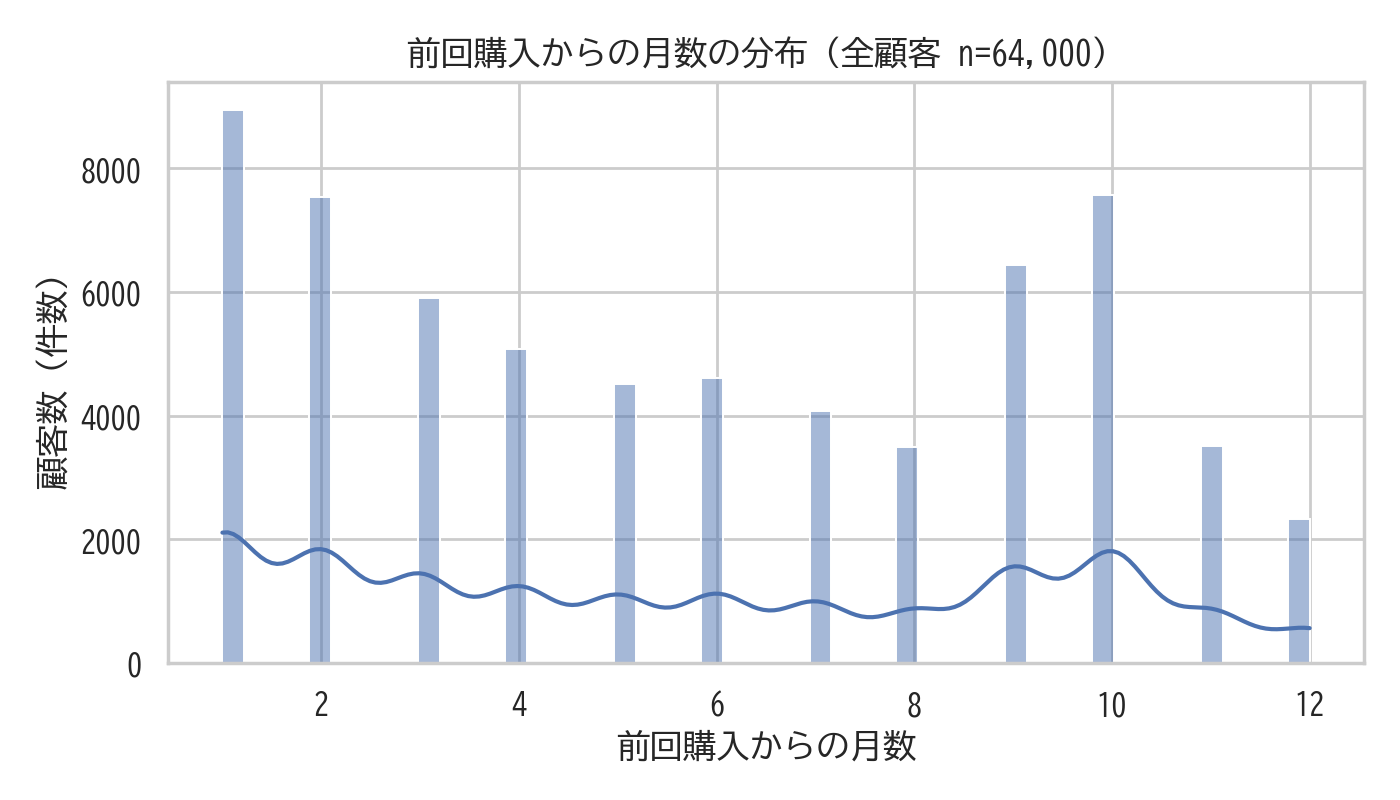
\includegraphics[width=0.88\linewidth]{../figures/dist_recency.png}
  \caption{recency（最終購入からの月数）の周辺分布}
  \label{fig:dist_recency}
\end{figure}

\begin{figure}[htbp]
  \centering
  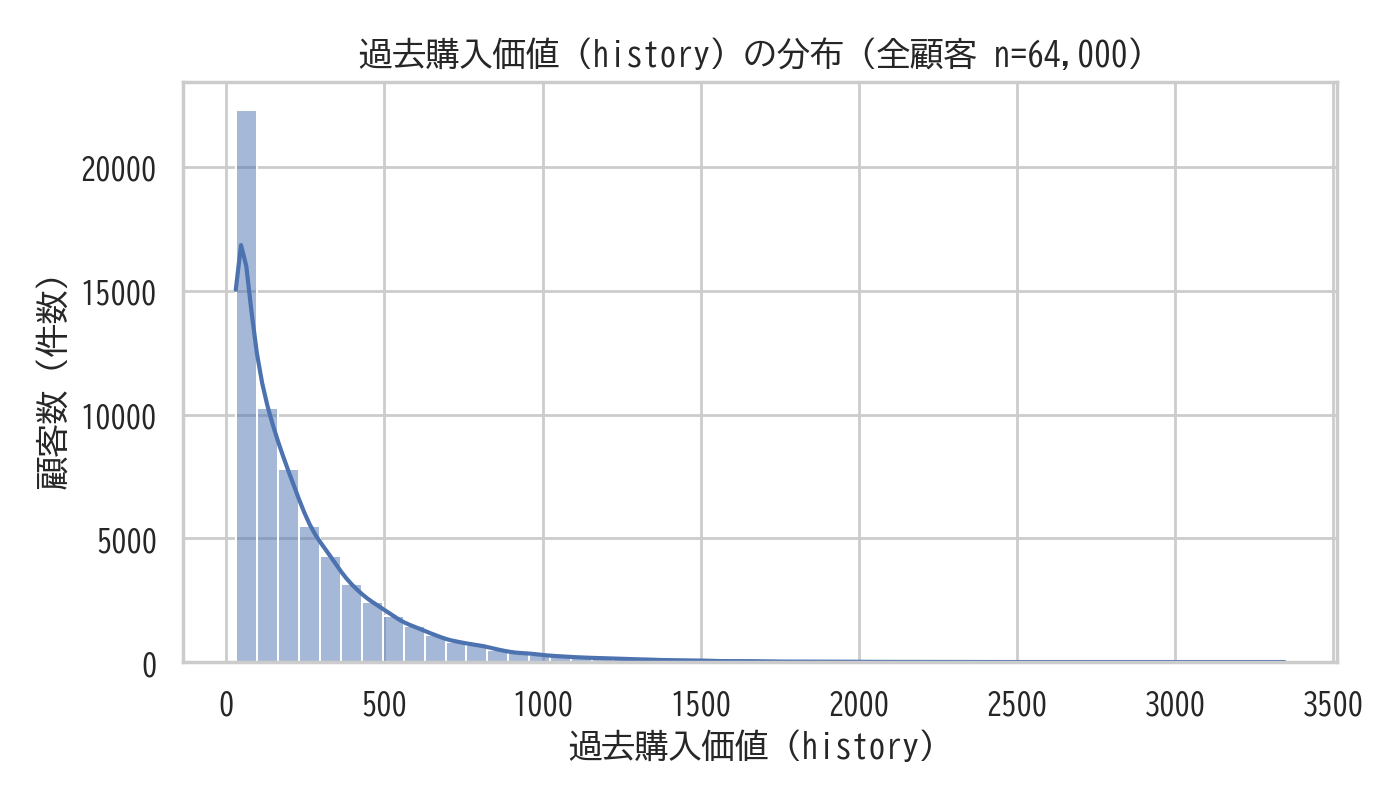
\includegraphics[width=0.88\linewidth]{../figures/dist_history.png}
  \caption{history（過去購入価値 proxy、円）の周辺分布}
  \label{fig:dist_history}
\end{figure}

\begin{figure}[htbp]
  \centering
  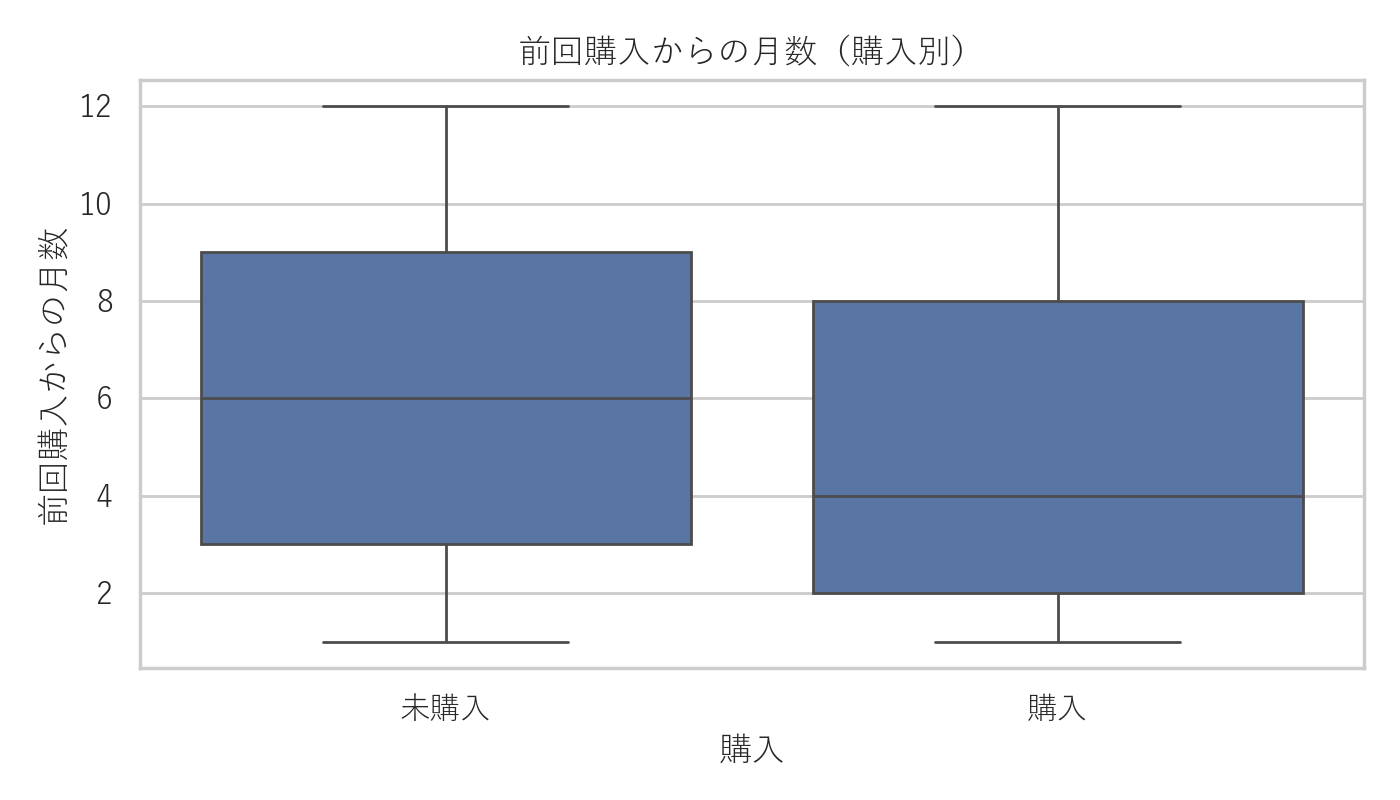
\includegraphics[width=0.88\linewidth]{../figures/box_recency_by_conversion.png}
  \caption{recency：購入有無別の箱ひげ}
  \label{fig:box_recency}
\end{figure}

\begin{figure}[htbp]
  \centering
  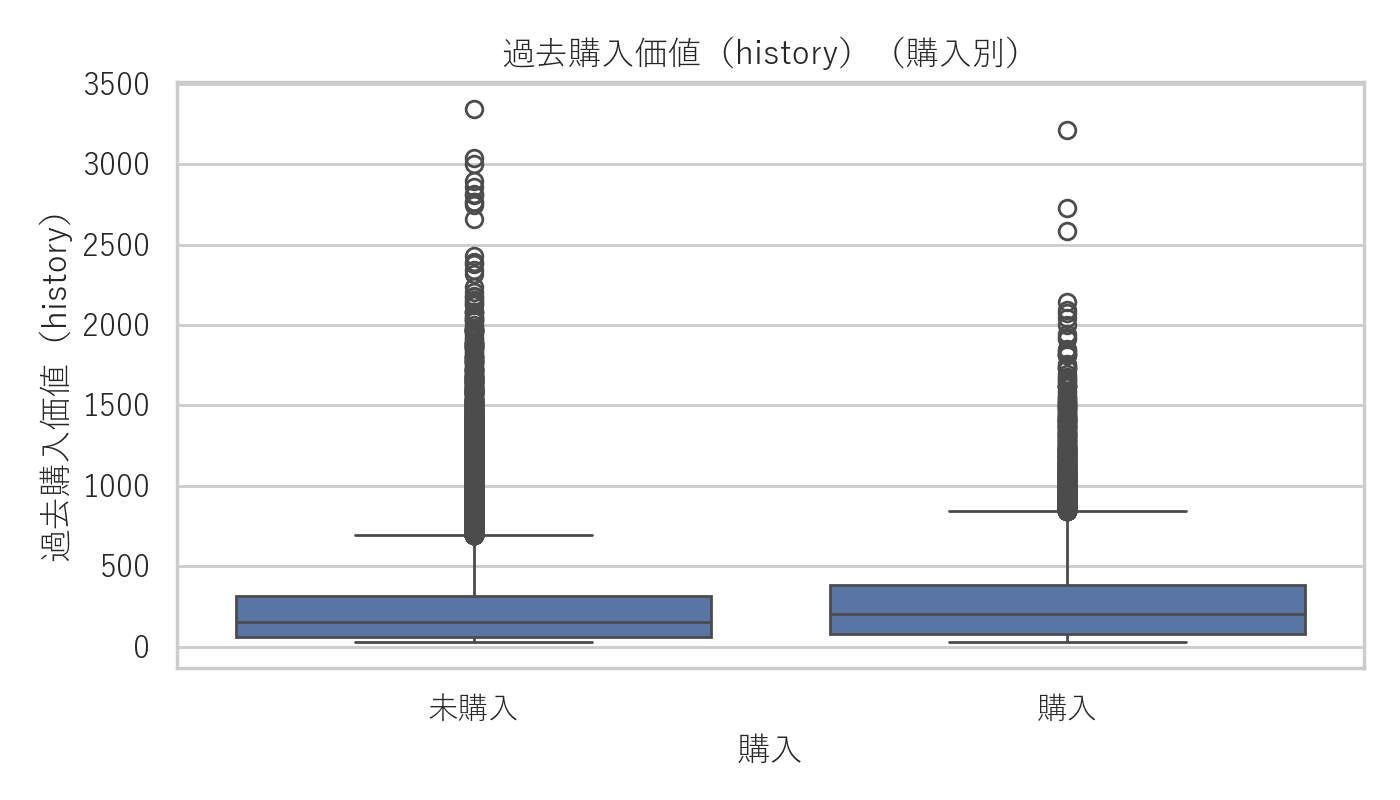
\includegraphics[width=0.88\linewidth]{../figures/box_history_by_conversion.png}
  \caption{history（円）：購入有無別の箱ひげ}
  \label{fig:box_history}
\end{figure}

\subsubsection*{解釈}
周辺分布は\textbf{接触母集団の代表性}と\textbf{外れ値・右裾}を把握するための記述統計である。
箱ひげは $\Pr(\text{共変量}\mid Y)$ の差を示すが、これは\textbf{因果効果ではない}。
特に recency と処置の割当が相関する場合（例：休眠顧客に強いオファー）、
高い条件付きCVRは\textbf{交絡}により過大評価されうる。

\subsection{オファー$\times$チャネル別の条件付きCVR}
図 \ref{fig:heat} はセルごとの標本CVRを色で表す。セル内件数が小さい組み合わせでは標準誤差が大きい。

\begin{figure}[htbp]
  \centering
  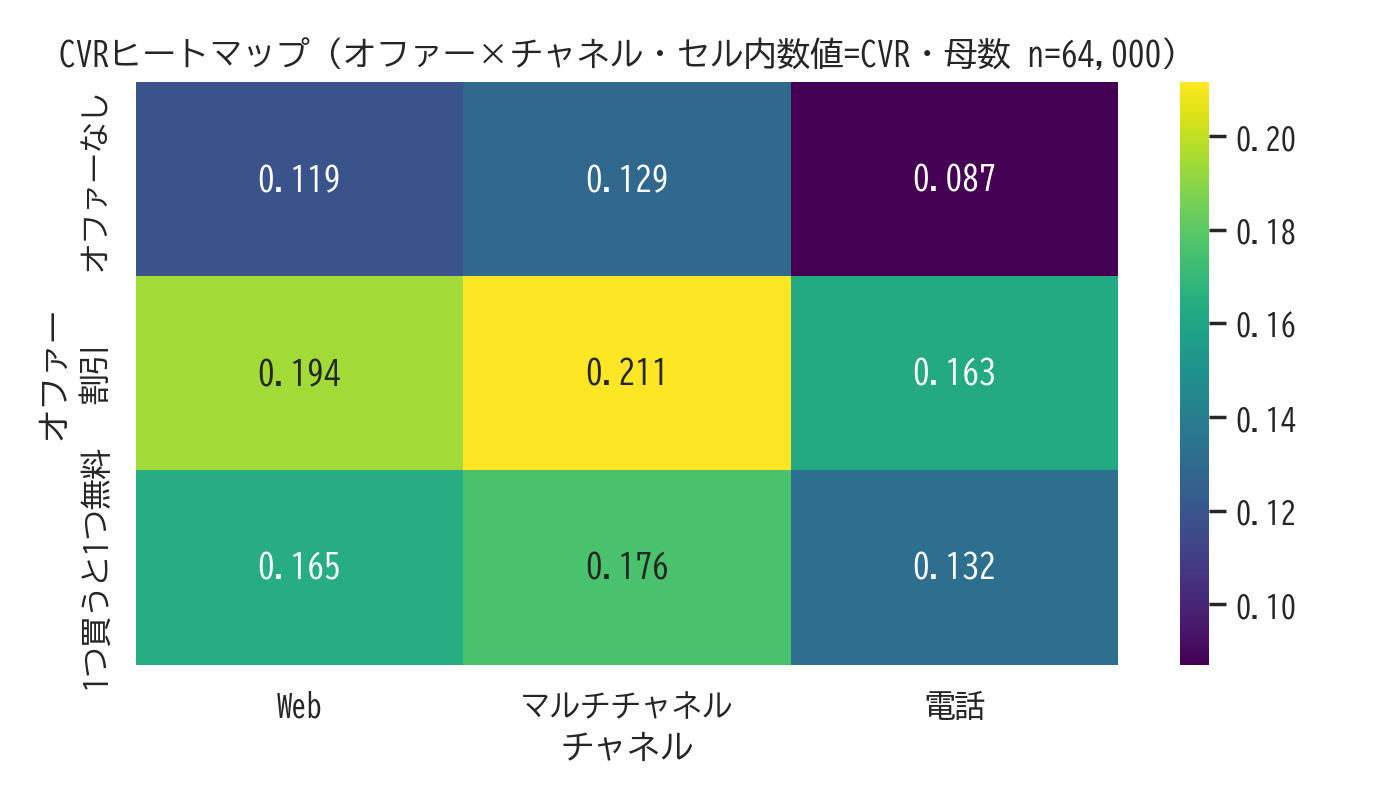
\includegraphics[width=0.92\linewidth]{../figures/heat_cvr_offer_x_channel.png}
  \caption{オファー$\times$チャネル別 CVR ヒートマップ（記述統計）}
  \label{fig:heat}
\end{figure}

\subsubsection*{解釈}
セル間のコントラストは\textbf{交互作用の存在の手がかり}となる。
ただし各セルの値は $\Pr(Y_i{=}1\mid T_i,\text{セル})$ の\textbf{観察された連関}であり、
コストを伴う期待利益の最適処置とは一致しない場合がある（後章）。

\subsection{属性別 CVR（棒グラフ）}
図 \ref{fig:cvr_offer}--\ref{fig:cvr_zip} に、オファー・チャネル・地域の\textbf{一変量層別}CVRを示す。

\begin{figure}[htbp]
  \centering
  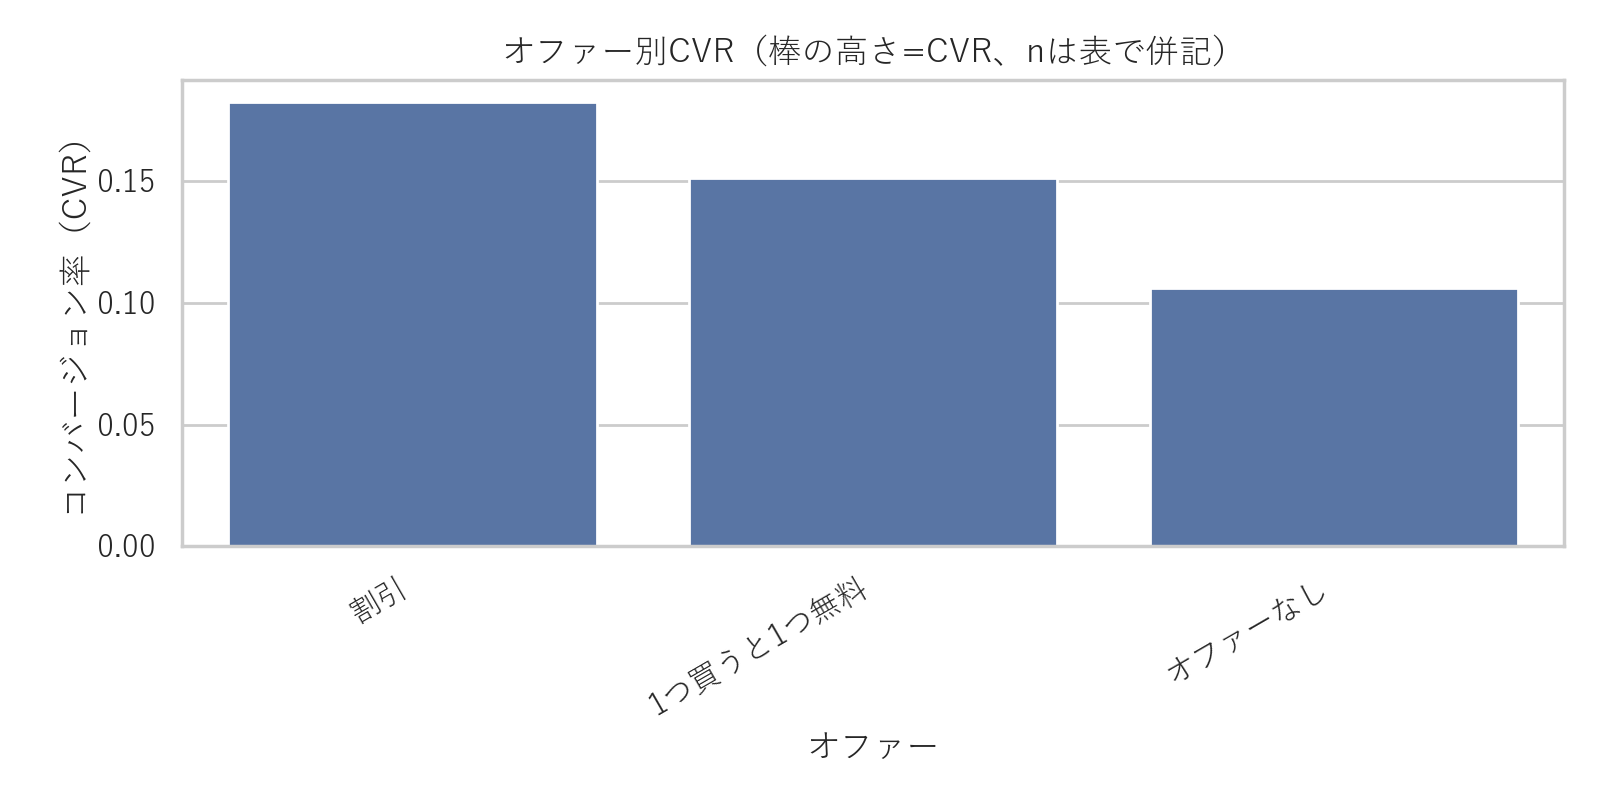
\includegraphics[width=0.72\linewidth]{../figures/cvr_by_offer.png}
  \caption{オファー別の条件付きCVR}
  \label{fig:cvr_offer}
\end{figure}

\begin{figure}[htbp]
  \centering
  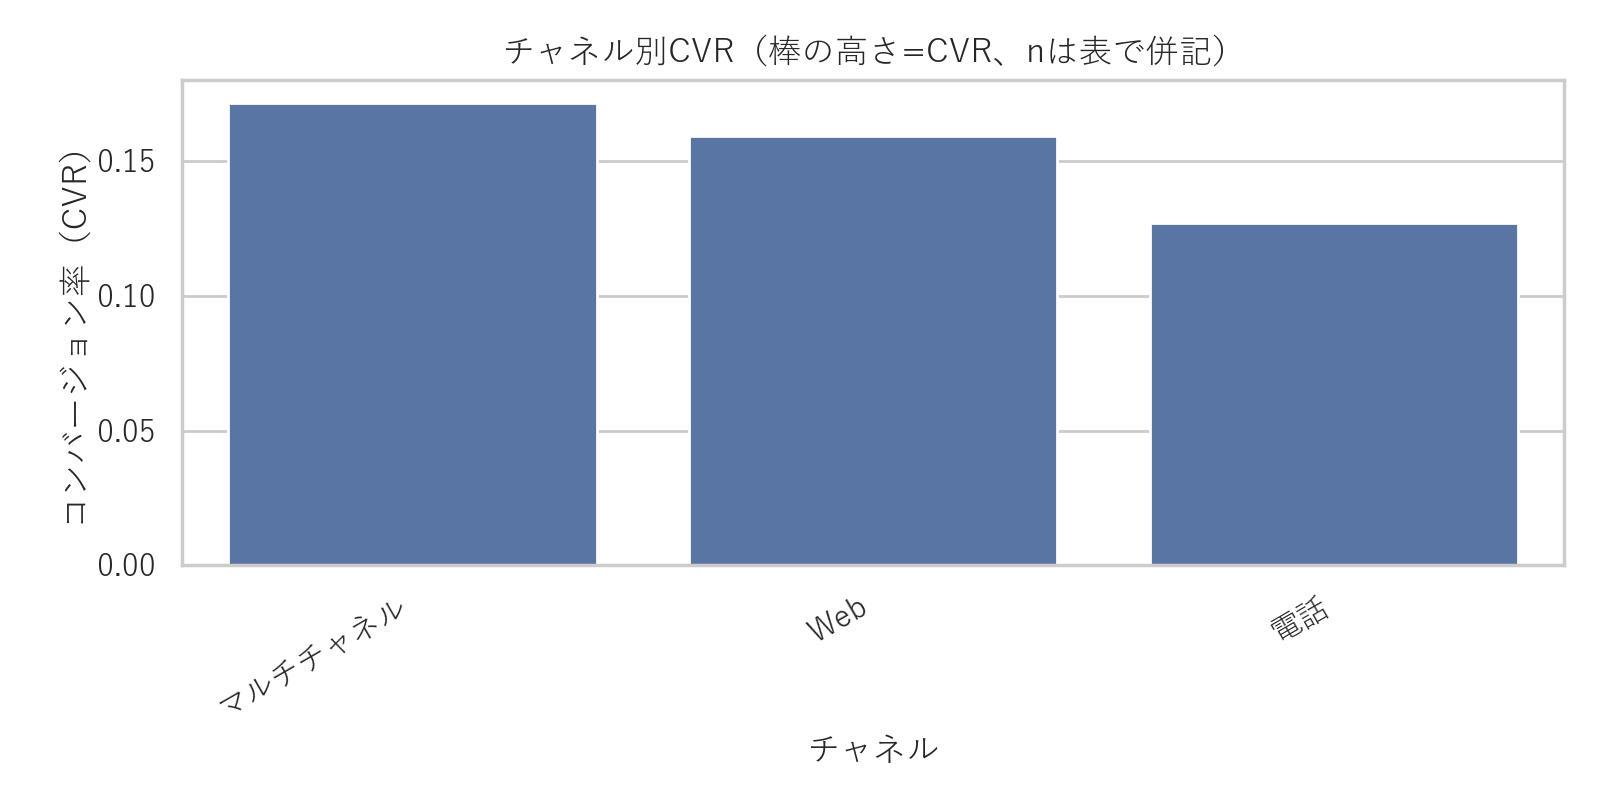
\includegraphics[width=0.72\linewidth]{../figures/cvr_by_channel.png}
  \caption{チャネル別の条件付きCVR}
  \label{fig:cvr_channel}
\end{figure}

\begin{figure}[htbp]
  \centering
  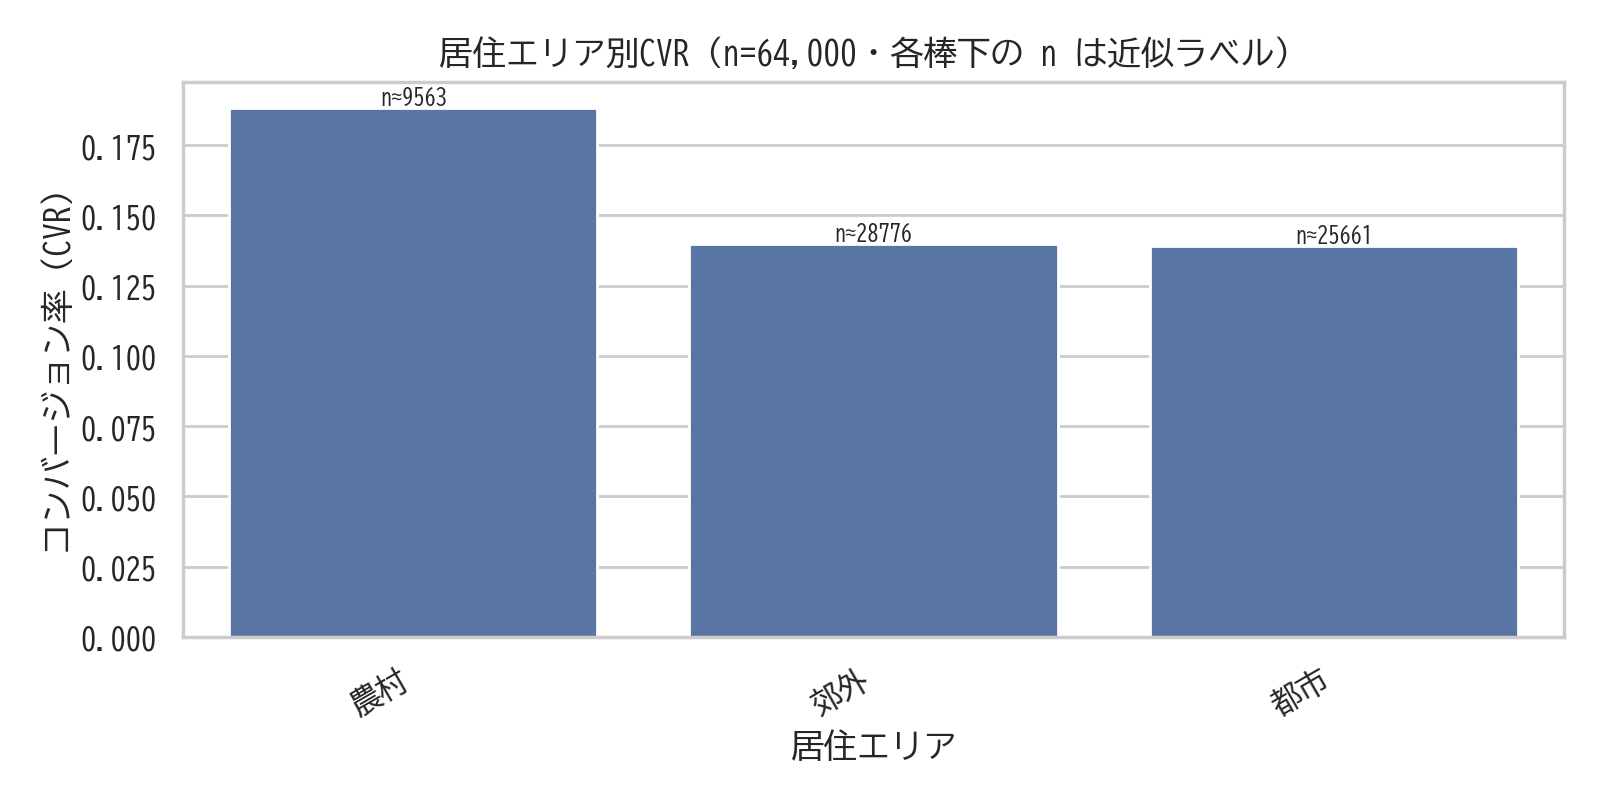
\includegraphics[width=0.72\linewidth]{../figures/cvr_by_zip_code.png}
  \caption{地域別の条件付きCVR}
  \label{fig:cvr_zip}
\end{figure}

\subsubsection*{解釈}
棒の差は\textbf{セグメント施策の動機}となるが、層の定義が処置と同時に決まる変数（過去プロモ利用など）では
\textbf{過去の処置}と\textbf{現在の割当}が絡み、因果の読み替えに注意する。
地域はセンシティブ属性の proxy になりうるため、配信ルールへの直結はガバナンスレビューを前提とする。

\section{多重検定（FDR）と効果量}

\subsection{方法}
各カテゴリ特徴量について購入との\textbf{独立性のカイ二乗検定}を行い、
Benjamini--Hochberg 手順で偽発見率（FDR）を $q$ 値として報告する。
効果量には Cramér's $V$ を併記し、$p$ 値のみに依存しない。

\begin{figure}[htbp]
  \centering
  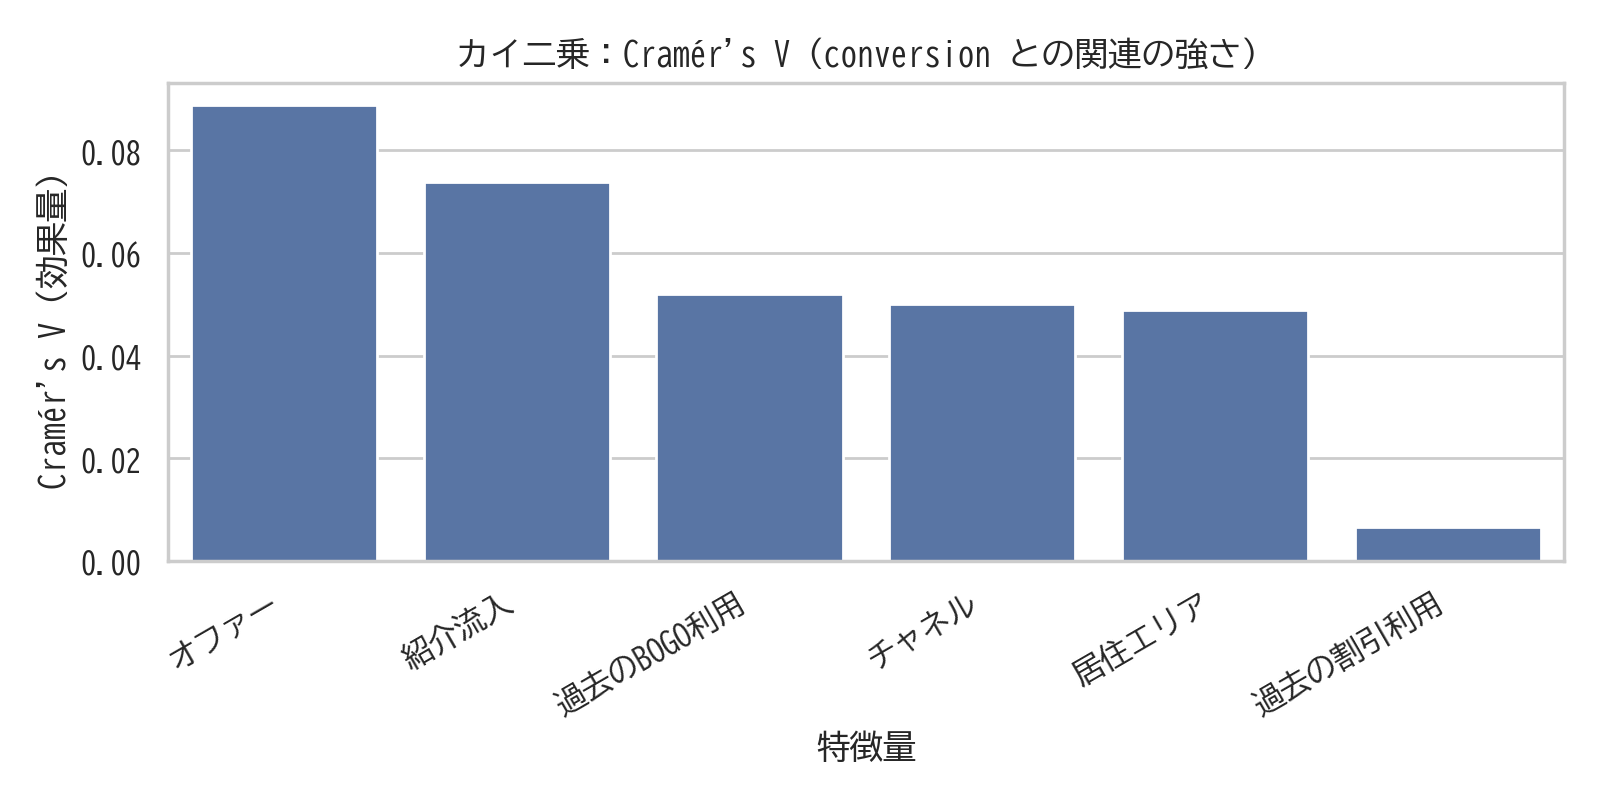
\includegraphics[width=0.75\linewidth]{../figures/improvements/chi2_cramers_v_bar.png}
  \caption{カイ二乗検定に基づく効果量（Cramér's $V$）}
  \label{fig:chi2_v}
\end{figure}

\subsubsection*{解釈}
大標本では\textbf{統計的有意 $\neq$ 実務的に大きな効果}となりやすい。
$V$ が小さい場合は、予測モデルへの寄与も限定的である可能性がある。
多数の変数が購入と関連する場合、ロジスティック回帰では\textbf{多重共線性}により係数解釈が難しくなる。

\medskip\noindent
\textbf{補足（特徴量重要度）.}
カイ二乗は\textbf{周辺}の関連スクリーニングに留まる。予測モデル内での寄与を説明するには、木系モデルに対する\textbf{SHAP}値やPermutation importanceなど、モデル条件付きの分解を併記すると「どの変数がスコアを押し上げたか」の説明が強化される（本稿の主推定はロジスティック／HGBの予測精度と政策接続が主目的）。

% 相関・OLS・LSI アブレーション節は analytics/report_tex.py が生成（final_report.md と図パス整合）
\section{相関と補助的重回帰（history）}

\subsection{Pearson 相関（数値・二値）}
図 \ref{fig:corr} は主要な数値・二値列の Pearson 相関を\textbf{下三角のみ}表示したものである（重複セルを避ける）。
強い相関は特徴設計上の\textbf{冗長性}の手がかりとなるが、因果ではない。

\begin{figure}[htbp]
  \centering
  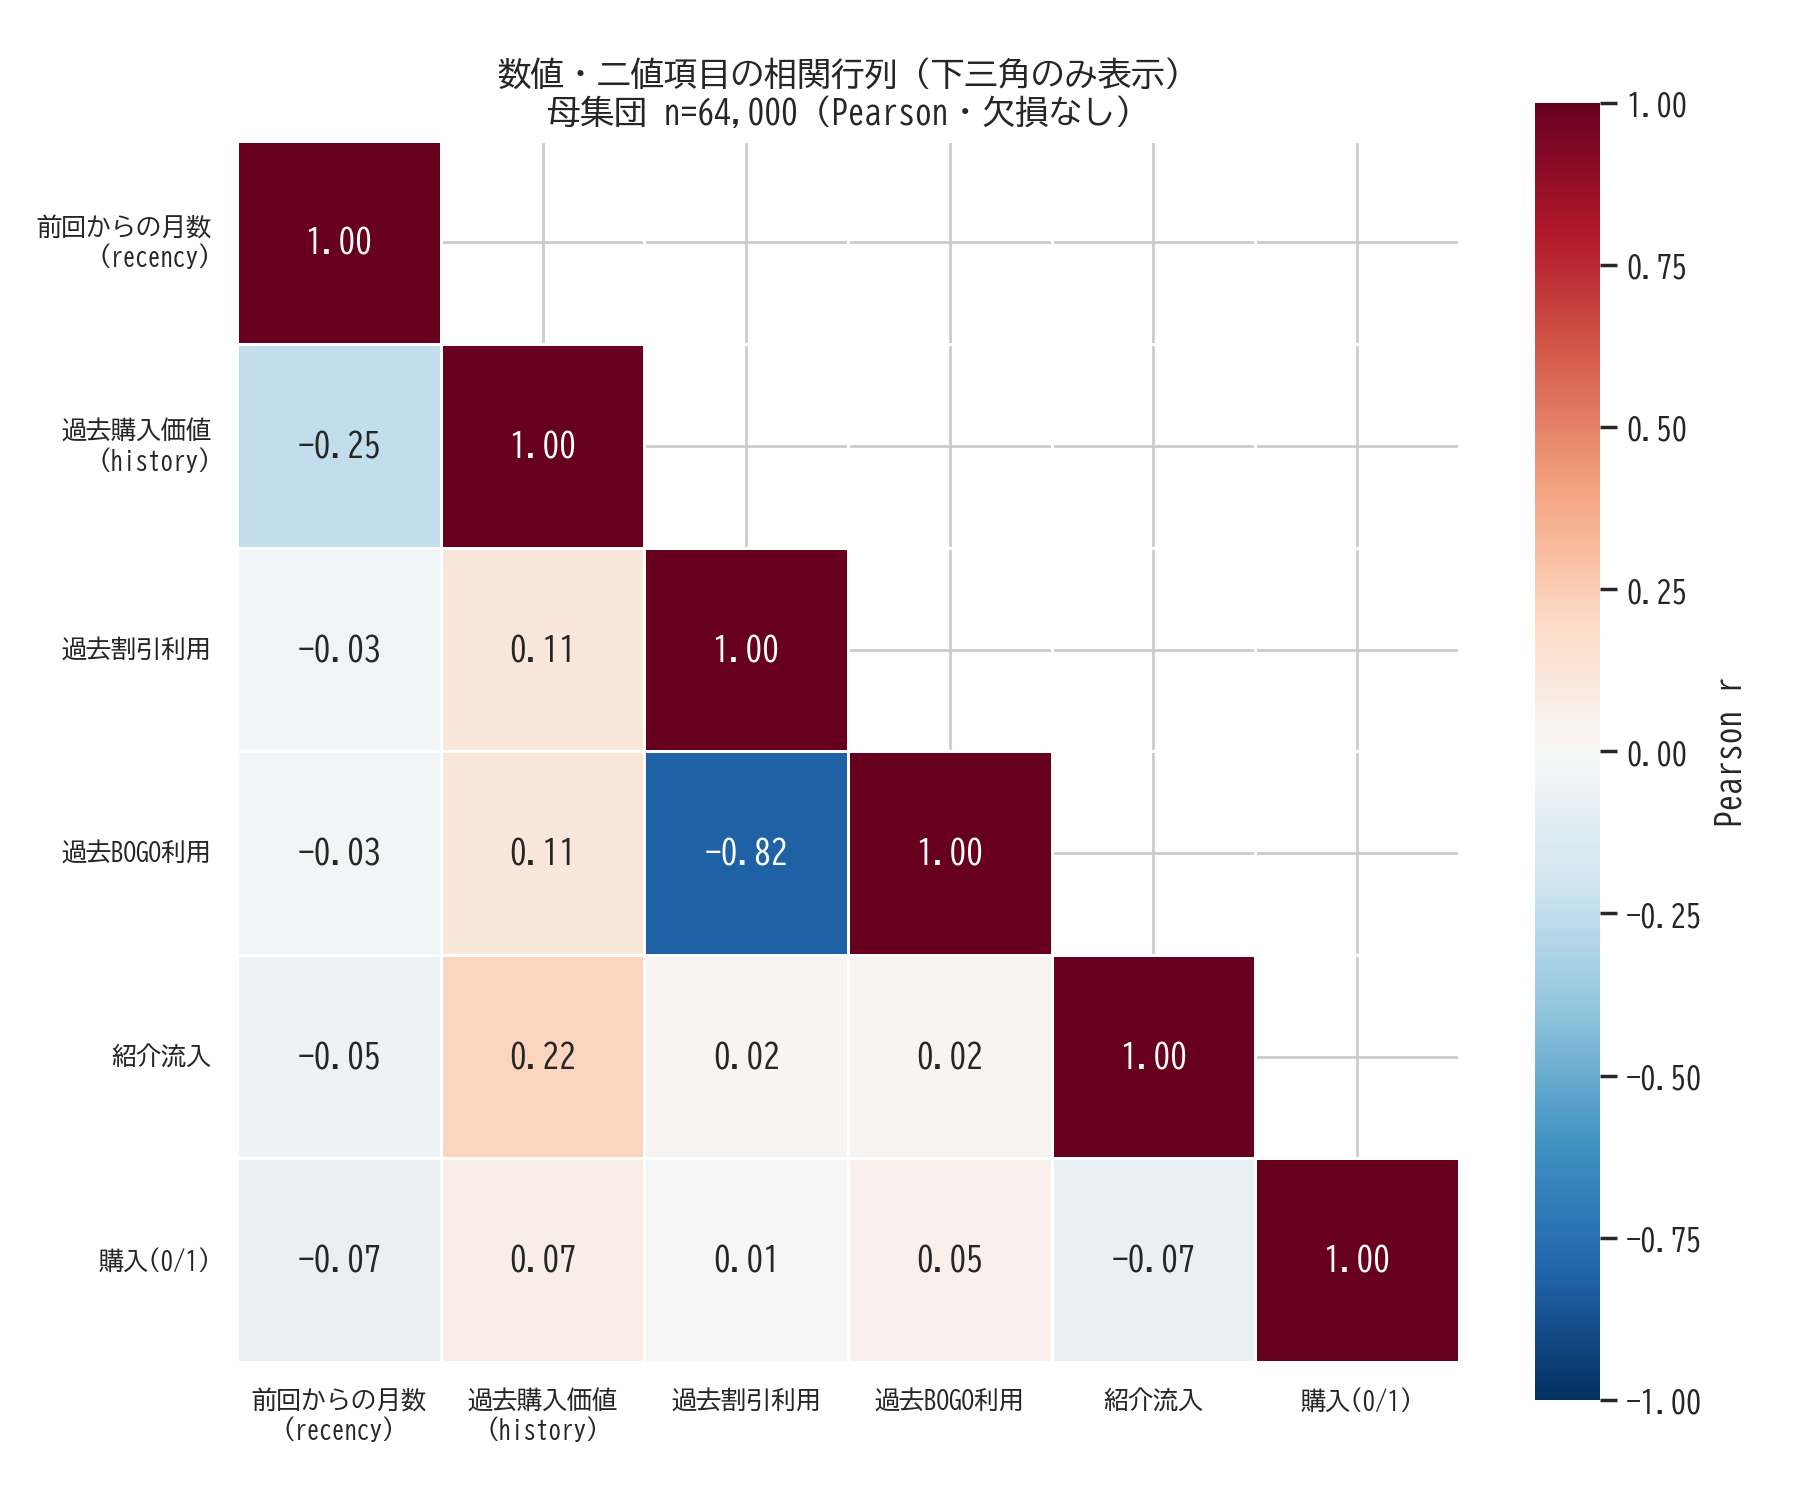
\includegraphics[width=0.92\linewidth]{../figures/improvements/corr_numeric_detailed.png}
  \caption{相関行列（Pearson、下三角）}
  \label{fig:corr}
\end{figure}

\begin{figure}[htbp]
  \centering
  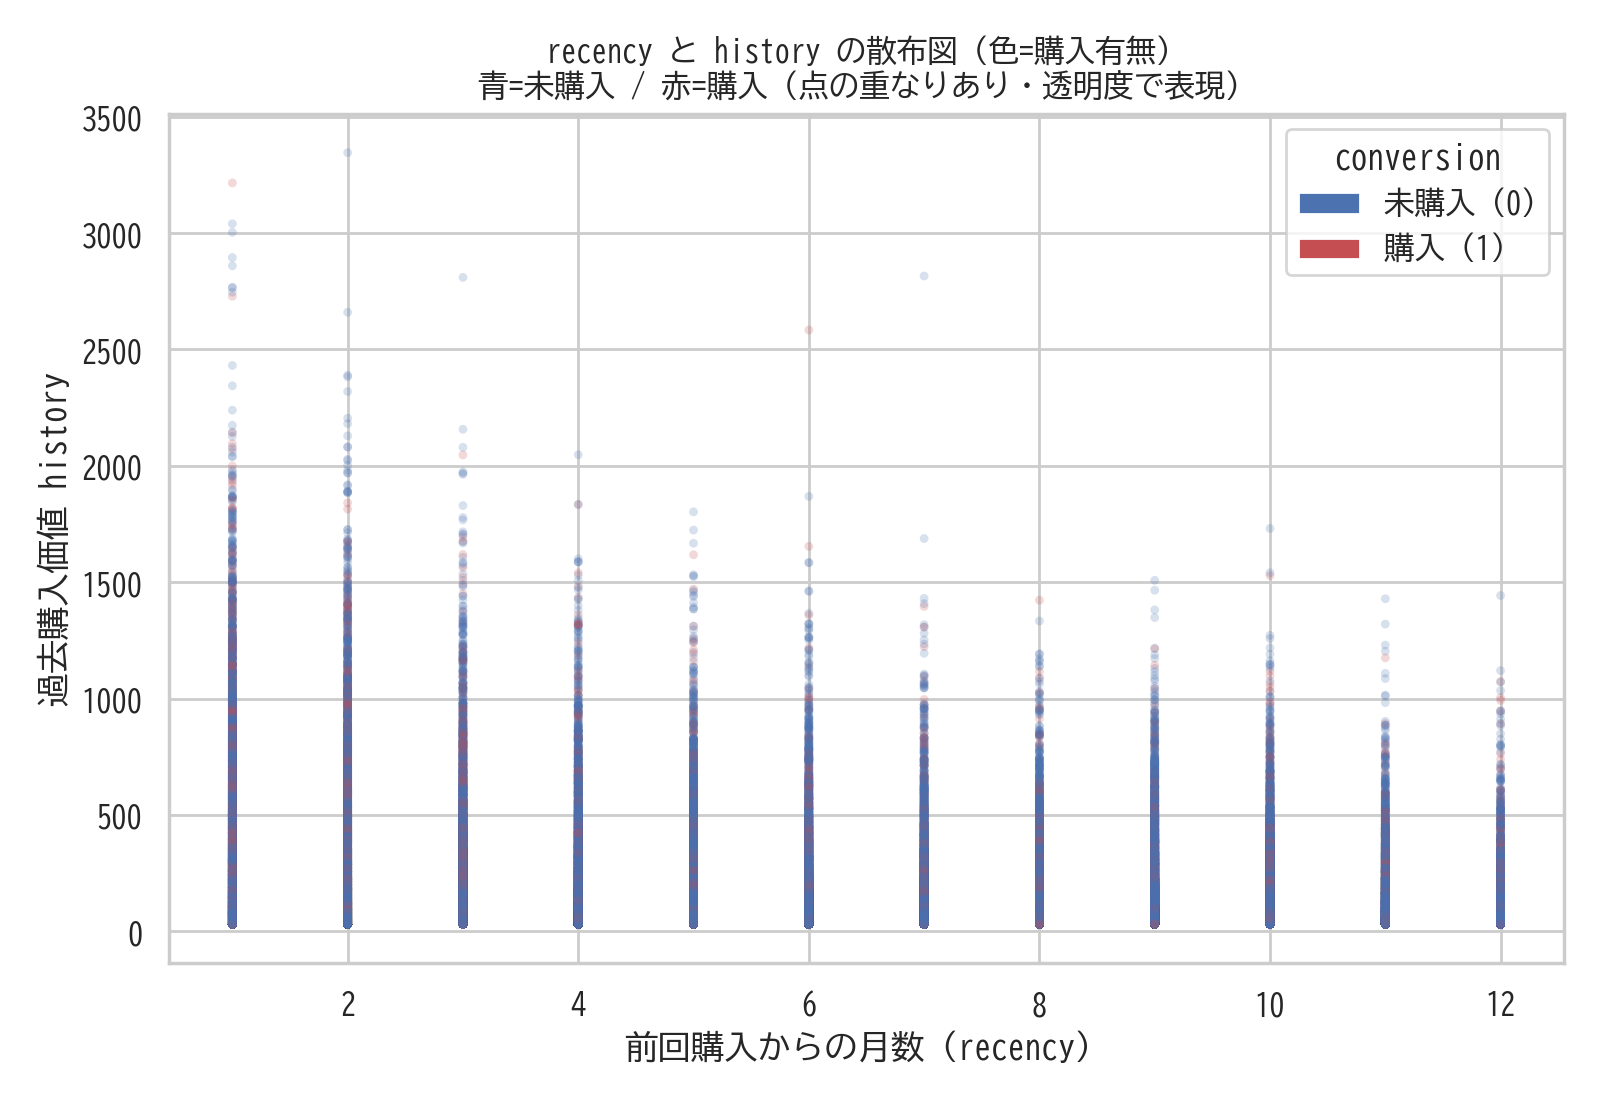
\includegraphics[width=0.88\linewidth]{../figures/improvements/scatter_recency_history_by_conversion.png}
  \caption{recency と history の散布図（色は購入有無）}
  \label{fig:scatter_rh}
\end{figure}

\subsection{OLS（目的変数を history）}
演習で例示される重回帰に対応するため、連続の \texttt{history} を目的変数とした OLS（説明変数は \texttt{recency}, \texttt{used\_discount}, \texttt{used\_bogo}, \texttt{is\_referral}、ロバスト分散 HC1）を付す。
購入予測そのものは次節以降のロジスティック回帰が主である。係数表は \texttt{artifacts/ols\_history\_coefficients.csv}。

\begin{figure}[htbp]
  \centering
  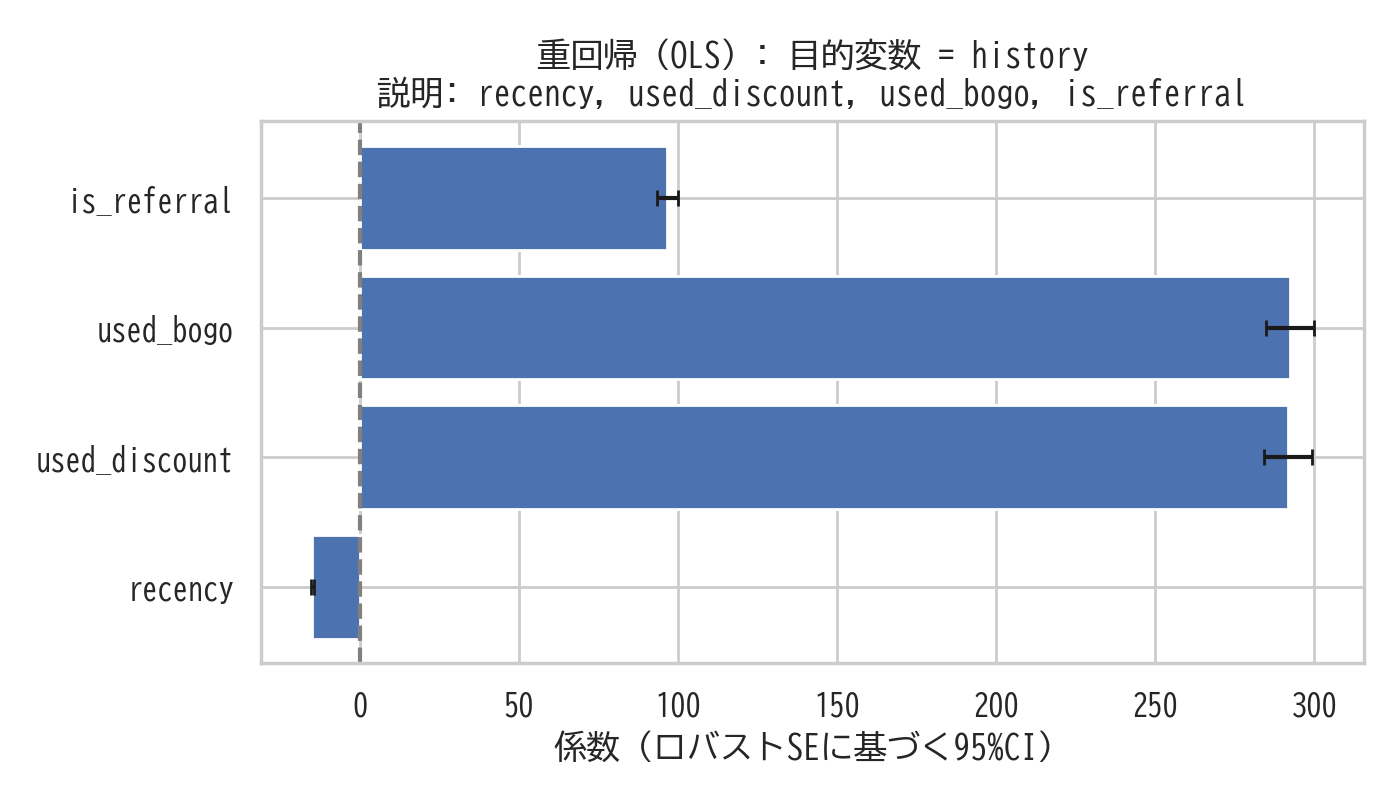
\includegraphics[width=0.78\linewidth]{../figures/improvements/ols_history_coefficients.png}
  \caption{OLS 係数と 95\% 信頼区間（history を目的変数）}
  \label{fig:ols_hist}
\end{figure}

\section{LSI類似表現と分類アブレーション}

各行を英語テンプレの短文に変換し、\textbf{訓練標本のみ}に fit した TF-IDF と TruncatedSVD（次元は \texttt{artifacts/lsi\_tfidf\_diag.json}）を特徴に連結し、
ロジスティック回帰のホールドアウト性能を \textbf{BASE のみ} と比較する（外部 API 不要）。
図 \ref{fig:lsi_ab} は同一分割における AUC / Brier / AP / TopK\% CVR の対比である。

\begin{figure}[htbp]
  \centering
  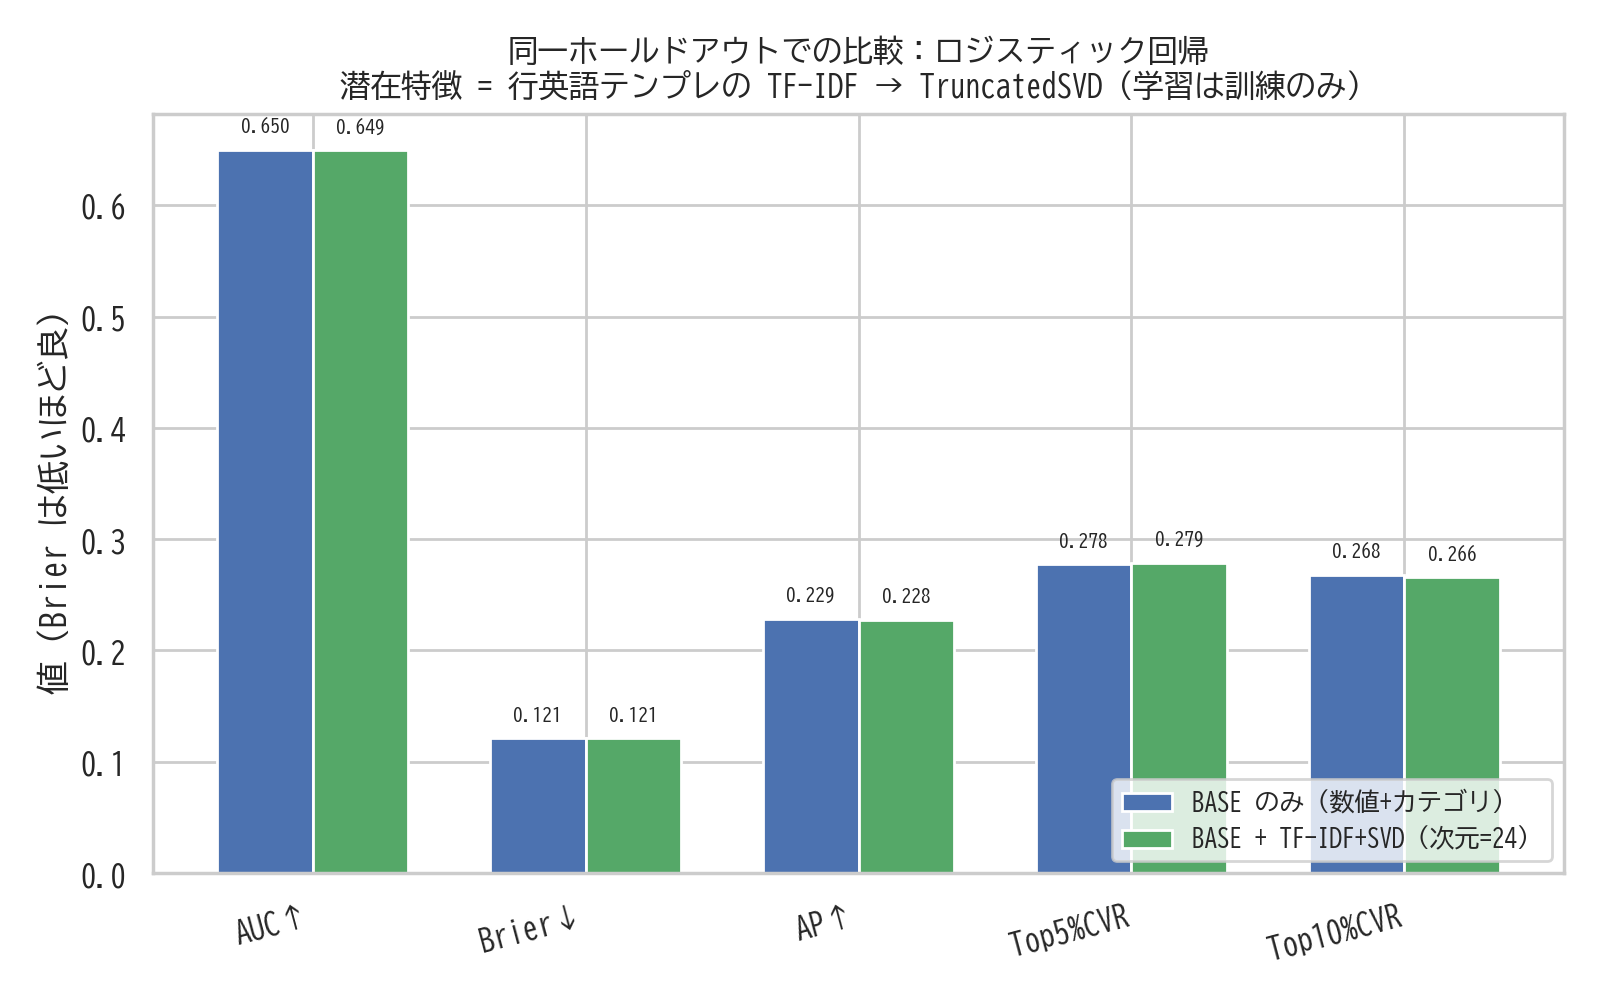
\includegraphics[width=0.92\linewidth]{../figures/improvements/ablation_base_vs_lsi_logreg.png}
  \caption{BASE vs BASE+TF-IDF+SVD（同一ホールドアウト・値ラベル付き棒）}
  \label{fig:lsi_ab}
\end{figure}


\section{予測モデル（ROC・校正・PR）}
\label{sec:pred}

\noindent\textbf{（この節のねらい）}
顧客ごとに\textbf{購入しやすさ}をスコア化し、\textbf{限られた接触枠}で誰を優先するかの材料にする。
AUC/PRは\textbf{順位付けの良さ}、校正は\textbf{確率の絶対値の信頼性}（期待利益計算に効く）を見る。

\subsection{評価指標の意味}
\textbf{AUC（ROC）}: 閾値を掃引したときの誤警報率と検出力のトレードオフを要約したランキング指標。
\textbf{Brier スコア}: 確率予測の二乗誤差。
\textbf{校正曲線}: 予測確率ビンにおける観測頻度との一致（較正）。
\textbf{PR 曲線・AP}: 陽性クラスが稀なときの precision--recall トレードオフとその要約。

\begin{figure}[htbp]
  \centering
  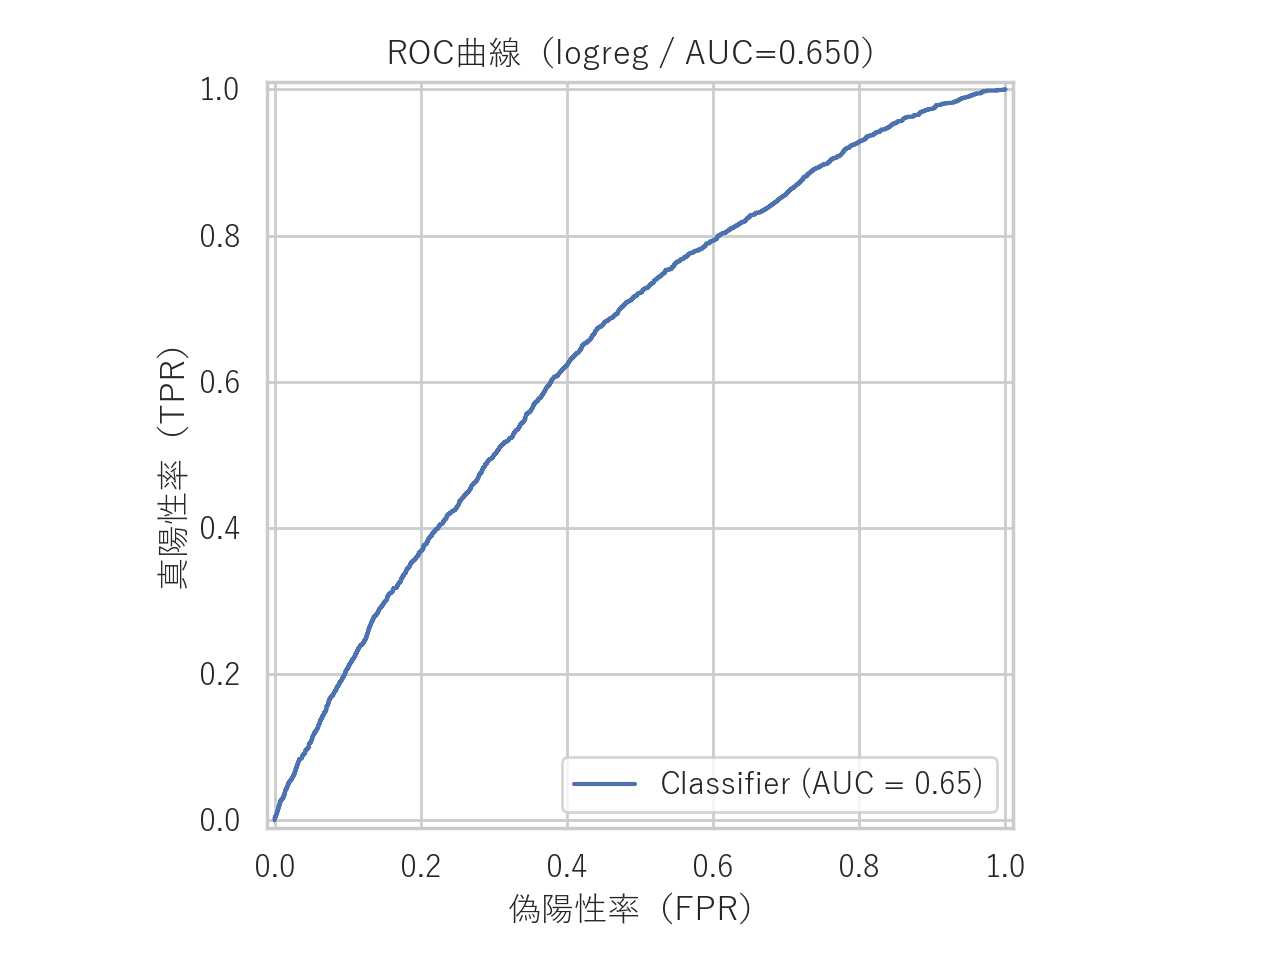
\includegraphics[width=0.72\linewidth]{../figures/roc_logreg.png}
  \caption{ROC 曲線（logistic regression、ホールドアウト）}
  \label{fig:roc_logreg}
\end{figure}

\begin{figure}[htbp]
  \centering
  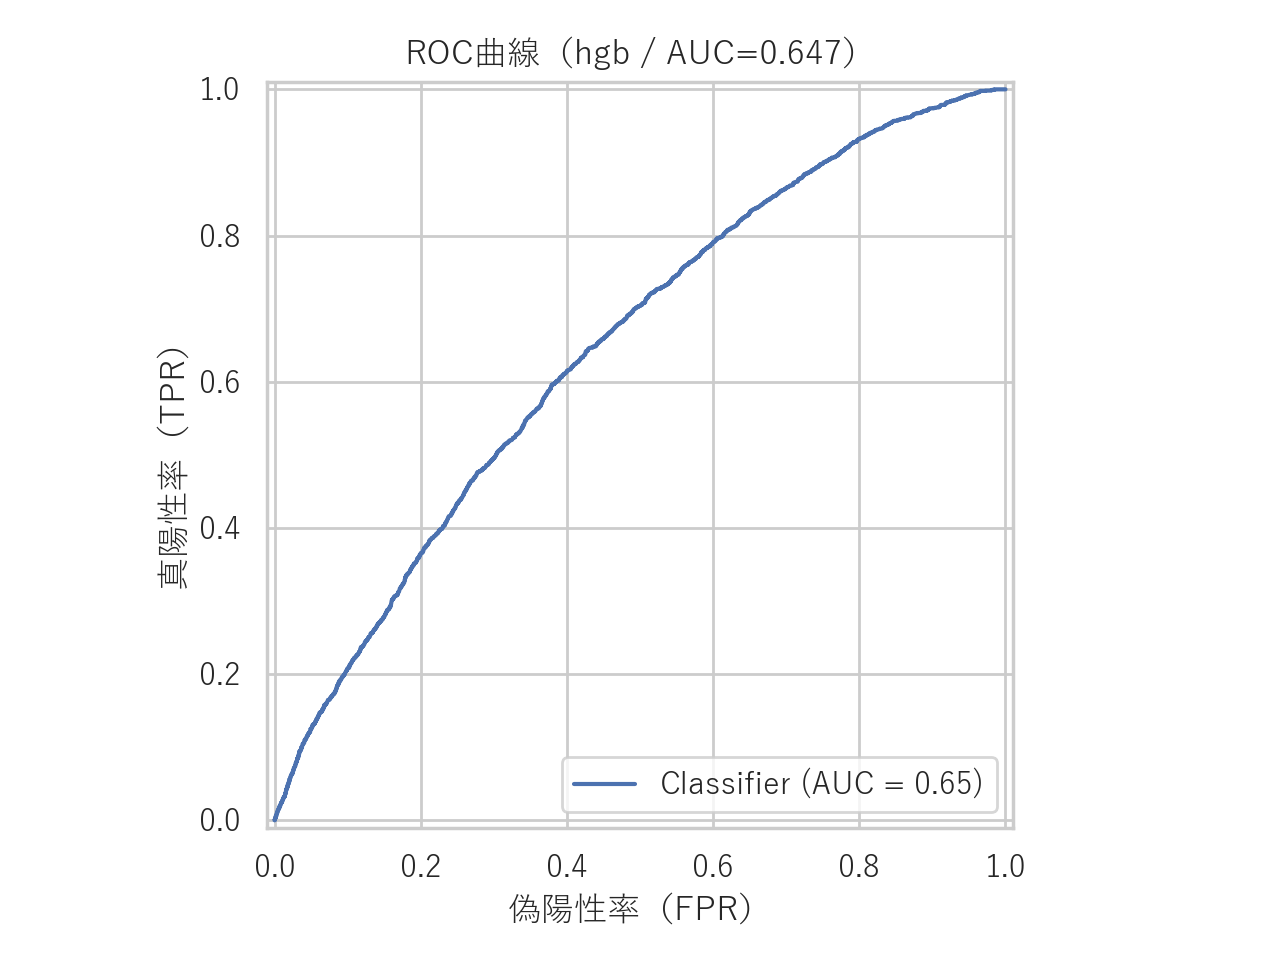
\includegraphics[width=0.72\linewidth]{../figures/roc_hgb.png}
  \caption{ROC 曲線（histogram-based gradient boosting、ホールドアウト）}
  \label{fig:roc_hgb}
\end{figure}

\begin{figure}[htbp]
  \centering
  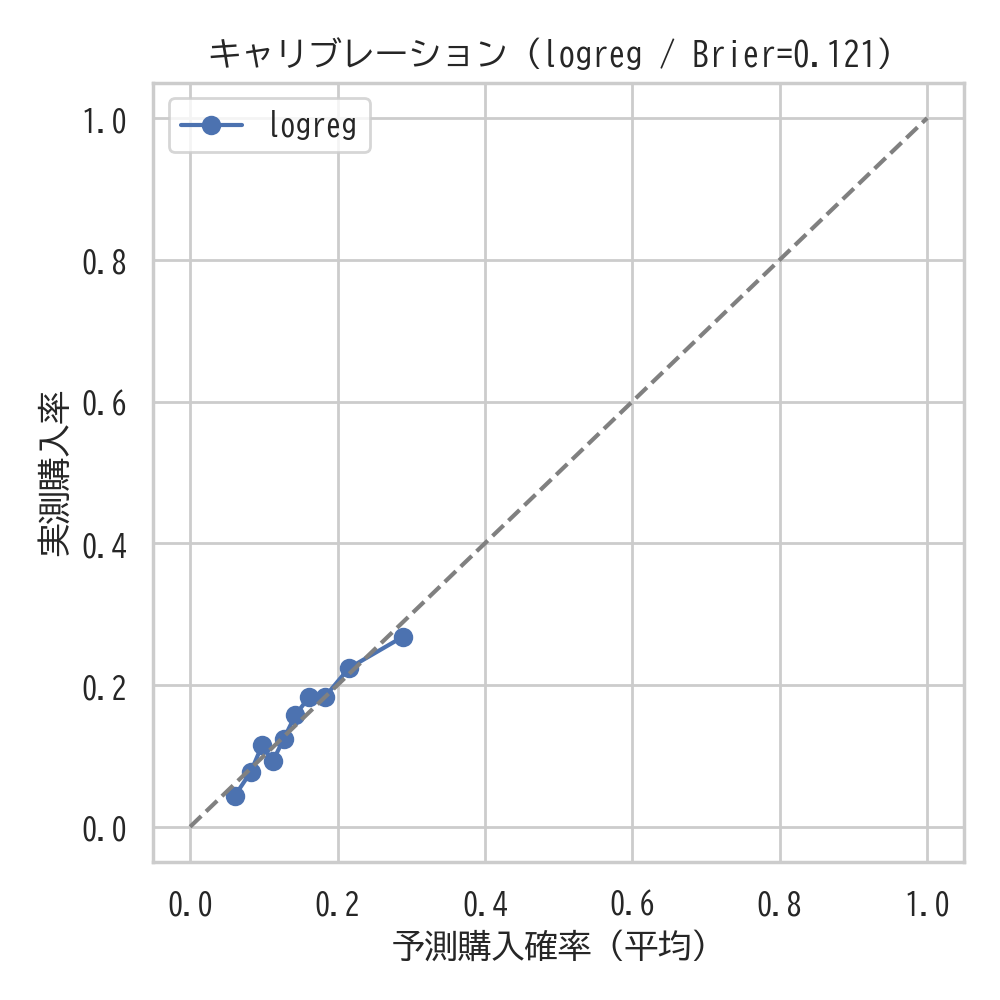
\includegraphics[width=0.72\linewidth]{../figures/calibration_logreg.png}
  \caption{校正曲線（logistic regression）}
  \label{fig:cal_logreg}
\end{figure}

\begin{figure}[htbp]
  \centering
  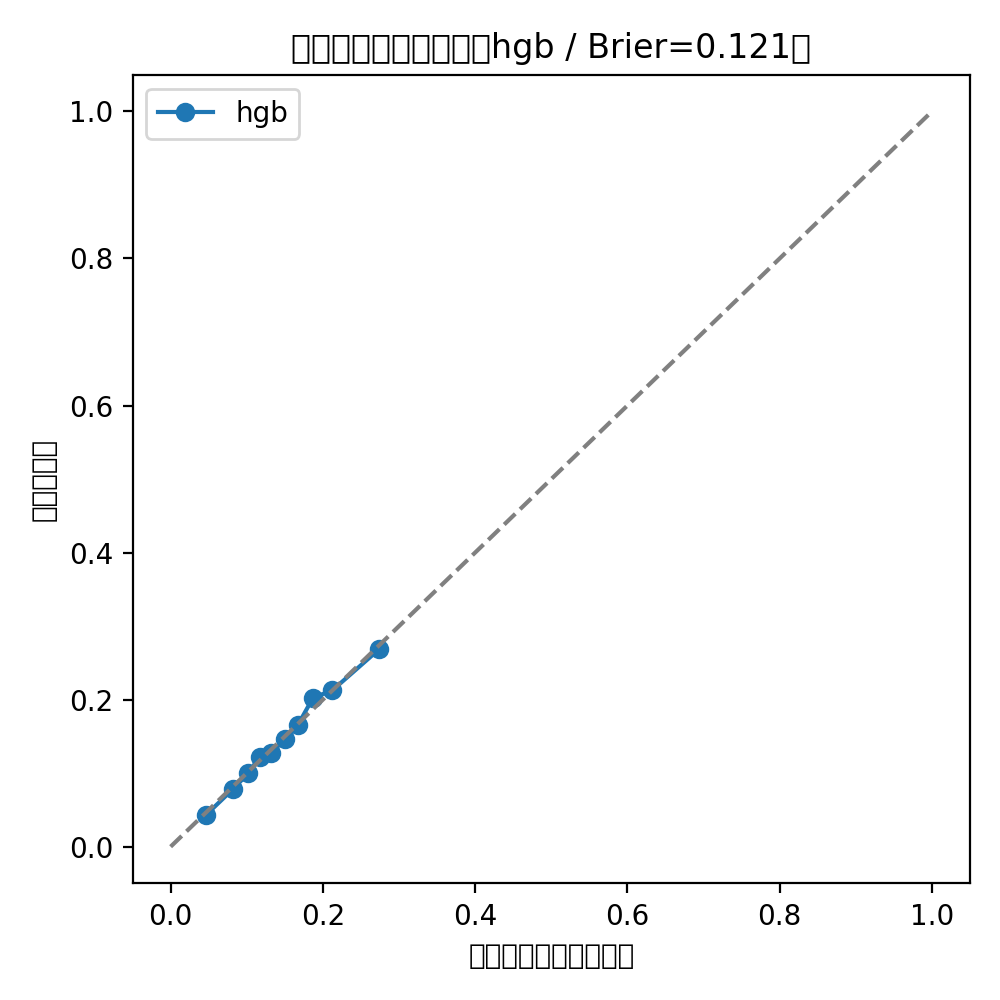
\includegraphics[width=0.72\linewidth]{../figures/calibration_hgb.png}
  \caption{校正曲線（HGB）}
  \label{fig:cal_hgb}
\end{figure}

\subsubsection*{解釈}
AUC が中程度のとき、完全分離は達成されておらず、\textbf{ターゲティングの上限}が統計的に制限される。
期待利益は確率の\textbf{絶対水準}に依存するため、校正の崩れは\textbf{政策の順位入れ替え}を招きうる。
運用では ECE やドリフト監視が有効である。
\textbf{閾値例（運用ゲートのたたき台）:} 10ビンECEが\textbf{訓練時比 +0.05}を超えたら再較正を検討、\textbf{+0.08}超なら配信縮小（ホールドアウト比較と併用）。
Brier悪化がベースライン比\textbf{10\,\%相対}超過ならモデル差し替え候補とする（組織で合意したうえで固定化する）。

\begin{figure}[htbp]
  \centering
  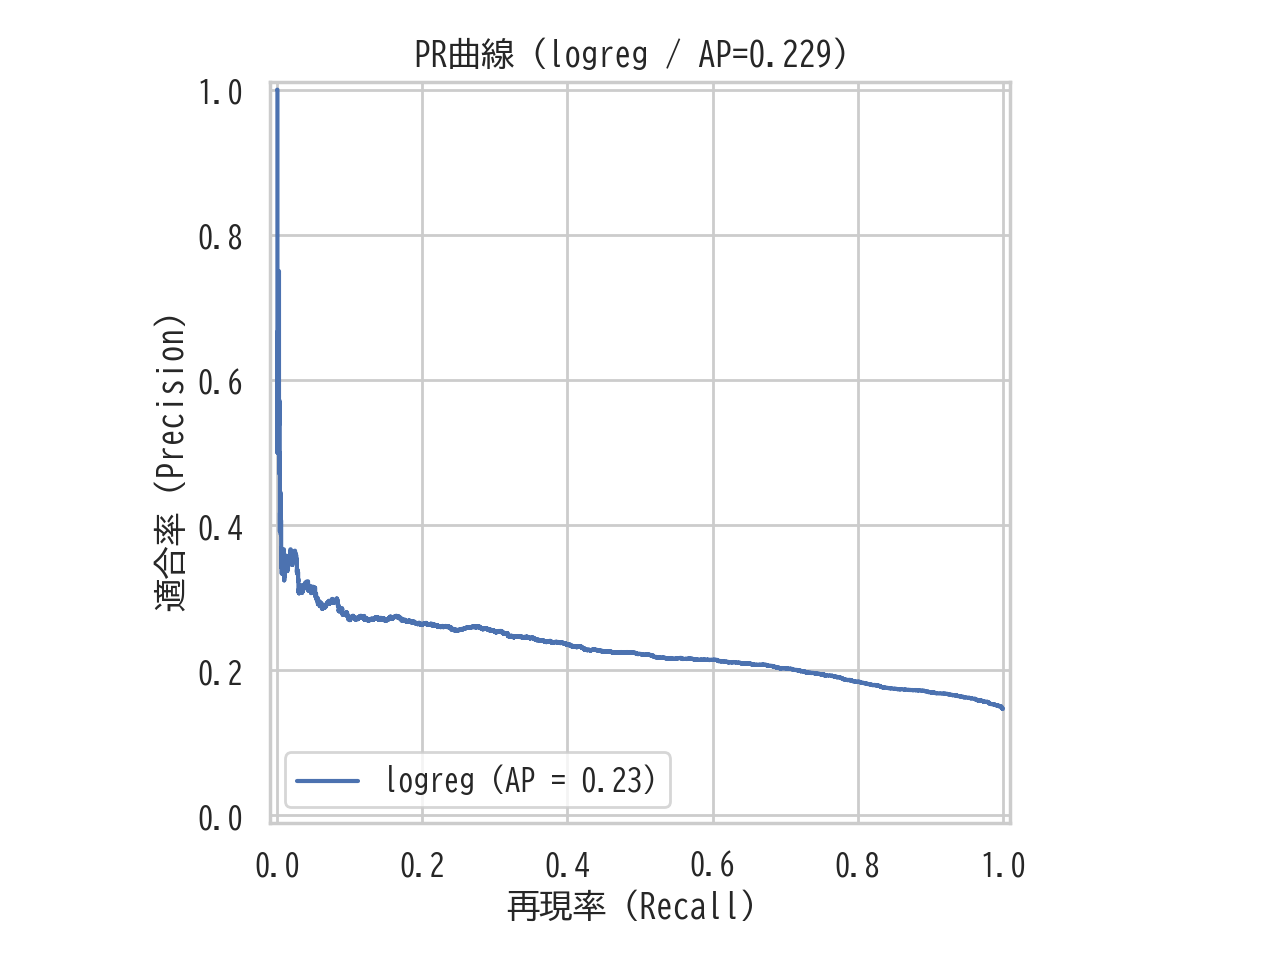
\includegraphics[width=0.72\linewidth]{../figures/improvements/pr_curve_logreg.png}
  \caption{Precision--Recall 曲線（logistic regression）}
  \label{fig:pr_logreg}
\end{figure}

\begin{figure}[htbp]
  \centering
  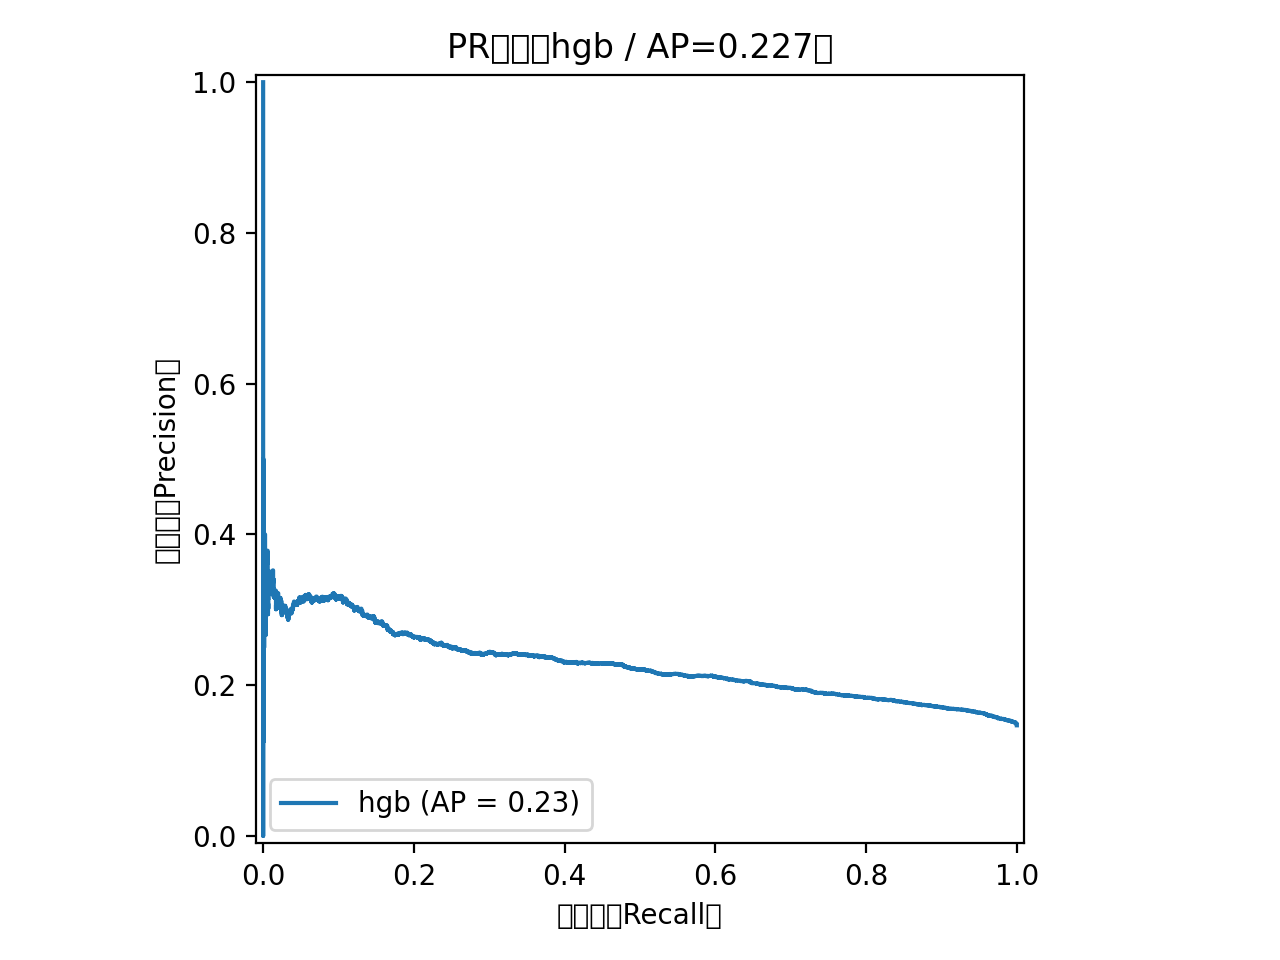
\includegraphics[width=0.72\linewidth]{../figures/improvements/pr_curve_hgb.png}
  \caption{Precision--Recall 曲線（HGB）}
  \label{fig:pr_hgb}
\end{figure}

\subsubsection*{解釈}
AP と TopK\% CVR（表）は\textbf{限られた接触枠}のもとでの運用品質に直結する。
木系が線形より Top 尾で有利な場合があり、ROC の差以上に政策評価に効くことがある。

\section{因果推論（傾向スコア、DR、ブートストラップ）}
\label{sec:causal}

\noindent\textbf{（この節のねらい）}
観察されたオファー・チャネル割当のもとで、処置ごとの購入率の\textbf{参考比較}をする。
傾向スコアと結果モデルを組み合わせたDRは\textbf{どちらか一方が少し誤っていても頑健}という性質があるが、\textbf{未観測の交絡}があると根本的には残る。

\subsection{DR 推定量（参考）}
二重頑健推定の考え方は \cite{BangRobins2005}、方策評価への応用は \cite{Dudik2011} などを参照。
処置 $t \in \mathcal{T}$ について、本実装で用いる DR 形式は次の標本平均である：
\begin{equation}
  \label{eq:dr}
  \muDRhat(t)
  = \frac{1}{n} \sum_{i=1}^{n}
  \left\{
    \pihat(t, X_i)
    + \frac{\ind\{T_i = t\}}{\hehat(t \mid X_i)}
    \,\bigl( Y_i - \pihat(t, X_i) \bigr)
  \right\}.
\end{equation}
ここで $\hehat$ は多値ロジスティック傾向、$\pihat$ は処置を特徴量に含む結果モデル（ロジスティック）から得る。
\textbf{クリップ}を $\hehat$ に施し、極端な IPW 重みを抑制する（\texttt{PROPENSITY\_CLIP}）。

\subsection{実装上の注意（同一データ学習）}
本パイプラインでは、傾向・結果モデルを\textbf{同一学習標本}上でフィットし、\textbf{同一標本}で式 \eqref{eq:dr} を評価している。
一般にこれは\textbf{ナイーブで楽観的}となりうる。厳密にはサンプル分割や\textbf{cross-fitting} により
「自分で学習したデータで評価しない」手続きが推奨される。
\textbf{本稿で cross-fitting を最終報告に組み込まない理由}は、(i)~演習レポートの実装コストと可読性、(ii)~既存パイプラインがホールドアウト再学習・OOF政策評価で\textbf{同種の過信}を別経路から監視している、のトレードオフによる（拡張は今後の方針）。
本稿では\textbf{ホールドアウト再学習}による棒グラフ比較で、その\textbf{ギャップの大きさ}を監視する。

\begin{figure}[htbp]
  \centering
  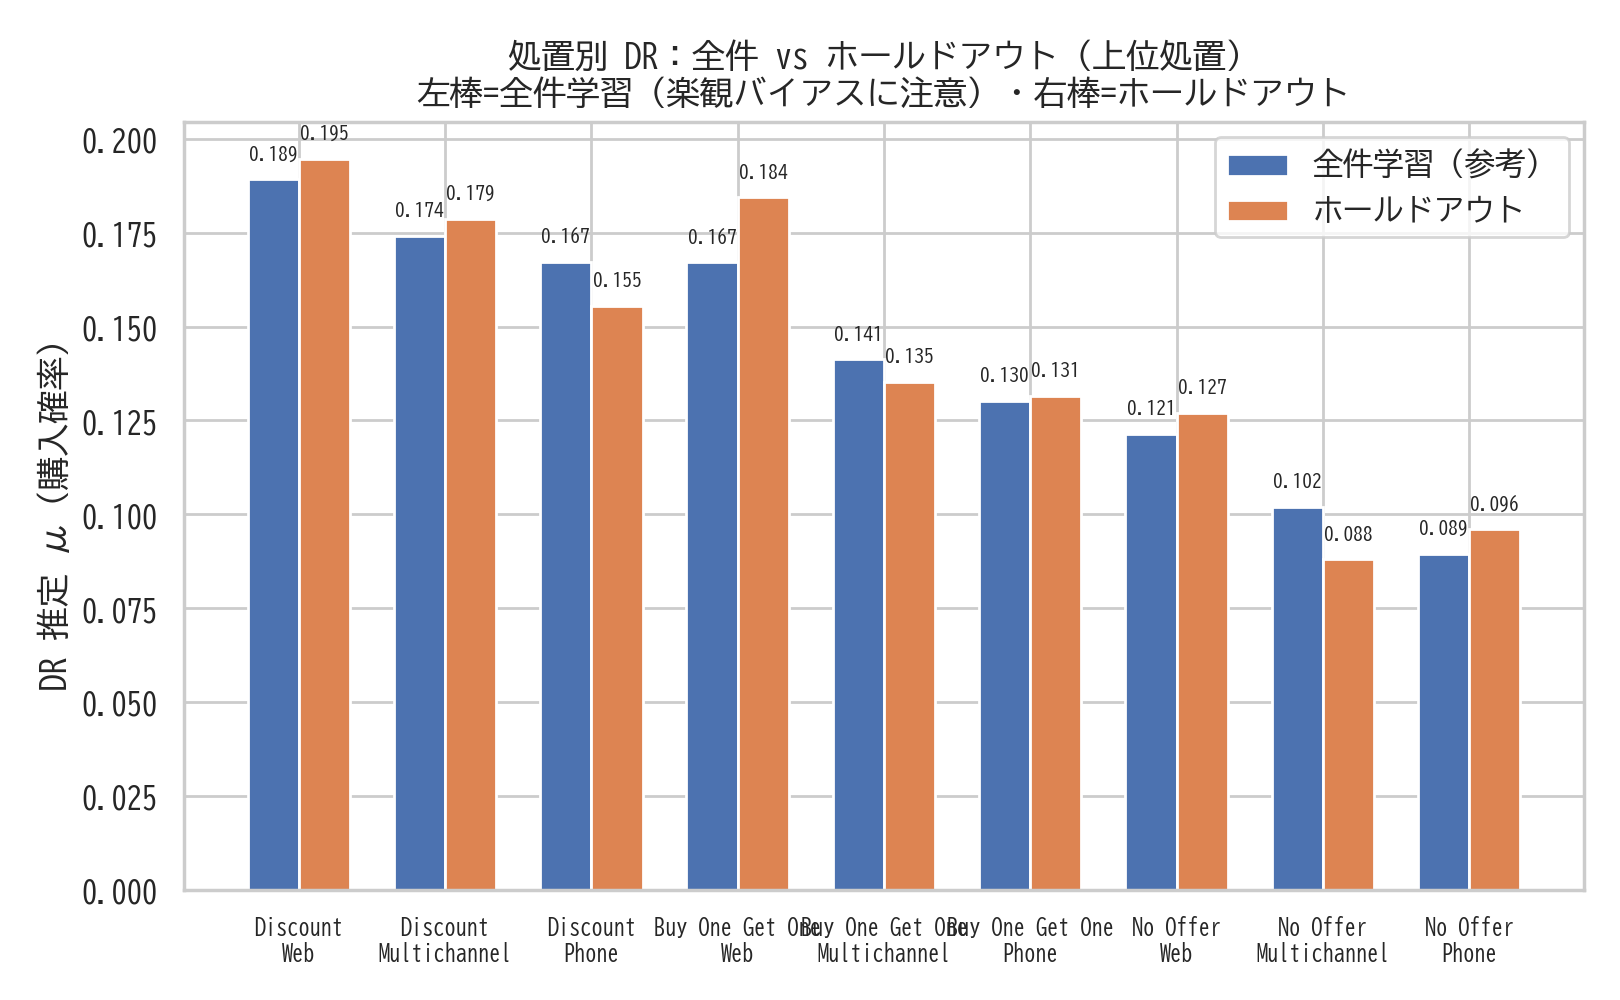
\includegraphics[width=0.92\linewidth]{../figures/improvements/report_dr_full_vs_holdout.png}
  \caption{処置別 DR：全件学習による評価とホールドアウト再学習による評価の比較}
  \label{fig:dr_compare}
\end{figure}

\subsubsection*{解釈}
処置ごとに全件とホールドアウトの差が大きい場合、\textbf{過学習}、\textbf{傾向の極小確率}、
または\textbf{結果モデルの誤指定}が疑われる。差が小さくても\textbf{未観測交絡}は残る。

\begin{figure}[htbp]
  \centering
  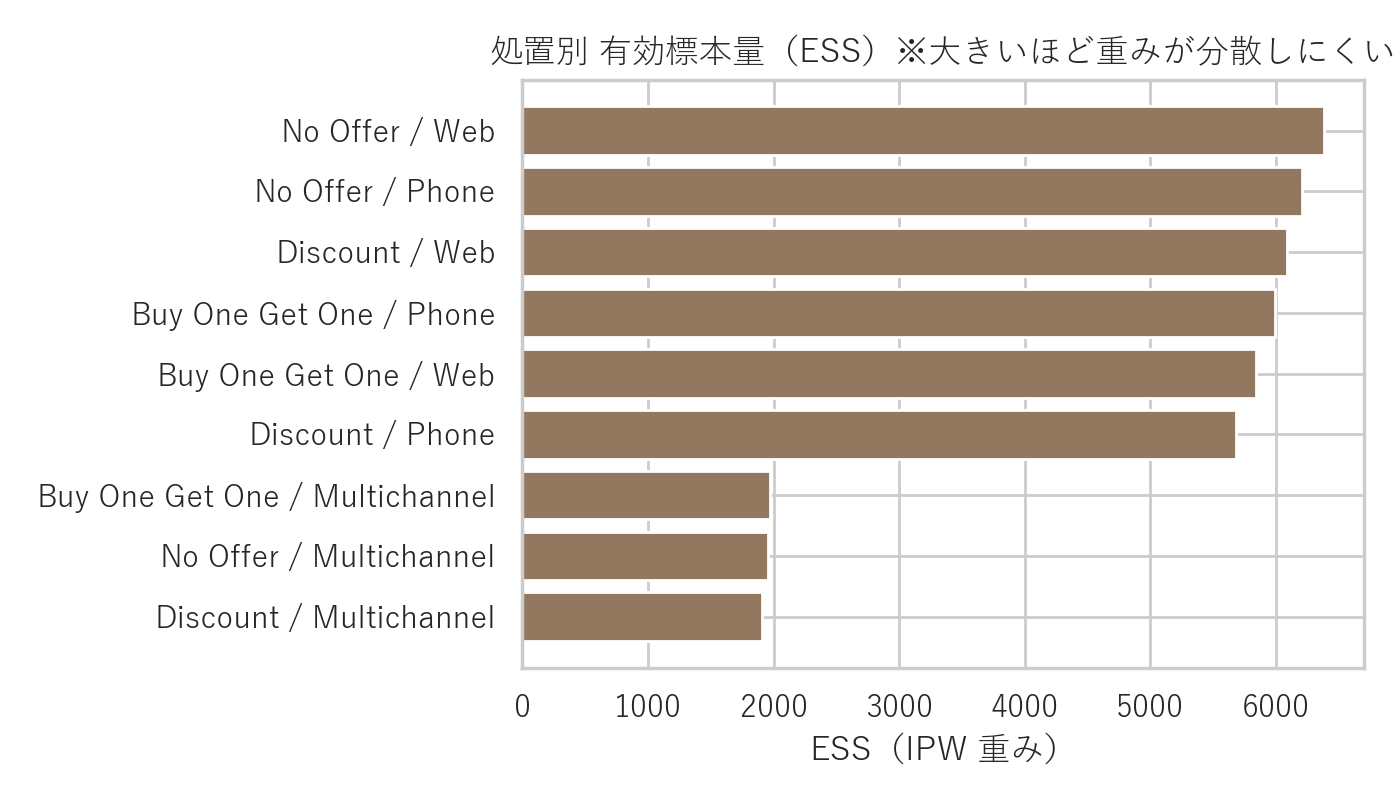
\includegraphics[width=0.85\linewidth]{../figures/improvements/report_propensity_ess.png}
  \caption{処置別 ESS（IPW 重みに対応する有効標本量の目安）}
  \label{fig:ess}
\end{figure}

\subsubsection*{解釈}
ESS が低い処置では、少数観測に過度に重みが乗り、DR の分散が増大する。
その場合、政策の主役から外す・\textbf{傾向のトリミング}（極端に小さい $\hehat$ を持つ単位の除外）・\textbf{処置セルの集約}（類似オファーをまとめて $|\mathcal{T}|$ を縮小）・別母集団での感度分析を検討する。

\begin{figure}[htbp]
  \centering
  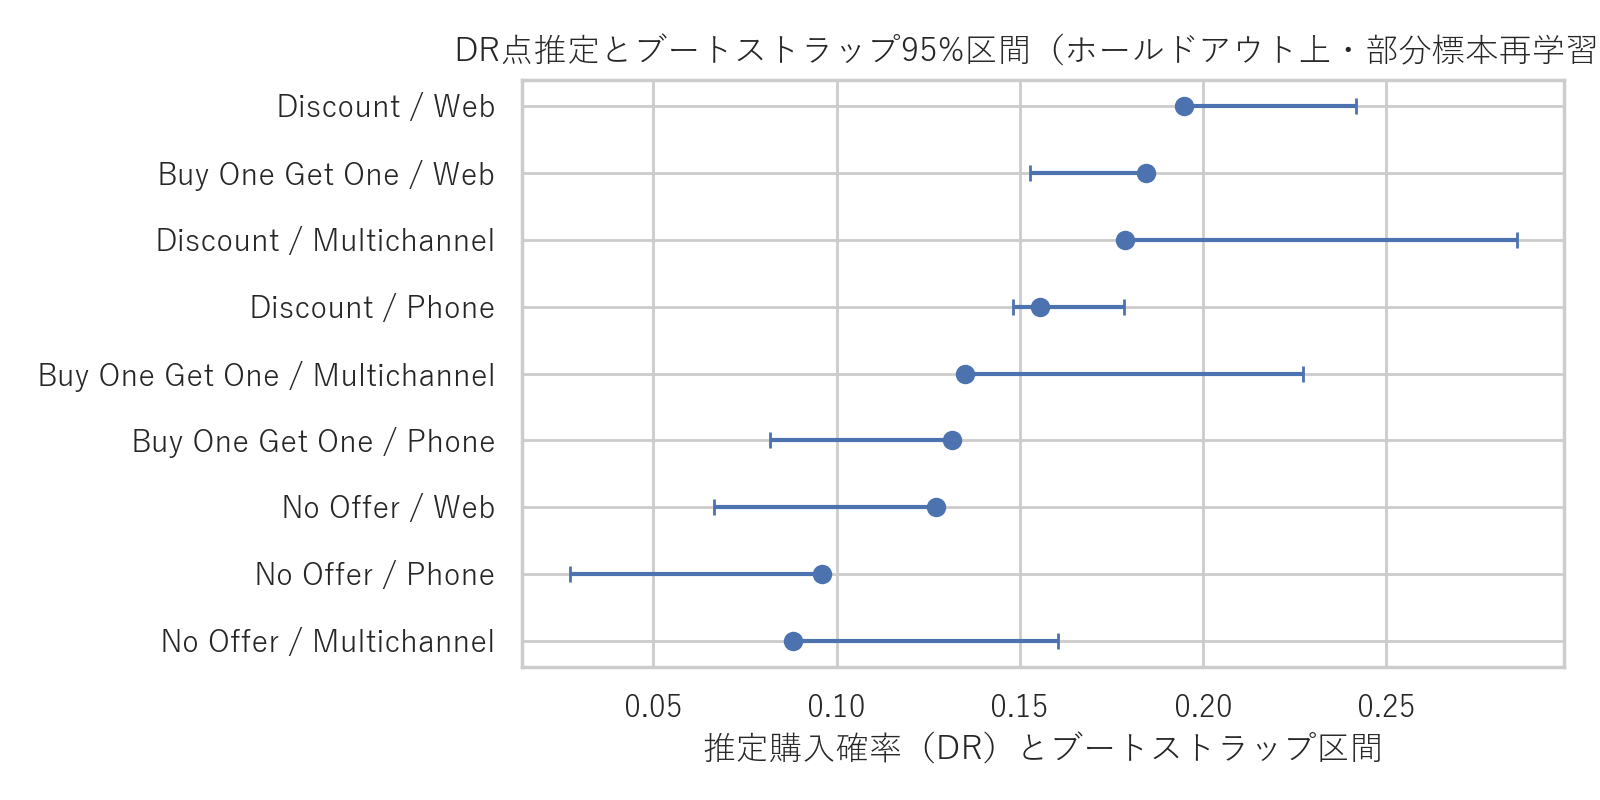
\includegraphics[width=0.75\linewidth]{../figures/improvements/dr_bootstrap_ci.png}
  \caption{DR 点推定とブートストラップ区間（森林図風）}
  \label{fig:dr_boot}
\end{figure}

\subsubsection*{解釈}
区間は\textbf{部分標本再学習}に基づく。処置間で区間が重なるとき、\textbf{順位確定}には実験が有効である。

\subsection{層別の観察差と「無駄割引」仮説への接続（参考）}
観察データのみでは処置の増分効果（uplift）は識別できないが、購入スコアを層別化したうえで\textbf{観察された}オファー間のCVR差を眺めることは\textbf{仮説生成}には有用である。
第\ref{sec:summary_pilot}節の図\ref{fig:uplift_crude_gap}は、スコア十分位ごとに「Discount」と「No Offer」の観察CVR差を示す（\textbf{割当交絡あり}）。
高スコア側で差が相対的に小さい場合は、もともと購入確率が高い層では割引の\textbf{辺際的上乗せ}が小さい可能性を想起させる――いわゆる\textbf{無駄割引}問題だが、確証はRCTが要る\cite{Kohavi2020,Gordon2019}。

\section{期待利益・オフポリシー評価・ベンチマーク}
\label{sec:opeval}

\noindent\textbf{（この節のねらい）}
購入確率だけでなく\textbf{粗利proxyとコスト仮定}を合成し、\textbf{どの処置を誰に送るとオフライン上もっとも良さそうか}を離散政策として評価する。
フル学習とOOFの差は\textbf{過信（楽観バイアス）の目安}になる。
オフポリシー評価・方策学習の理論的整理は \cite{Dudik2011}、オンライン実験の実務は \cite{Kohavi2020} を参照。

\subsection{期待利益の定義（オフライン代理）}
顧客 $i$、処置 $t$ について、本稿で用いる期待利益の代理は
\begin{equation}
  \label{eq:profit}
  \Pihat_i(t)
  = \pihat(t, X_i)\, H_i
  - c_{\mathrm{off}}(t)\, H_i
  - c_{\mathrm{ch}}(t)\, H_i .
\end{equation}
ここで $c_{\mathrm{off}}(t)$、$c_{\mathrm{ch}}(t)$ はシナリオ依存のコスト係数（\texttt{DEFAULT\_SCENARIOS}）。
離散処置について $\arg\max_{t \in \mathcal{T}} \Pihat_i(t)$ を\textbf{個別最適政策}とみなす。

\medskip\noindent
\textbf{コスト仮定の感度（推奨処置の入れ替わり）.}
\texttt{analytics/config.py} の \texttt{low\_cost} / \texttt{mid\_cost} / \texttt{high\_cost} は係数が異なるが、
現行の $\pihat$ のもとでは\textbf{最頻推奨がすべて同一になる}場合がある（コスト項の差が離散最適を変えない）。
そこで \texttt{artifacts/profit\_long.csv} に記録された処置別購入確率と \texttt{history} を固定し、\textbf{より幅の広い係数パターン}で期待利益を再計算した結果を表 \ref{tab:cost_sensitivity_modes} に示す。
極端な設定同士では顧客ごとの最適処置が\textbf{大きく不一致}になりうる――すなわち、\textbf{コスト見積りが政策の結論を左右しうる}ことを示す（あくまでオフライン・参考）。

% auto-generated by scripts/build_cost_sensitivity_from_profit_long.py
\begin{table}[htbp]
  \centering
  \small
  \caption{コストシナリオ別の最頻推奨処置（\texttt{profit\_long.csv} の $p$・\texttt{history} を固定し、係数のみ変更して再計算。参考）}
  \label{tab:cost_sensitivity_modes}
  \begin{tabular}{@{}p{0.42\linewidth}p{0.48\linewidth}r@{}}
    \toprule
    シナリオ（概略） & 最頻推奨（処置） & 割合 \\
    \midrule
    extreme\_lean（割引係数小） & \texttt{Discount / Web} & 86.1\% \\
    low\_cost（config 相当・やや控えめ） & \texttt{No Offer / Web} & 96.3\% \\
    mid\_cost & \texttt{No Offer / Web} & 100.0\% \\
    high\_cost & \texttt{No Offer / Web} & 100.0\% \\
    extreme\_heavy（割引係数大） & \texttt{No Offer / Web} & 100.0\% \\
    \bottomrule
  \end{tabular}
\medskip
  \par\noindent\footnotesize 極端設定間（\texttt{extreme\_lean} vs \texttt{extreme\_heavy}）で\textbf{同一の離散処置}が選ばれた顧客の割合：\textbf{13.9\%}（残りは処置が不一致＝コスト仮定で結論が入れ替わる）。
\end{table}


\subsection{オフポリシー評価の読み方}
\textbf{フル学習}: 全データで学習した $\pihat$ で評価（楽観バイアスがありうる）。
\textbf{OOF}: $K$折で学習していないフォールドの予測を用いる。
\textbf{ホールドアウト}: 保持検証セット上の予測を用いる。

\begin{figure}[htbp]
  \centering
  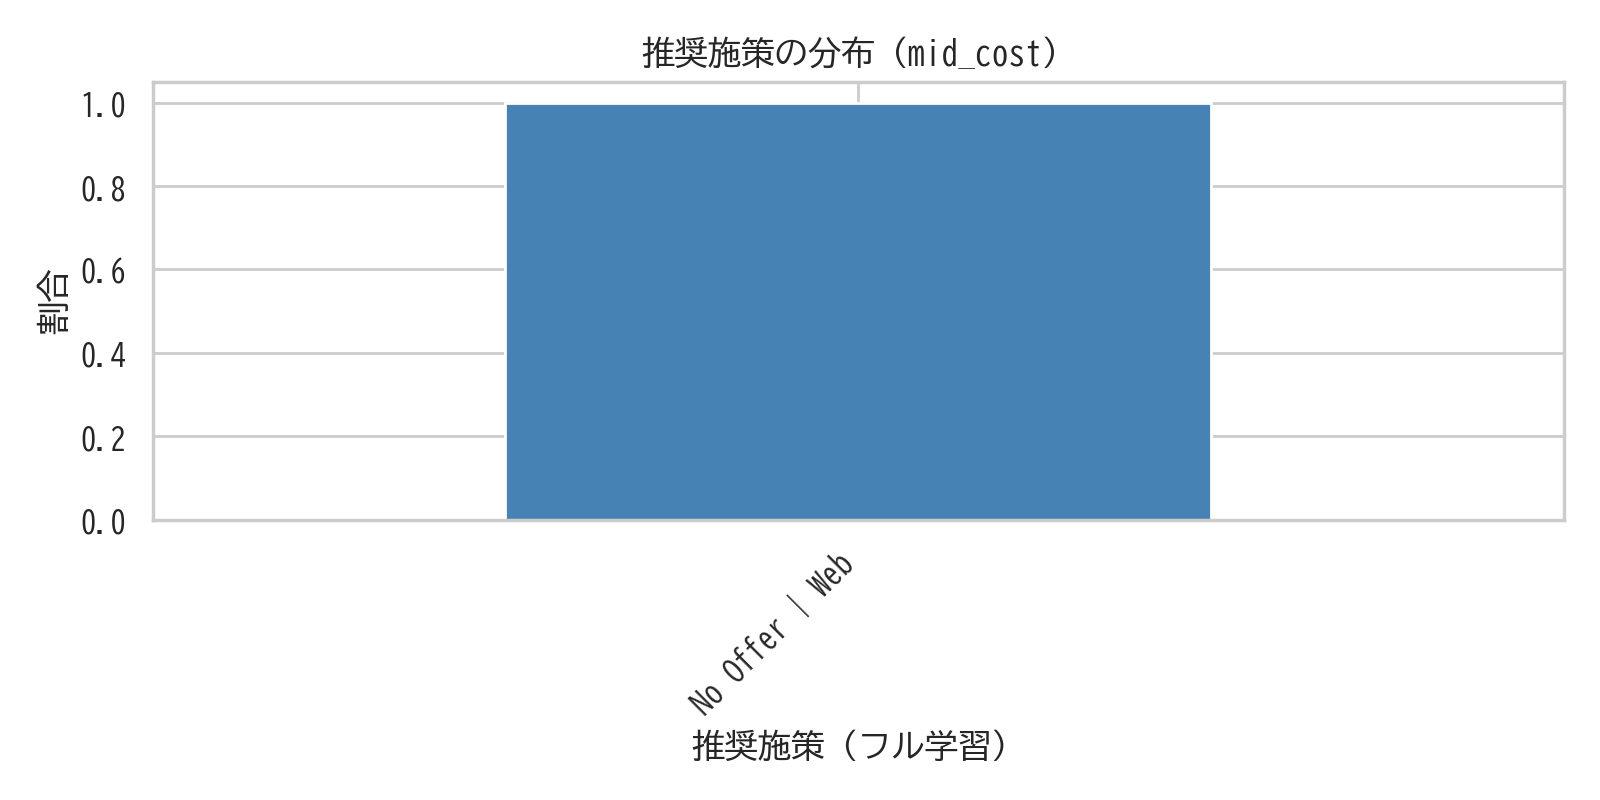
\includegraphics[width=0.88\linewidth]{../figures/improvements/policy_reco_dist_full.png}
  \caption{推奨処置の分布（シナリオ別）}
  \label{fig:policy_reco}
\end{figure}

\begin{figure}[htbp]
  \centering
  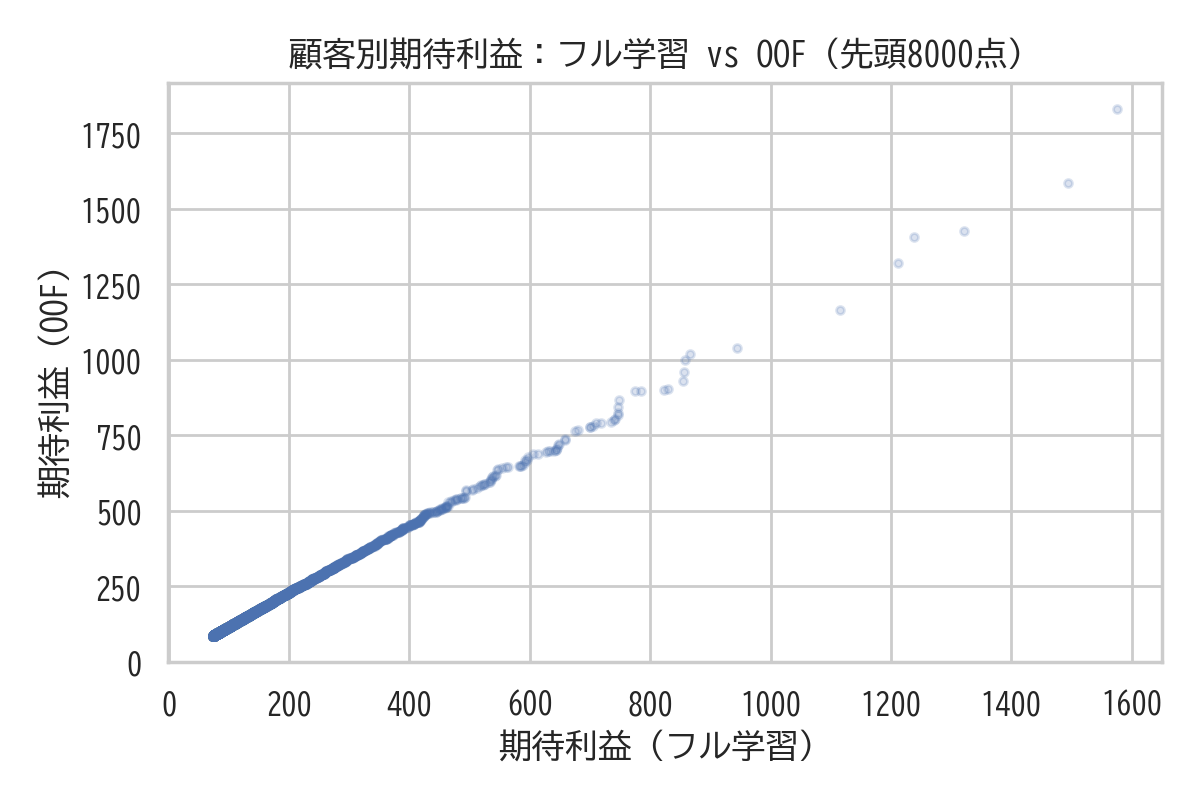
\includegraphics[width=0.88\linewidth]{../figures/improvements/profit_full_vs_oof_scatter.png}
  \caption{フル学習 vs OOF 期待利益（顧客ごと）}
  \label{fig:profit_scatter}
\end{figure}

\begin{figure}[htbp]
  \centering
  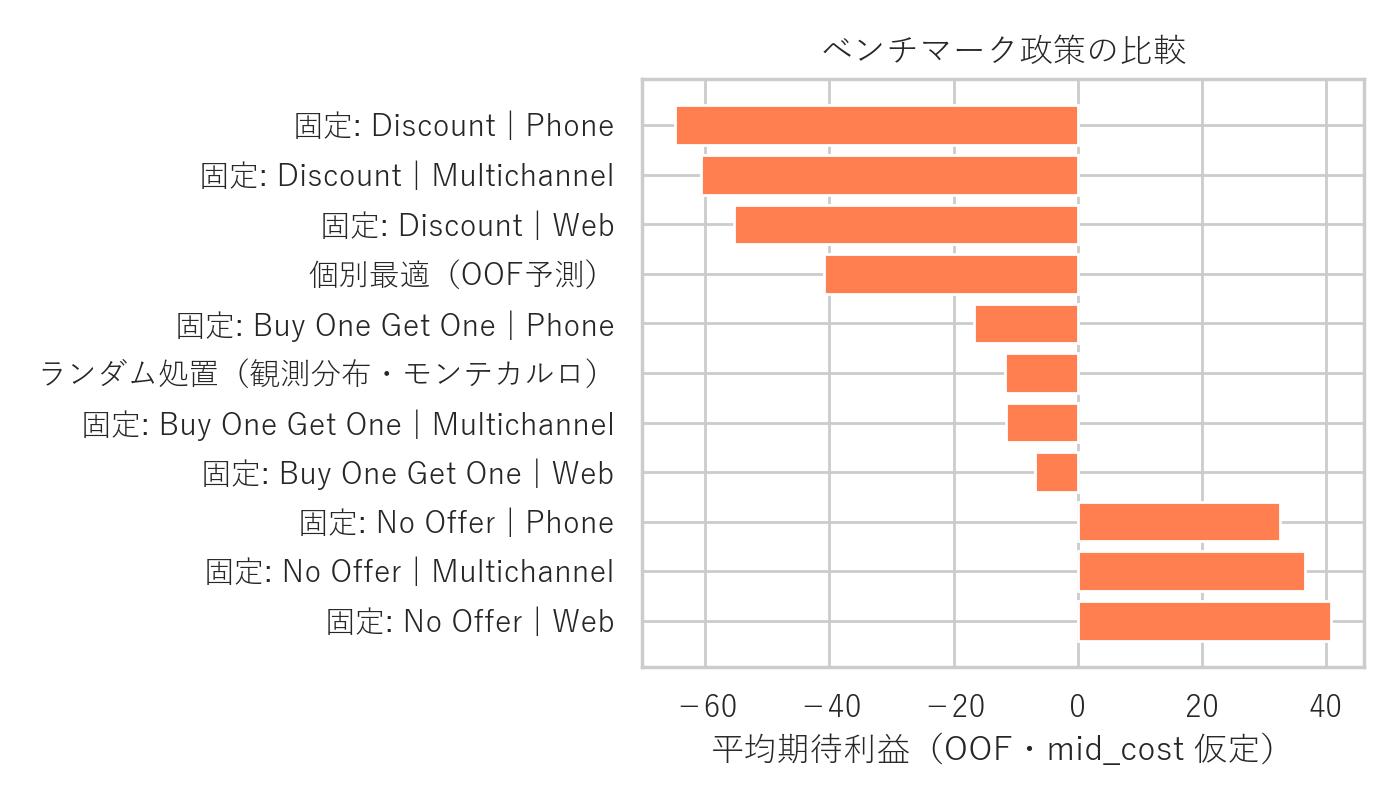
\includegraphics[width=0.88\linewidth]{../figures/improvements/policy_benchmarks_bar.png}
  \caption{ベンチマーク政策の比較}
  \label{fig:policy_bench}
\end{figure}

\begin{figure}[htbp]
  \centering
  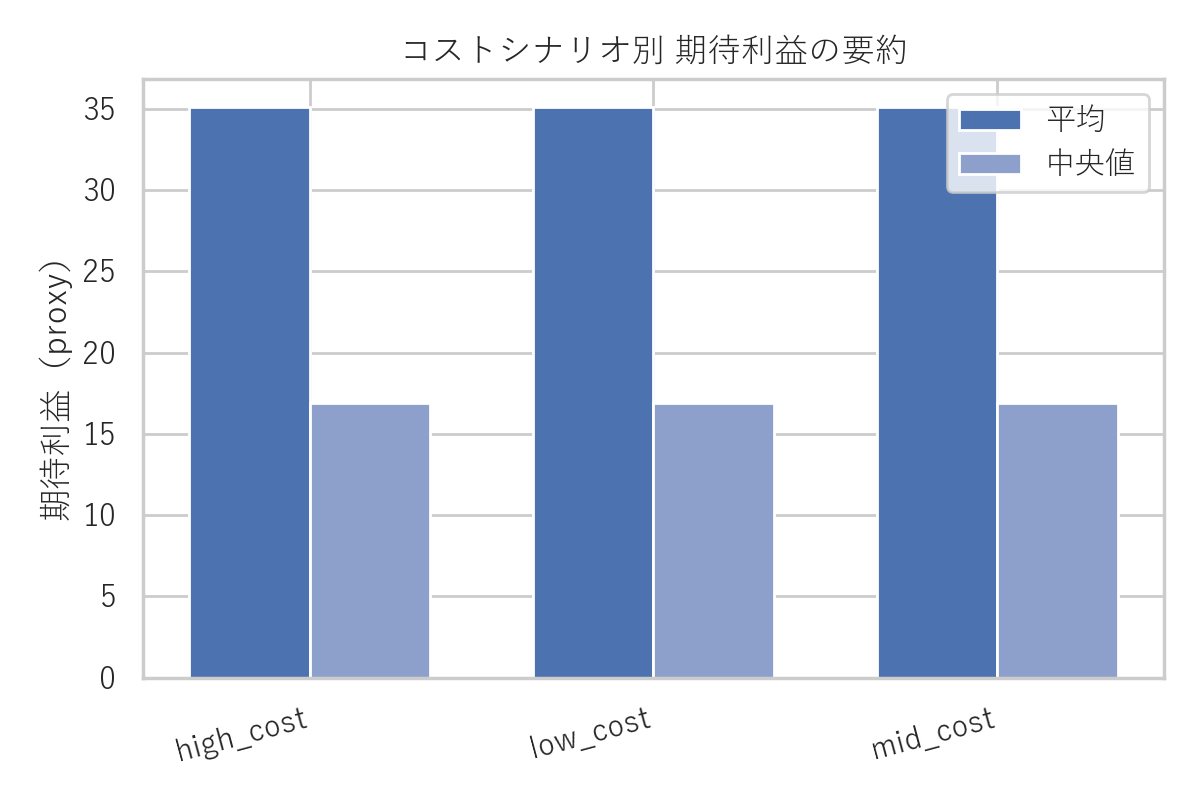
\includegraphics[width=0.88\linewidth]{../figures/improvements/report_profit_summary_by_scenario.png}
  \caption{シナリオ別 期待利益要約}
  \label{fig:profit_summary}
\end{figure}

\subsubsection*{解釈}
推奨分布の集中（例：一処置に100\%）は、\textbf{コスト仮定のもとで他処置が支配的に不利}なことの\textbf{シグナル}であるが、
モデル誤差でも起こりうるため散布図と OOF を併読する。
ベンチマーク棒は\textbf{単純ルールで十分か}の基準線を与える。

\begin{figure}[htbp]
  \centering
  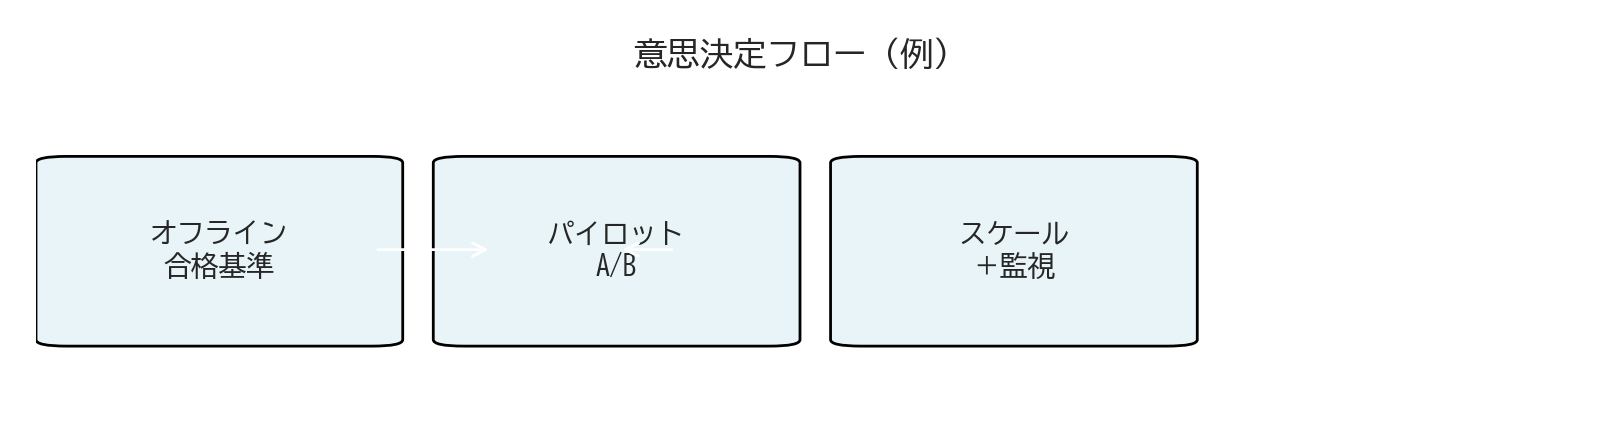
\includegraphics[width=0.88\linewidth]{../figures/improvements/decision_flow.png}
  \caption{意思決定フロー（ゲート例）}
  \label{fig:decision_flow}
\end{figure}

\begin{figure}[htbp]
  \centering
  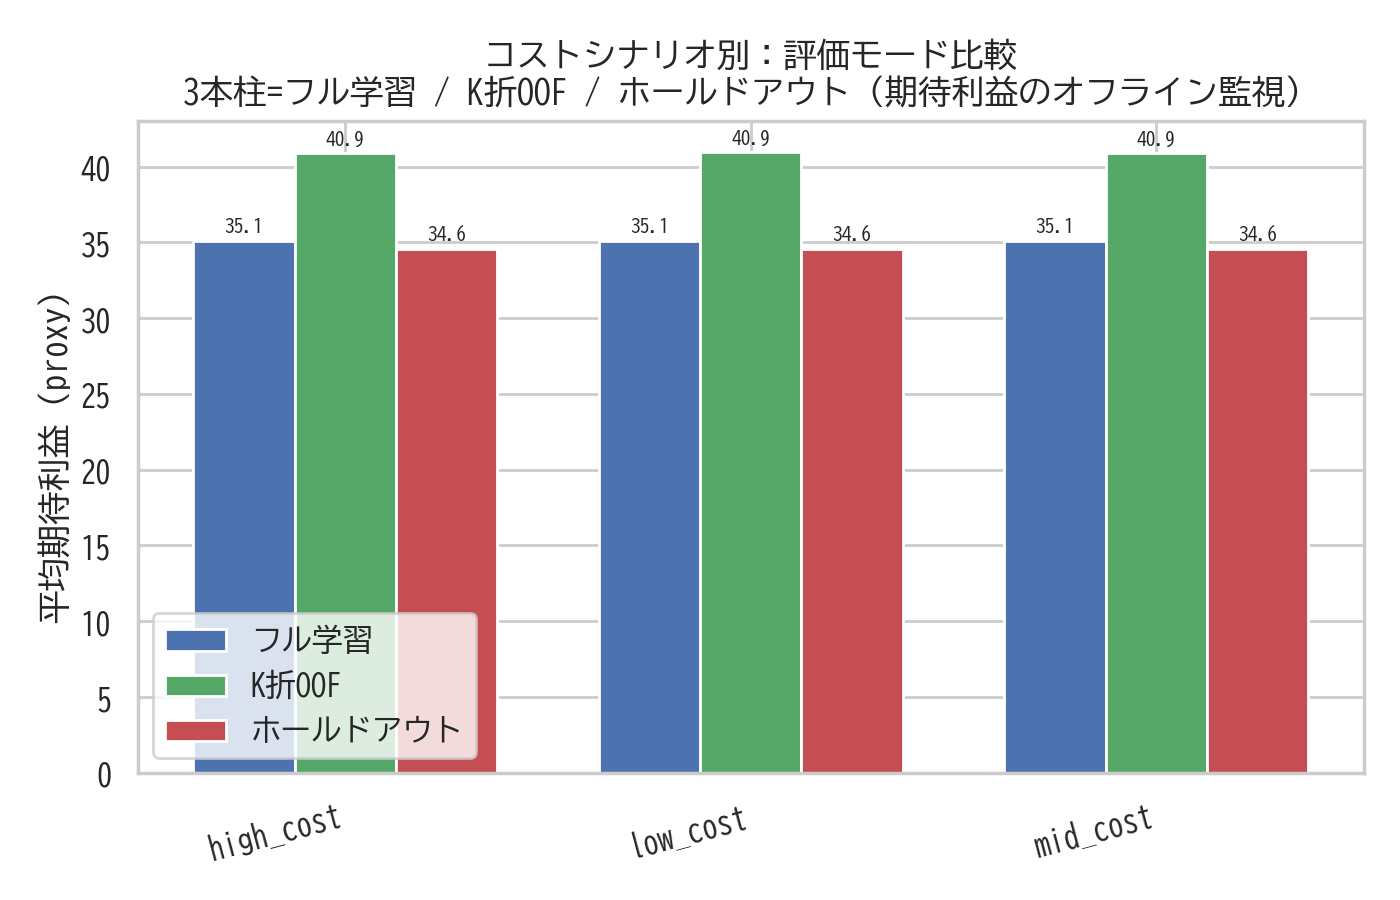
\includegraphics[width=0.88\linewidth]{../figures/improvements/report_policy_eval_means.png}
  \caption{評価モード別 平均期待利益}
  \label{fig:policy_eval_means}
\end{figure}

\subsubsection*{解釈}
図 \ref{fig:decision_flow} は\textbf{オフライン合格 $\rightarrow$ パイロット $\rightarrow$ スケール}の例。
図 \ref{fig:policy_eval_means} でフルだけ突出していれば、\textbf{過信}の警告となる。

\subsection{制約付き配信（貪欲近似）}
接触上限・予算等の\textbf{整数制約}下では、全員への $\arg\max_{t}$ は実行不可能な場合がある。
実装では貪欲割当により\textbf{近似解}を求める。一般に\textbf{最適解との最適性ギャップ}は問題依存である。

\begin{figure}[htbp]
  \centering
  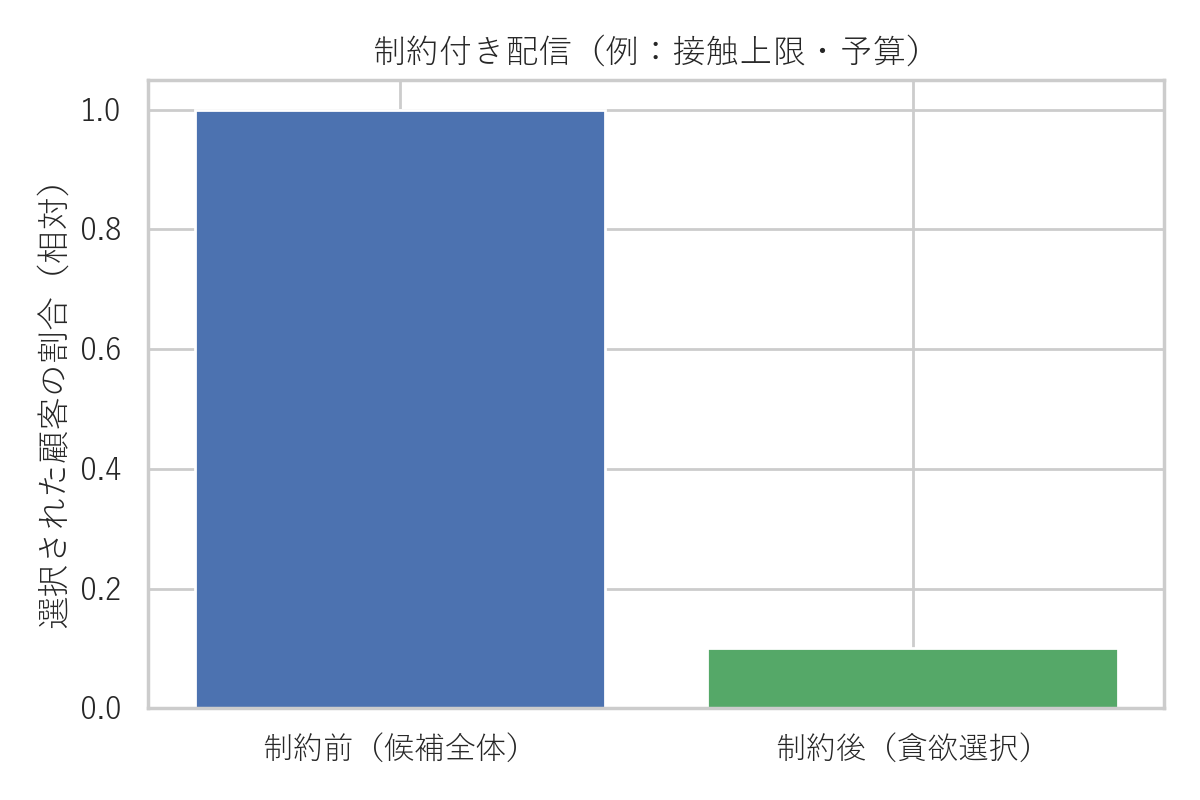
\includegraphics[width=0.65\linewidth]{../figures/improvements/constrained_selection_summary.png}
  \caption{制約付き配信：選択割合の変化（例）}
  \label{fig:constrained}
\end{figure}

\subsubsection*{解釈}
図は\textbf{運用イメージ}であり、実予算・キャパに合わせパラメータを再設定する。
完全最適が必要な場合は MIP 等との比較が望ましい。

\section{セグメントと頑健性}
\label{sec:segment}

\noindent\textbf{（この節のねらい）}
顧客を\textbf{類似した群}に分け、施策メッセージや検証単位のイメージを掴む。
クラスタの安定性（ARI）が低いときは、セグメント固定ルールの再現性に注意する。

\subsection{潜在空間の可視化}
PCA は線形、UMAP は非線形構造を強調するが、\textbf{大域的距離の厳密解釈は持たない}。
クラスタリングは主に UMAP 座標上で実施し、\textbf{ARI} でシード頑健性を確認する。

\begin{figure}[htbp]
  \centering
  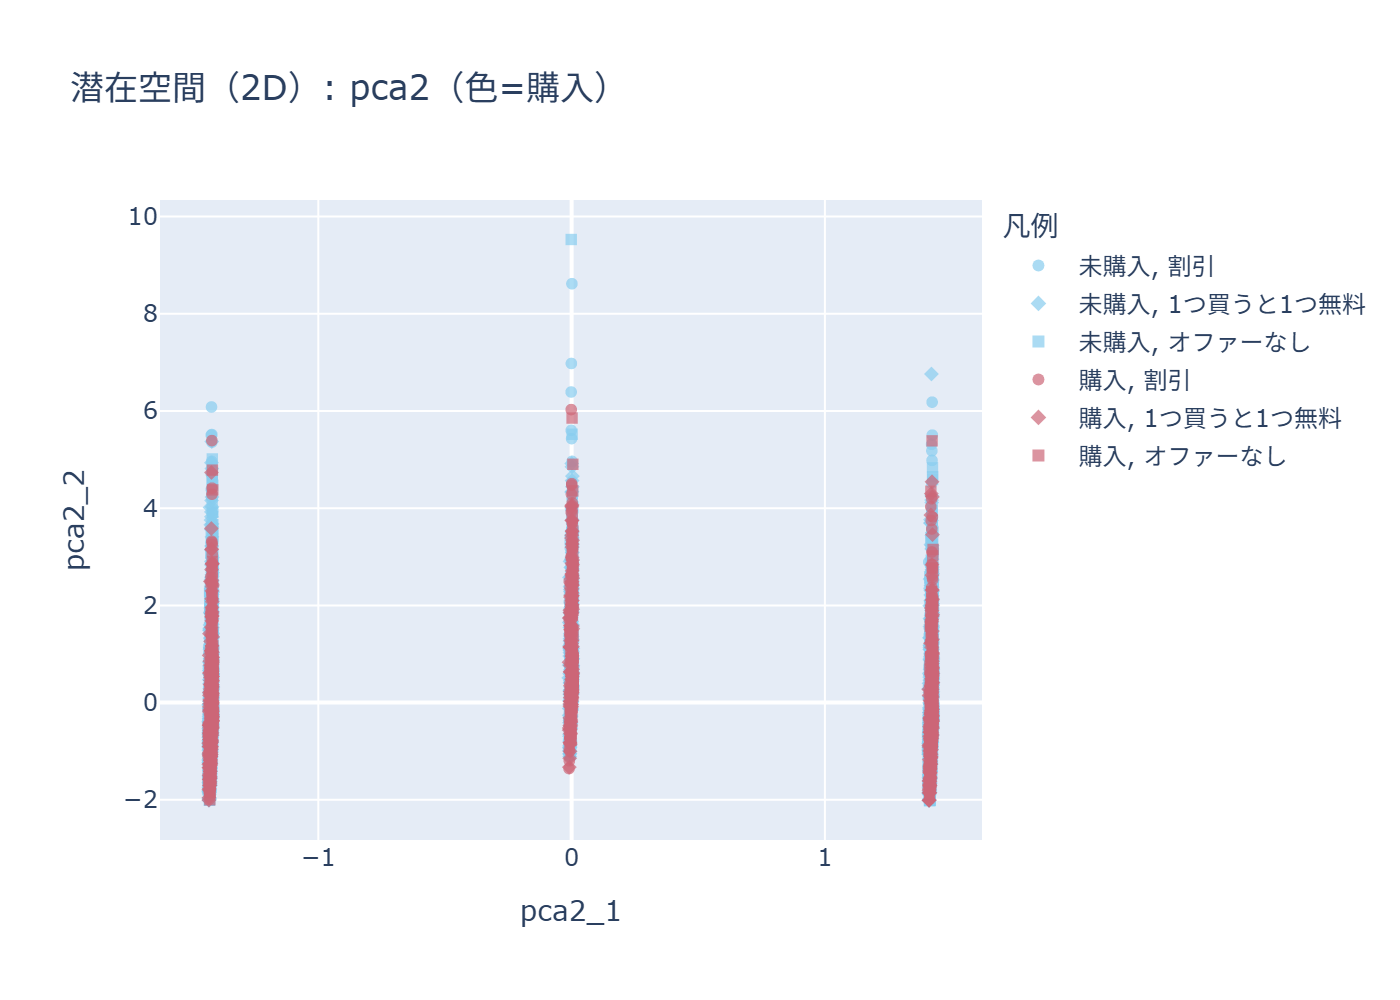
\includegraphics[width=0.88\linewidth]{../figures/improvements/latent2d_pca2_color_conversion.png}
  \caption{潜在空間：PCA 2D（購入で色分け）}
  \label{fig:latent_pca2}
\end{figure}

\begin{figure}[htbp]
  \centering
  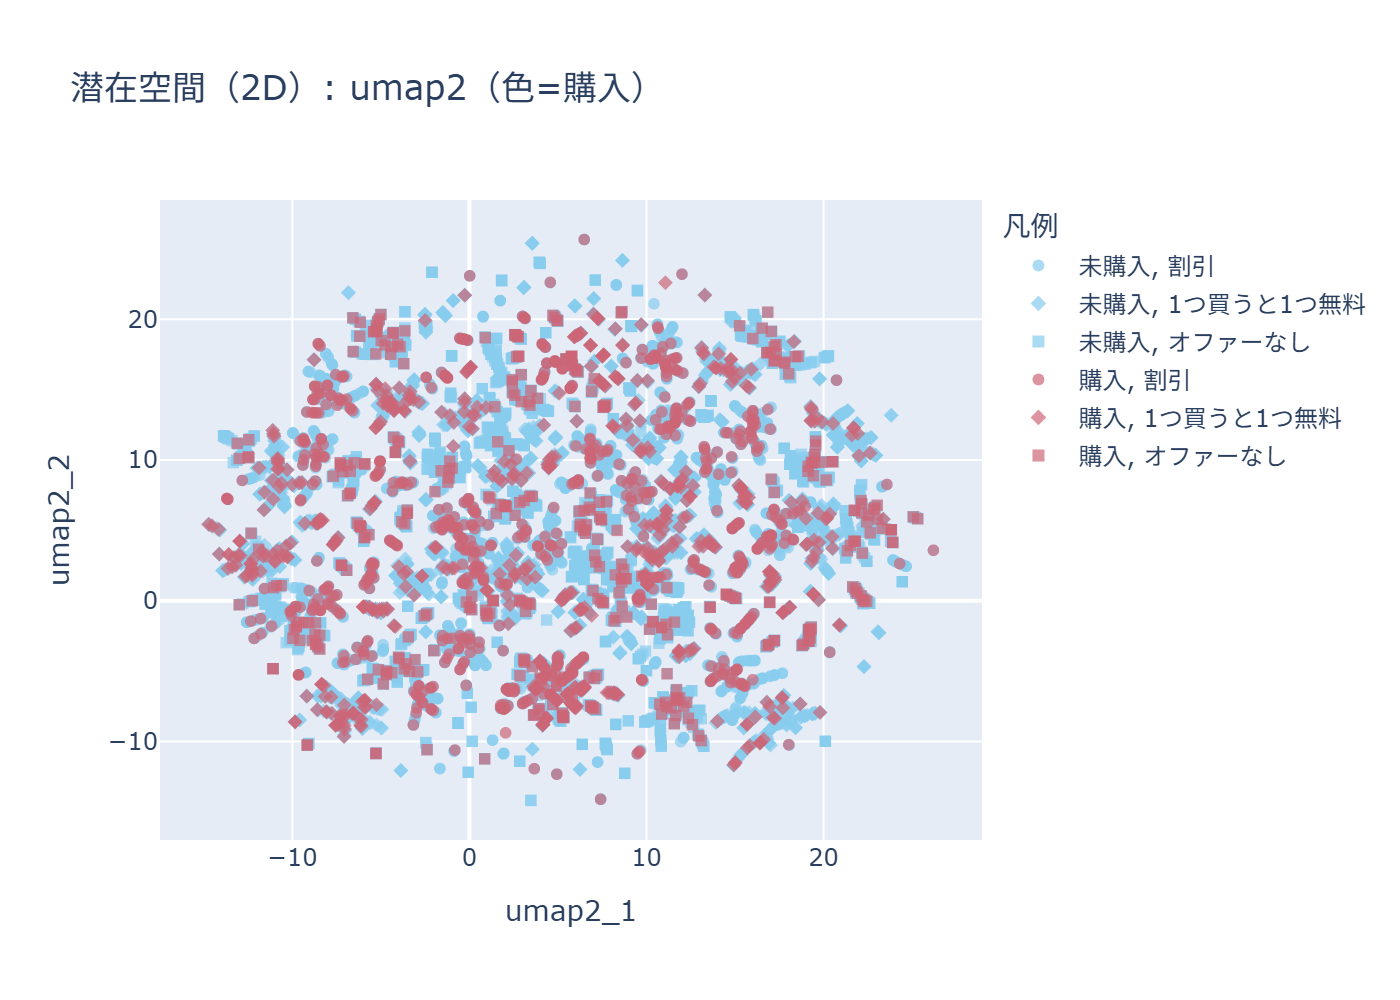
\includegraphics[width=0.88\linewidth]{../figures/improvements/latent2d_umap2_color_conversion.png}
  \caption{潜在空間：UMAP 2D}
  \label{fig:latent_umap2}
\end{figure}

\begin{figure}[htbp]
  \centering
  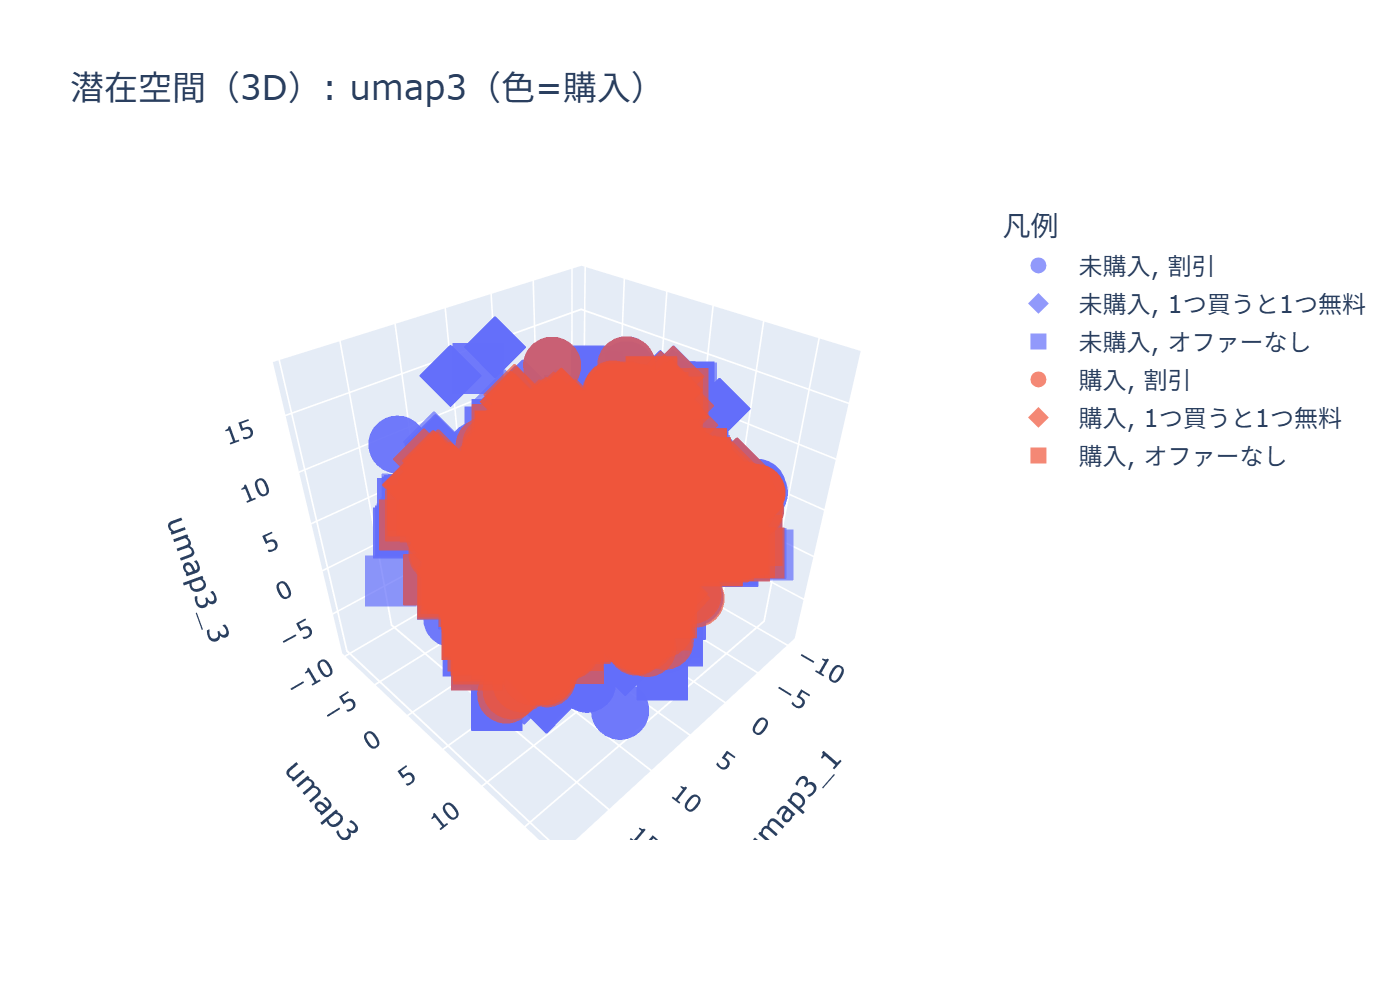
\includegraphics[width=0.88\linewidth]{../figures/latent3d_umap3_color_conversion.png}
  \caption{潜在空間：UMAP 3D（PNG 静止画）}
  \label{fig:latent_umap3}
\end{figure}

\begin{figure}[htbp]
  \centering
  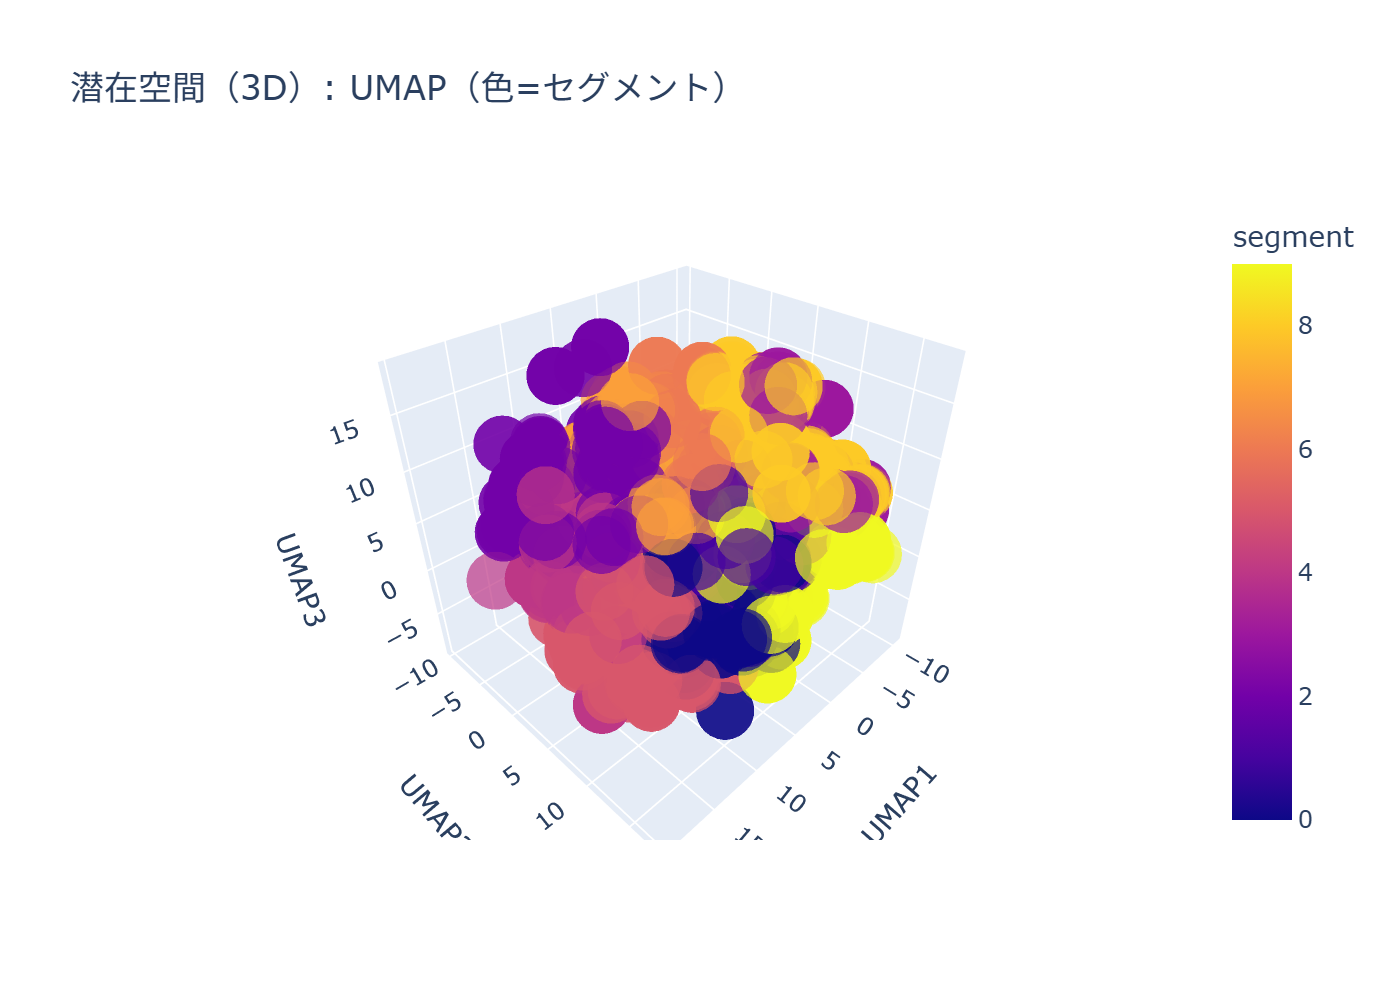
\includegraphics[width=0.88\linewidth]{../figures/improvements/latent3d_umap3_color_segment.png}
  \caption{潜在空間：セグメント着色（UMAP 3D）}
  \label{fig:latent_seg}
\end{figure}

\subsubsection*{解釈}
セグメントラベルは\textbf{説明用}であり、差別的利用やセンシティブ属性の proxy 化には\textbf{人のレビュー}を要する。
HTML 版は \texttt{figures\_html/} を参照。

\begin{figure}[htbp]
  \centering
  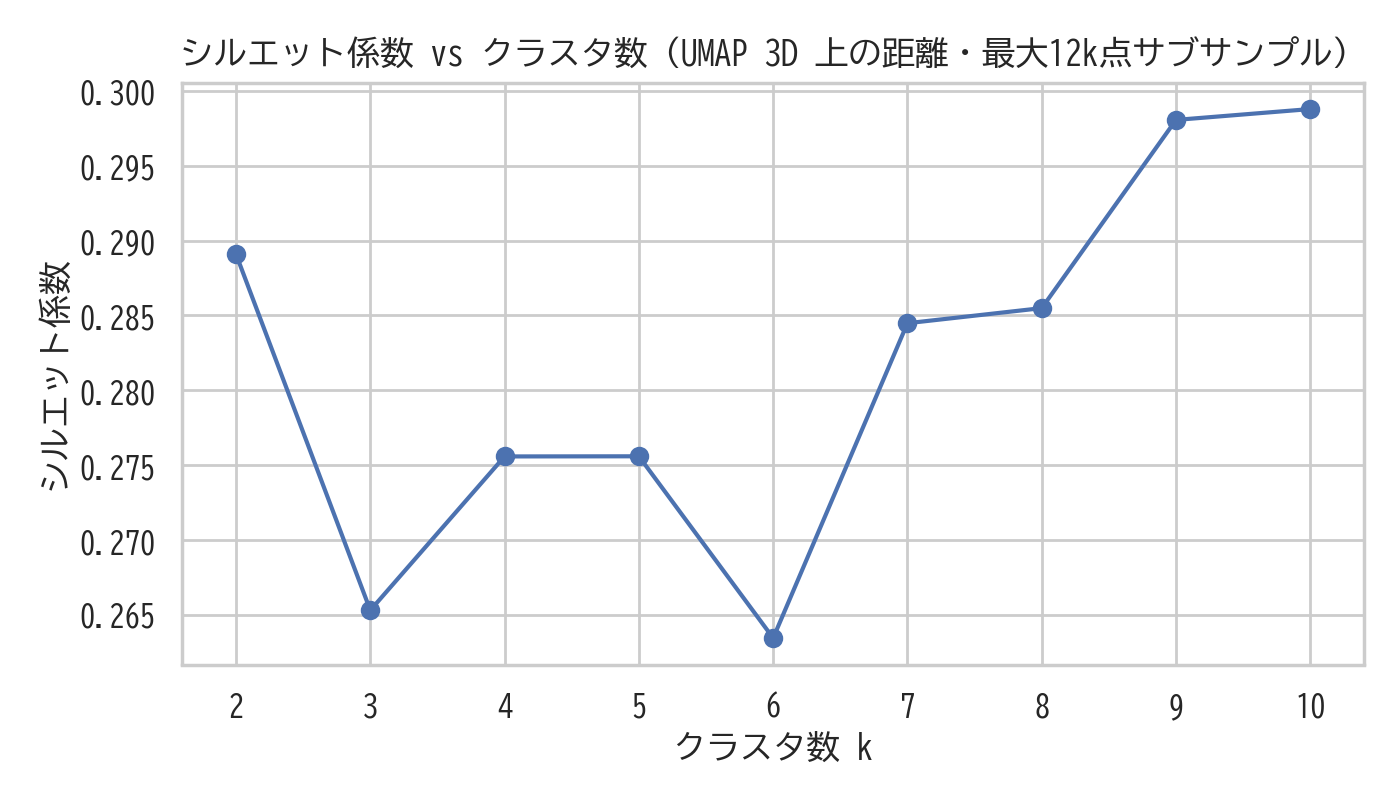
\includegraphics[width=0.88\linewidth]{../figures/improvements/silhouette_vs_k.png}
  \caption{クラスタ数 $k$ とシルエット係数}
  \label{fig:silhouette}
\end{figure}

\begin{figure}[htbp]
  \centering
  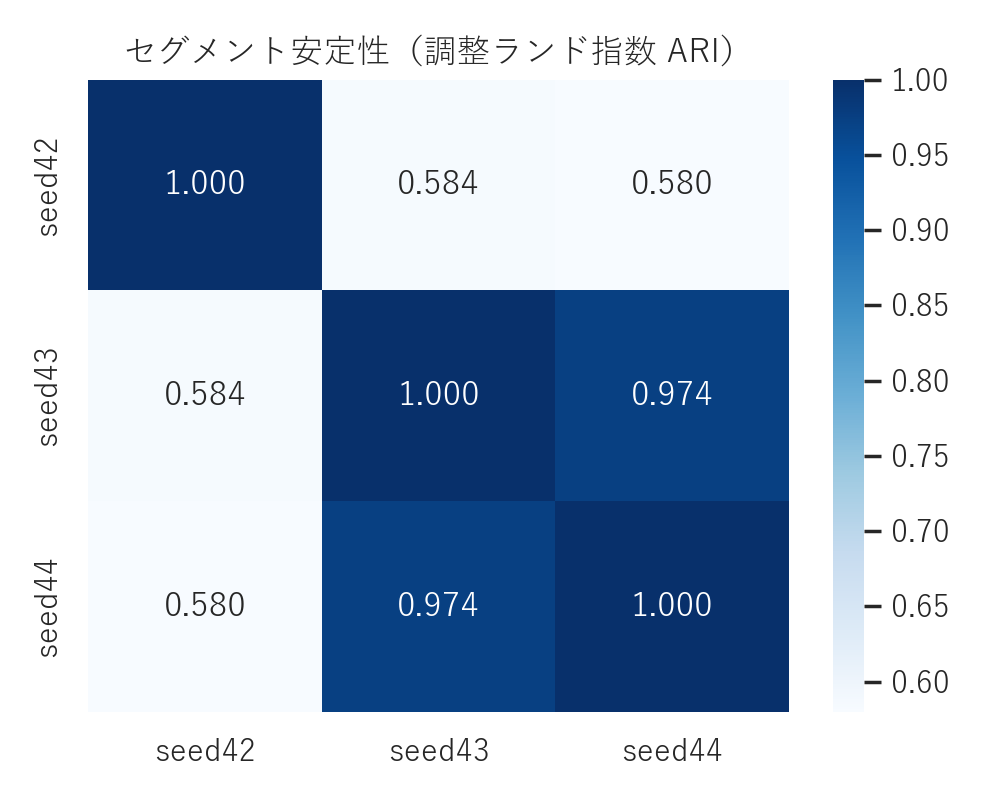
\includegraphics[width=0.88\linewidth]{../figures/improvements/segment_stability_ari.png}
  \caption{多シードに対するクラスタ安定性（ARI）}
  \label{fig:ari}
\end{figure}

\subsubsection*{解釈}
ARI が低い場合、セグメント施策の固定化は\textbf{再現性リスク}を伴う。スコア層への回帰や合意クラスタを検討する。

\subsection{セグメント$\times$処置の観測CVR（探索）}
図 \ref{fig:seg_treat} は UMAP セグメントと処置（オファー$\times$チャネル）の組み合わせにおける\textbf{観測CVR}を示す。
交絡があるため因果効果の読み替えはできない（記述のみ）。詳細は \texttt{artifacts/segment\_treatment\_cvr\_exploratory.csv}。

\begin{figure}[htbp]
  \centering
  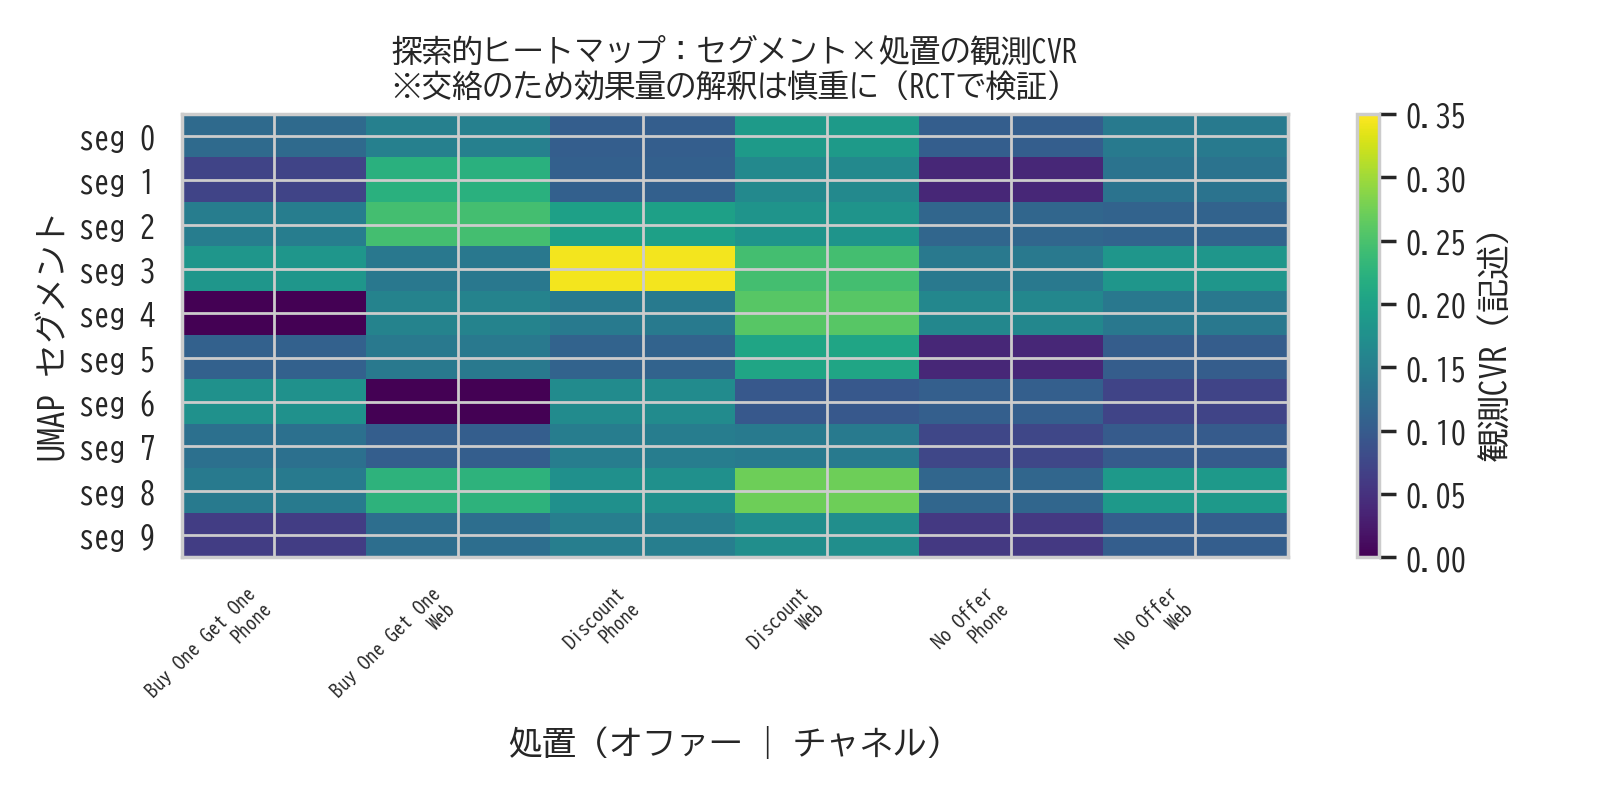
\includegraphics[width=0.92\linewidth]{../figures/improvements/segment_treatment_cvr_heatmap_exploratory.png}
  \caption{探索的ヒートマップ：セグメント$\times$処置の観測CVR}
  \label{fig:seg_treat}
\end{figure}

\begin{figure}[htbp]
  \centering
  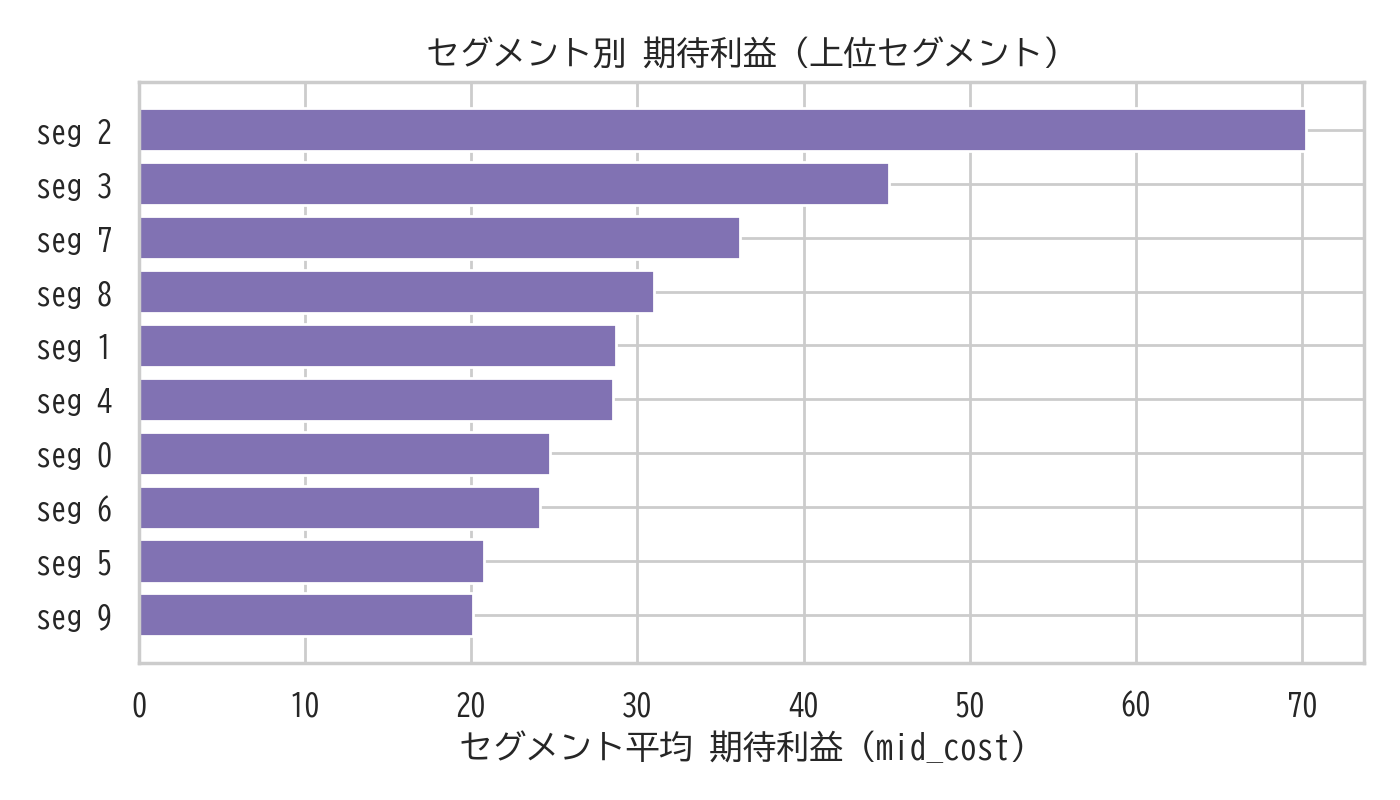
\includegraphics[width=0.75\linewidth]{../figures/improvements/report_segment_mean_profit.png}
  \caption{セグメント別 平均期待利益（参考）}
  \label{fig:seg_profit}
\end{figure}

\subsubsection*{解釈}
棒はクラスタ内平均であり、\textbf{クラスタ人数}と併読する。小クラスタは偶然の振れが大きい。

\section{実験計画（RCT/A/B）}
\label{sec:rct}
主アウトカムを購入率と置き、有意水準・検定力・最小検出効果（MDE）に基づく必要サンプルは表 \ref{tab:ab}。
設計の実務的ガイドは \cite{Kohavi2020}、大規模場における増分計測の比較議論は \cite{Gordon2019} が参考になる。
\begin{table}[ht]
\centering
\caption{A/B 必要サンプル（二標本比例・正規近似）}
\label{tab:ab}
\small
\begin{tabular}{rrrr}
\toprule
MDE & 検定力 & 片群n（近似） & 合計n（近似） \\
\midrule
0.005 & 0.8 & 79742 & 159483 \\
0.005 & 0.9 & 106751 & 213501 \\
0.010 & 0.8 & 20209 & 40418 \\
0.010 & 0.9 & 27054 & 54107 \\
0.015 & 0.8 & 9103 & 18205 \\
0.015 & 0.9 & 12185 & 24370 \\
0.020 & 0.8 & 5187 & 10374 \\
0.020 & 0.9 & 6944 & 13887 \\
\bottomrule
\end{tabular}

\end{table}

\subsubsection*{解釈}
表の $n$ は\textbf{近似の出発点}である。無効検査、多重主アウトカム、クラスタランダム化等で設計を調整する。
オフラインで有効に見えた政策が実験で再現しない場合、\textbf{実装差・SUTVA・残存交絡}を疑う。

\section{ガバナンス・倫理・人の関与}
\label{sec:governance}
\paragraph{目的限定と最小化}
分析目的に必要な列のみを用い、保存期間・アクセス権は社内規程に従う（詳細は \texttt{data\_dictionary.md}）。

\paragraph{説明可能性と人の関与}
セグメント別施策はモデル出力に基づくが、最終配信判断には担当者レビューを置く。自動化された決定のみで不利益を生じさせない運用を推奨。

\paragraph{差別・不利益リスク}
地域（\texttt{zip\_code} 等）などのプロキシ特性に依存する政策は、属性に基づく不当な差別に繋がらないよう設計・監査する。

\paragraph{オプトアウト・問い合わせ}
マーケティング配信の拒否・個人情報の開示等の請求手続きは、社内ポリシーおよび個人情報保護法（日本）の枠組みに従う。

\paragraph{法的助言ではない}
本稿・生成テンプレは\textbf{法的助言を構成しない}。実装・運用前に法務・DPO と整合を取ること。


\section{運用モニタリングとインシデント対応}
\begin{table}[ht]
\centering
\caption{監視指標の例（詳細は \texttt{artifacts/monitoring\_spec.*}）}
\small
\begin{tabular}{ll}
\toprule
領域 & 監視例 \\
\midrule
校正 & Brier / ECE 週次 \\

ドリフト & PSI / KS \\

傾向スコア & ESS・極小e割合 \\

\bottomrule
\end{tabular}

\end{table}

\subsubsection*{解釈}
閾値は組織で合意し、逸脱時の\textbf{縮小運用・再学習・ロールバック}を手順化する。

\section{まとめと今後の方針}

\noindent\textbf{ゴールへの3行（課題の問い：誰にプロモを打つか）.}
\textbf{(1)}~購入確度が高い層は、予測スコア上位に \texttt{history} や紹介などのパターンが現れやすい。
\textbf{(2)}~オフライン期待利益では \textbf{インセンティブを掛けない接触（例：\texttt{No Offer / Web}）}が主軸になりうる――「高確度だから割引」は必ずしも最適ではない。
\textbf{(3)}~次は \textbf{上位スコア層を母集団にしたパイロット実験}で、購入率・利益 proxy（円）・コストを検証する（表 \ref{tab:ab} の母数は出発点）。

\subsection{最終課題の再確認}
課題は、店舗顧客データに基づき\textbf{コンバージョン確度の高いユーザーの傾向}を捉え、
\textbf{プロモーションを打つべき顧客層}を検討し、\textbf{新施策}につなげることであった。
本稿ではこれに答えるため、(1)~\texttt{exercise.csv} に対するEDAと購入予測、(2)~処置別の参考推定と期待利益、(3)~実験・ガバナンスまでを一連の流れとして整理した。

\subsection{分析結果の要約}
\begin{itemize}
  \item \textbf{傾向}：条件付きCVR・予測モデル・セグメント要約から、購入しやすい層は \texttt{history} や紹介などの信号と整合的なパターンを示す（ただし交絡あり）。
  \item \textbf{ターゲティング}：スコア上位（Top K\%）は実測CVRがベースレートを上回り、\textbf{接触枠の配分}には使える。
  \item \textbf{政策}：期待利益のオフライン代理では、コスト仮定によっては\textbf{無オファー・Web等が支配的}になりうる。オフライン合格後はRCTで増分効果を確認するのが筋である。
\end{itemize}

\subsection{想定や直感と異なる結果とその理由}
課題の字面だけでは「購入確度が高い人にプロモを打つ」ことが最適に読めるが、本データと目的関数では次のように\textbf{読み替え}が必要である。
\begin{itemize}
  \item \textbf{購入しそうな人への割引は利益が出にくい}：購入確率が高くても、インセンティブコストを引くと期待利益は低くなりうる（\textbf{増分性}は別問題だが、期待利益最大化はその方向を示す）。
  \item \textbf{記述CVRが高いオファーが全体最適とは限らない}：観察された割当のもとでの条件付き頻度であり、かつコスト項で逆転しうる。
  \item \textbf{オフライン最適は過信しうる}：同一データで学習したモデルでの評価は楽観的になりやすい。OOF・ホールドアウト・ESSで様子を見る。
\end{itemize}

\subsection{今後の方針（新施策の提案）}
\begin{itemize}
  \item \textbf{パイロット設計}：上位スコア層（例：Top 5--10\%）を母集団に、\textbf{低コスト訴求 vs 現行オファー vs ホールドアウト}の二因子程度から開始し、購入率・利益proxy・接触コストを同時に見る（第\ref{sec:rct}節のサンプルは出発点）。
  \item \textbf{副次アウトカム}：試験終了後\textbf{90日}の累積売上（またはLTV proxy）と\textbf{90日以内再購入}を事前登録し、短期CVR改善が長期価値を損なわないか監視する（表\ref{tab:kpi_hierarchy}）。
  \item \textbf{運用ゲート}：校正ドリフト・PSI・ESS・OOFとのギャップが閾値を超えたら配信縮小（ガバナンスおよび運用モニタリングの各節の表を参照）。
  \item \textbf{分析拡張}：cross-fitting によるDR、\textbf{uplift（処置効果の個別差）}推定、制約付き政策の最適性ギャップ評価、長期LTVデータとの接続。
\end{itemize}

\subsection{上位スコア層を母集団としたパイロットの記述（演習データ）}
\label{sec:summary_pilot}
\noindent
「今後の方針」で述べた\textbf{Top 5--10\%}の母集団イメージを、\texttt{exercise.csv} 上で\textbf{記述}として補う。
ここでは \texttt{recency}, \texttt{history}, \texttt{used\_discount}, \texttt{used\_bogo}, \texttt{is\_referral}, \texttt{zip\_code} のみから勾配法で近似したロジスティック風スコアを用い、上位10\%・5\%のコホートを定義した（再現：\texttt{python scripts/pilot\_design\_stdlib.py}。sklearn 環境では \texttt{python -m analytics.pilot\_design\_analysis}）。
表 \ref{tab:pilot_cohort} はコホート規模と観察CVR、表 \ref{tab:pilot_obs_offer} は\textbf{上位10\%内}のオファー別の観察CVRである。
後者は\textbf{割当が無作為でない}ため因果比較には使えず、パイロットRCT（第\ref{sec:rct}節）で\textbf{低コスト訴求・現行オファー・ホールドアウト}を無作為に割り当てたうえでの増分効果を見る必要がある。
表 \ref{tab:pilot_power} は、上位10\%コホートの観察CVRをベースラインとした場合の\textbf{仮定MDE}に対する片群必要人数の目安である（二比例・$\alpha=0.05$・正規近似。3臂設計では合計人数はおおむね3倍程度のオーダー）。

% auto-generated by scripts/pilot_design_stdlib.py（標準ライブラリ・勾配ロジスティック）
% sklearn 環境では \texttt{python -m analytics.pilot\_design\_analysis} で図付きに置き換え可
\begin{table}[htbp]
  \centering
  \small
  \caption{パイロット候補の記述（\texttt{recency}, \texttt{history}, \texttt{used\_discount}, \texttt{used\_bogo}, \texttt{is\_referral}, \texttt{zip\_code} のみから勾配ロジスティックでスコア化し上位\%で定義。演習用）}
  \label{tab:pilot_cohort}
  \begin{tabular}{@{}lrrrr@{}}
    \toprule
    セグメント & $n$ & CVR & mean(history) & mean(recency) \\
    \midrule
    全体 & 64000 & 0.1468 & 242.09 & 5.76 \\
    上位10\% & 6400 & 0.2500 & 515.85 & 2.75 \\
    上位5\% & 3200 & 0.2678 & 599.14 & 2.53 \\
    \bottomrule
  \end{tabular}
\end{table}

\begin{table}[htbp]
  \centering
  \small
  \caption{上位10\%コホート内の観察オファー別CVR（割当交絡あり・記述）}
  \label{tab:pilot_obs_offer}
  \begin{tabular}{@{}lrrr@{}}
    \toprule
    offer & $n$ & CVR \\
    \midrule
    Discount & 2172 & 0.2983 \\

    Buy One Get One & 2100 & 0.2476 \\

    No Offer & 2128 & 0.2030 \\

    \bottomrule
  \end{tabular}
\end{table}

\begin{figure}[htbp]
  \centering
  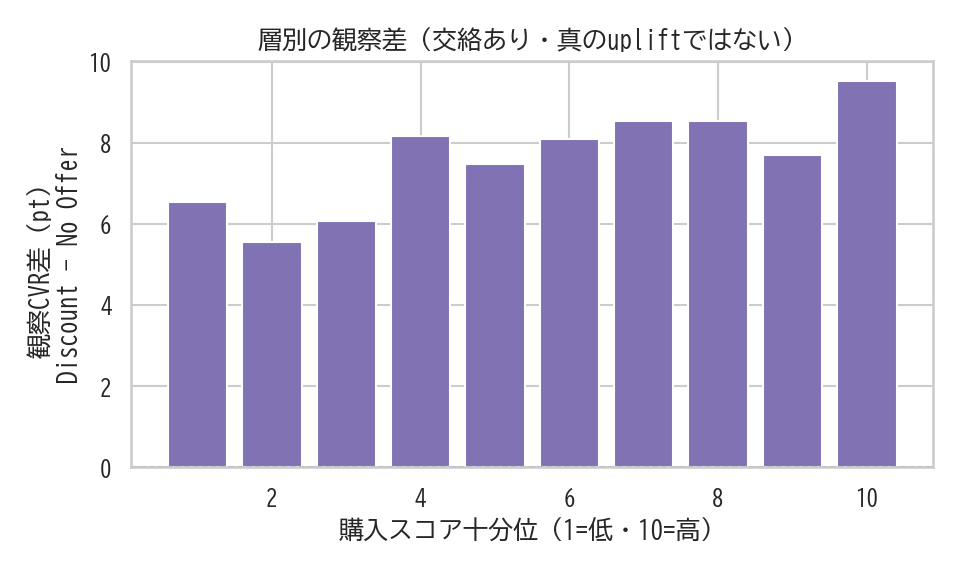
\includegraphics[width=0.88\linewidth]{../figures/improvements/uplift_crude_gap_by_score_decile.png}
  \caption{購入スコア（本スクリプトの6次元ロジスティック）十分位ごとの\textbf{観察}CVR差（Discount $-$ No Offer）。\textbf{割当は無作為ではない}ため真の増分（uplift）ではない。高スコア側で差が相対的に小さい層がありうる――\textbf{無駄割引}仮説の動機付けとして参照し、RCTで検証する。}
  \label{fig:uplift_crude_gap}
\end{figure}

\begin{table}[htbp]
  \centering
  \small
  \caption{仮定MDE（絶対差）に対する片群必要人数の目安（ベースラインCVR$=$25.00\%、上位10\%コホート。二比例・$\alpha$=0.05・正規近似）}
  \label{tab:pilot_power}
  \begin{tabular}{@{}rrrr@{}}
    \toprule
    MDE（絶対差） & 検定力 & 片群$n$（近似） & 3臂合計$n$目安 \\
    \midrule
    0.010 & 0.8 & 29821 & 89463 \\

    0.010 & 0.9 & 39921 & 119763 \\

    0.020 & 0.8 & 7550 & 22650 \\

    0.020 & 0.9 & 10107 & 30321 \\

    \bottomrule
  \end{tabular}
\end{table}

\subsection{追加で欲しいデータ（次の分析のため）}
\begin{itemize}
  \item \textbf{真の粗利・オファー別コスト・接触コスト}（会計・オペレーション連携）。
  \item \textbf{割当ルール・露出ログ}（誰がなぜそのオファーを見たかの監査証跡）。
  \item \textbf{在庫・供給・クレーム}（SUTVA違反・ネガティブ外部性の評価）。
  \item \textbf{複数期パネル}（慣習化・疲労・LTV）。
\end{itemize}

\medskip\noindent
\textbf{一般論（なぜこれらが要るか）.}
オフラインの期待利益最大化を\textbf{事業の損益}に接続するには、売上だけでなく\textbf{返品・原価・オファー毎の変動費}と\textbf{接触・配信の辺際コスト}が揃っていることが望ましい（proxy 感度分析の限界を縮める）。
\textbf{割当の決定規則}と\textbf{露出・配信ログ}（誰がいつどのクリエイティブ／オファーを見たか）は、観察データでの交絡の説明・監査に加え、RCT・\textbf{ホールドアウト}・ジオテスト等の\textbf{増分（インクリメンタル）効果}の推定において標準的な前提データである（無作為化のない記述比較だけでは処置効果に置き換えられない）。
\textbf{在庫・キャパシティ・クレーム・品切れ}は、プロモが他者の購入可能性やオペレーションに与える\textbf{外部性}を評価するのに必要で、単一期間の購入有無だけではSUTVA違反が見えにくい。
\textbf{複数期の顧客×時点データ}は、同一顧客への繰り返し接触による\textbf{疲労}や価格感応の\textbf{慣習化}、および\textbf{LTV}・チャーンとのトレードオフを分離するために不可欠である（短期CVRの改善が長期価値を損なわないかの検証）。

\medskip
% auto-generated by analytics/assumed_supplementary_analysis.py
\noindent
\textbf{数値仮定（フェルミ）.}
\texttt{history} を\textbf{円建て}の年間購買額プロキシとし、粗利率 0.32（$\sqrt{0.25\times 0.40}\approx 0.32$ のオーダー）、
キャンペーン1回の売上をその 0.083 倍（月次花弁相当・円）、
割引・BOGO の売上に対する負担をそれぞれ 25%・38% と置いた。
接触コストは Web/Multichannel/Phone で床 5.0/29.0/92.0 円に加え history の 0.6% を足す。
平均 history 242.1 円の顧客が1回購入した場合の売上目安は 20.17 円、粗利（プロモ前）は 6.46 円。
露出は期間中 Poisson($\lambda=3.2$) の合成ログ、在庫は需要CV 0.18・BOGO需要×1.35 のショック、
クレームはベース 1.5% にオファー上乗せ、パネルは累積接触に $\exp(-0.04\times\cdot)$ の疲労を仮定（詳細は付録\ref{app:assumed-data}）。


\subsection{本稿の位置づけ（ロードマップ）}
オフライン評価は\textbf{識別仮定}と\textbf{コスト・価値 proxy}に依存する。
本稿の数値は\textbf{パイロット実験}と\textbf{本番モニタリング}を前提にスケールすべきである。

\medskip\noindent
\textbf{長期・ブランド・インセンティブ疲労.}
本分析の提案は\textbf{オフライン上の期待利益 proxy の最大化}にフォーカスする。
\textbf{割引の乱発によるブランド毀損・価格感応度の習慣化・長期LTVの低下}は、本データに直接は含まれないため、別途パネルデータやブランド調査で監視することが望ましい。

\medskip\noindent
\textbf{公平性・地域属性.}
\texttt{zip\_code} 等の地域カテゴリは差別的配信やセンシティブ属性の proxy になりうる。
\textbf{地域属性のみを理由とした不利益な差別的取り扱いにならないよう、ガバナンス上のレビューと利用目的の限定}を前提とする（本文の倫理表と併せて運用する）。

\subsection{最終課題への適合性と改善余地（自己査読）}
\noindent
\textbf{課題文との対応.}
「購入確度の高いユーザーの傾向」については、EDA・予測モデル・セグメント記述および表\ref{tab:pilot_cohort}・表\ref{tab:pilot_profile_binary}で層別の記述を示している。
「その層にプロモを打つ」については、スコア上位の\textbf{記述CVR}と\textbf{ターゲティング方針}に加え、コストを入れた\textbf{期待利益 proxy}と\textbf{制約付き割当}まで踏み込んでいる。
「新施策」については、パイロットRCT・運用ゲート・監視・付録の仮定ベース感度が整理されている。
よって\textbf{要件の骨格は満たす}。

\medskip\noindent
\textbf{世界標準の実務・研究から見た強み.}
問題設定が\textbf{増分性（uplift）とオフライン方針評価のギャップ}を明示している点、多値介入に\textbf{DR＋OOF}を接続している点、\textbf{倫理・モニタリング・実験計画}まで一気通貫している点は、産業界の「MLOps＋因果」の良い型に近い。

\medskip\noindent
\textbf{残る改善余地.}
\begin{itemize}
  \item \textbf{簡潔さ}：診断図の一部を付録へ移し、本編を「結論・識別・主要KPI」に絞ると、授業レポートとしてさらに読みやすい。
  \item \textbf{本番データ接続}：真の粗利・接触コスト・割当ログが揃えば、オフライン政策とP\&Lのギャップをさらに縮小できる。
\end{itemize}

\begin{thebibliography}{99}
\bibitem{Rosenbaum1983}
Paul~R. Rosenbaum and Donald~B. Rubin.
\newblock The central role of the propensity score in observational studies for causal effects.
\newblock \textit{Biometrika}, 70(1):41--55, 1983.

\bibitem{BangRobins2005}
Heejung Bang and James~M. Robins.
\newblock Doubly robust estimation in missing data and causal inference models.
\newblock \textit{Biometrics}, 61(4):962--973, 2005.

\bibitem{Dudik2011}
Miroslav Dud\'ik, John Langford, and Lihong Li.
\newblock Doubly robust policy evaluation and learning.
\newblock In \textit{Proceedings of ICML}, 2011.

\bibitem{ImbensRubin2015}
Guido~W. Imbens and Donald~B. Rubin.
\newblock \textit{Causal Inference for Statistics, Social, and Biomedical Sciences}.
\newblock Cambridge University Press, 2015.

\bibitem{Kohavi2020}
Ron Kohavi, Diane Tang, and Ya Xu.
\newblock \textit{Trustworthy Online Controlled Experiments: A Practical Guide to A/B Testing}.
\newblock Cambridge University Press, 2020.

\bibitem{Gordon2019}
Brett~R. Gordon, Florian Zettelmeyer, Neha Bhargava, and Dan Chapsky.
\newblock A comparison of approaches to advertising measurement: Evidence from big field experiments at Facebook.
\newblock \textit{Marketing Science}, 38(2):193--225, 2019.
\end{thebibliography}

\appendix

\section*{付録の位置づけ}
\noindent
付録は\textbf{再現手順}、\textbf{中間成果物の所在}、および\textbf{仮定ベースの補完分析}（\texttt{exercise.csv} に無い要素のデモ）をまとめる。
本編の結論を変える主張は行わず、感度・監査・実装のための材料として利用する。

\section{限界と免責}
\begin{itemize}
  \item \textbf{観察データ}: 未観測交絡、SUTVA 違反、慣習化（\texttt{risk\_register.json} 参照）。
  \item \textbf{ブートストラップ}: 部分標本再学習であり、厳密な頑健区間の代替ではない。
  \item \textbf{法的助言}: 本稿は法的・コンプライアンス上の助言を構成しない。
\end{itemize}

\section{付録：データスニペットの再現方法}
表 \ref{tab:data_examples} とデータ概要の箇条書きは、リポジトリ直下の \texttt{exercise.csv} から
\texttt{python -S scripts/build\_latex\_data\_snippets.py}（または通常の \texttt{python}）で
\texttt{latex/data\_overview\_snippet.tex} と \texttt{latex/data\_sample\_table.tex} を再生成できる。

\section{付録：コスト感度表の再現方法}
表 \ref{tab:cost_sensitivity_modes} は \texttt{artifacts/profit\_long.csv} から
\texttt{python -S scripts/build\_cost\_sensitivity\_from\_profit\_long.py} で再生成できる。

\section{付録：本文で詳述しきれなかった出力物}
詳細な数表・中間成果物は \texttt{artifacts/} に集約する（例：\texttt{chi2\_tests\_with\_fdr.csv}、\texttt{promo\_targets*.csv}、\texttt{policy\_eval\_compare.csv}、\texttt{segment\_treatment\_cvr\_exploratory.csv}）。
Markdown 版の長い考察は \texttt{final\_report.md} を参照。

\section{付録：仮定データによる補完分析（図表・サンプル・コード）}
\label{app:assumed-data}

\noindent
\texttt{exercise.csv} には粗利・真の接触コスト・露出ログ・在庫・複数期パネルが含まれない。
本節では、\textbf{フェルミ推定でオーダーを揃えた仮定}（\texttt{artifacts/assumed\_data\_fermi.json}）のもとで
会計風の利益分解・合成露出・在庫モンテカルロ・疲労付き合成LTVを\textbf{デモ}として付す。
解釈はすべて\textbf{演習上の感度・監査イメージ}であり、事業数値の断定や因果効果の主張ではない。

% auto-generated by analytics/assumed_supplementary_analysis.py
\paragraph{接触コスト（円）のフェルミ推定.}
\noindent
\textbf{Web.} 一斉メール等の限界費用を 0.5--2.0 円/通、ESP・創出の按分を 2--10 円/接触の帯とし、オーダーを足し合わせて床を \textbf{5}~円とした（限界費用帯と按分帯の幾何平均を合成し、最低 \textbf{5}~円でキャップ）。

\noindent
\textbf{Multichannel.} Web 床に SMS/プッシュ等の追加分 18--30 円の中央 （24 円）を加え、床 \textbf{29}~円。

\noindent
\textbf{Phone.} 架電オペの時給負担（人件費・諸掛）を 2000--2800 円/時、実効接触を 20--32 件/時と置き、中央 2400/26.0 $\approx$ 92.3 円/接触 $\rightarrow$ 床 \textbf{92}~円。

\noindent
\textbf{\texttt{history} 比例項.} 年間購買額プロキシに対する変動オペ・差し替え負担を 0.4%--0.8% とし、\textbf{0.6%} を採用。


% auto-generated — figures in ../figures/appendix/（subcaption で横並び）
\begin{figure}[!htbp]
  \centering
  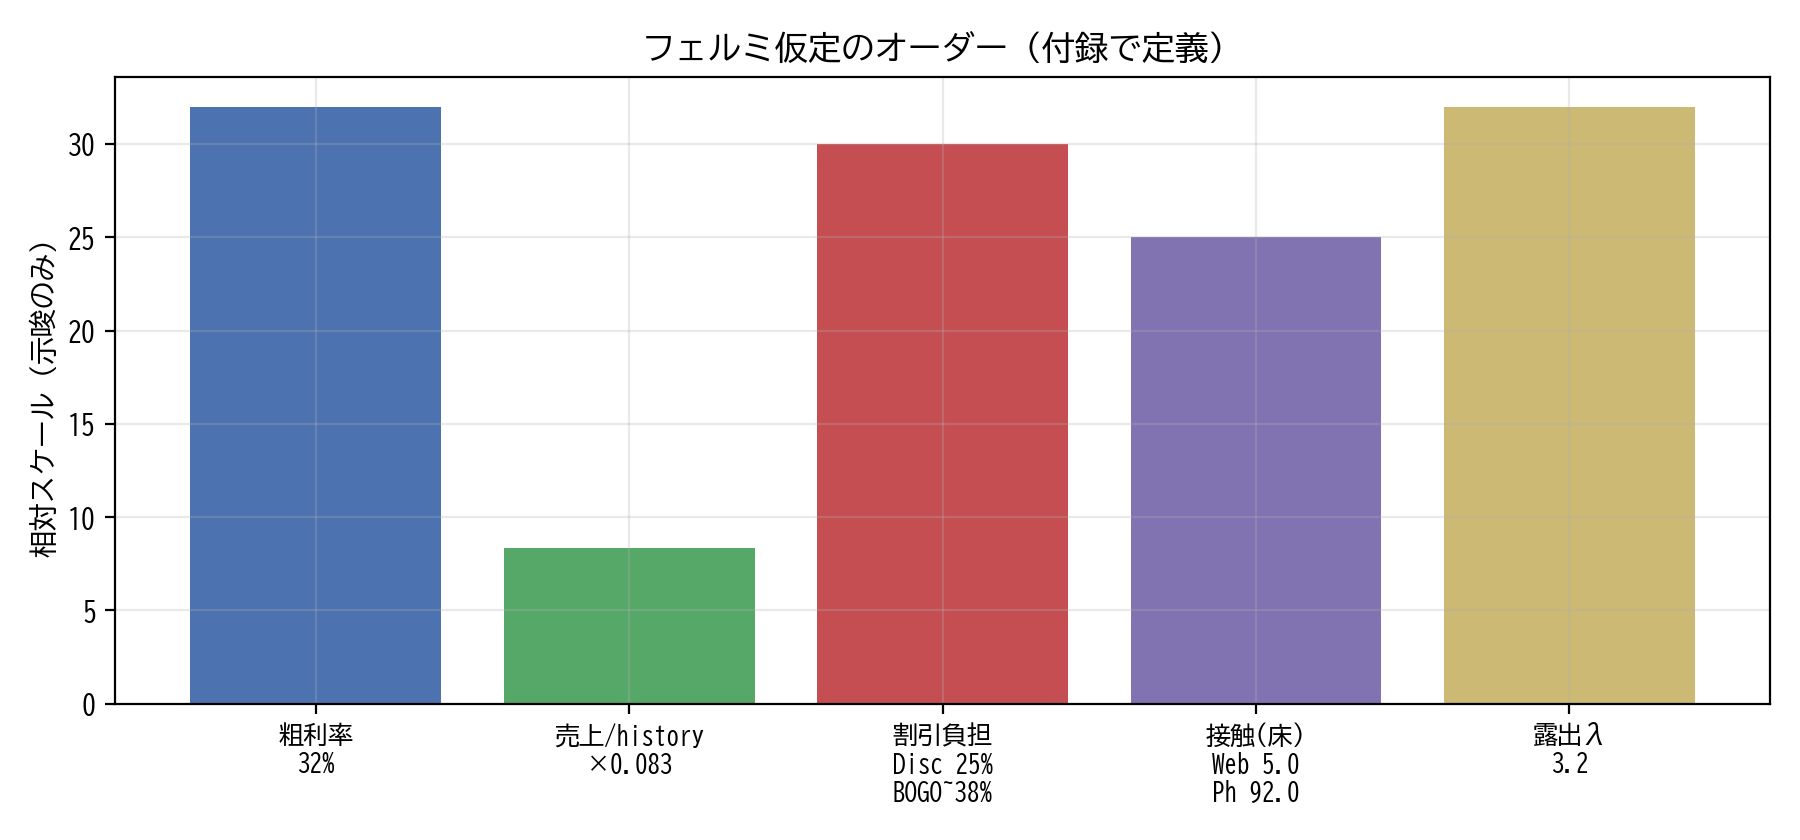
\includegraphics[width=0.88\linewidth]{../figures/appendix/fig_fermi_schematic.png}
  \caption{フェルミ仮定のオーダー（粗利・売上スケール・オファー負担・接触・露出）。}
  \label{fig:app-fermi-schematic}
\end{figure}

\begin{figure}[!htbp]
  \centering
  \begin{subfigure}[t]{0.49\linewidth}
    \centering
    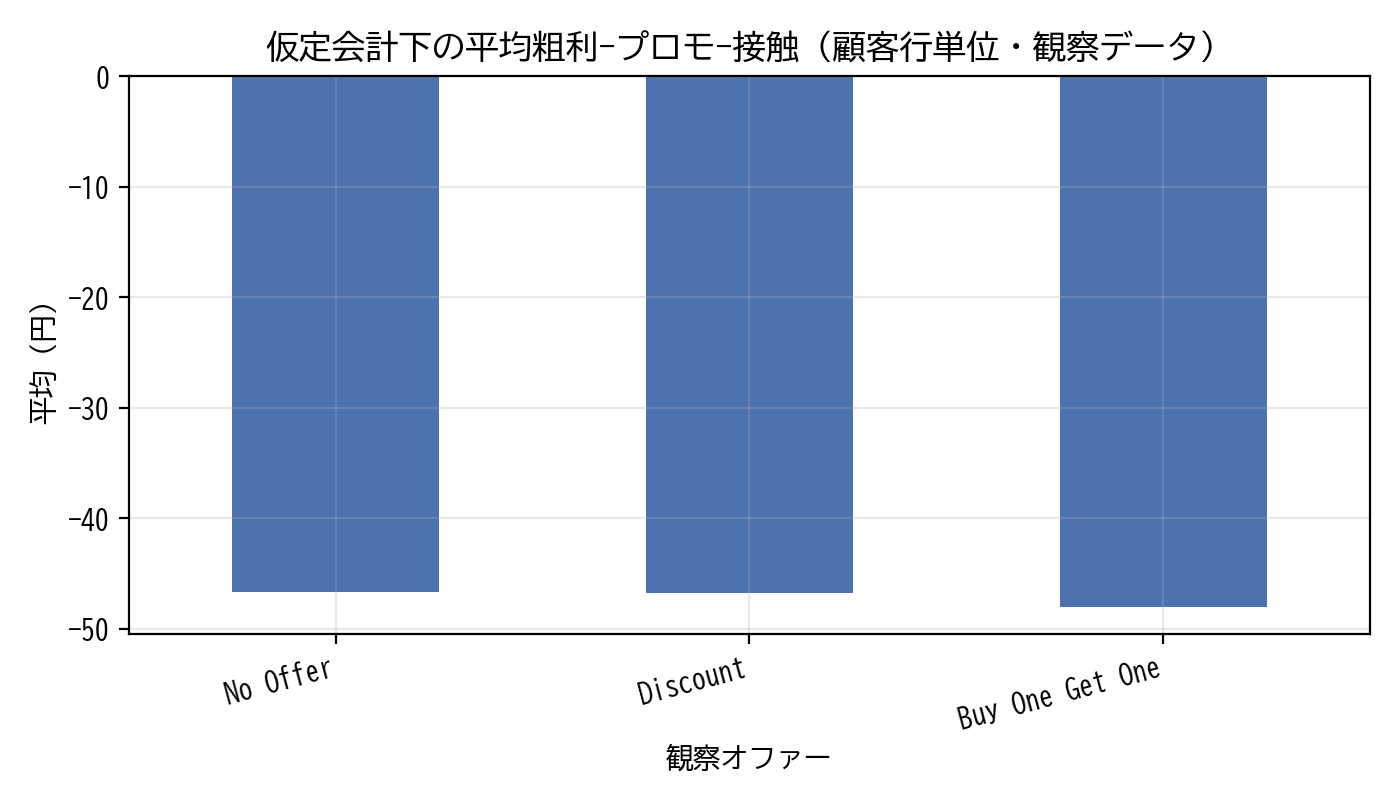
\includegraphics[width=\linewidth]{../figures/appendix/fig_profit_by_observed_offer.png}
    \caption{観察オファー別の平均利益（粗利−プロモ−接触）。因果効果ではない。}
    \label{fig:app-profit-offer}
  \end{subfigure}\hfill
  \begin{subfigure}[t]{0.49\linewidth}
    \centering
    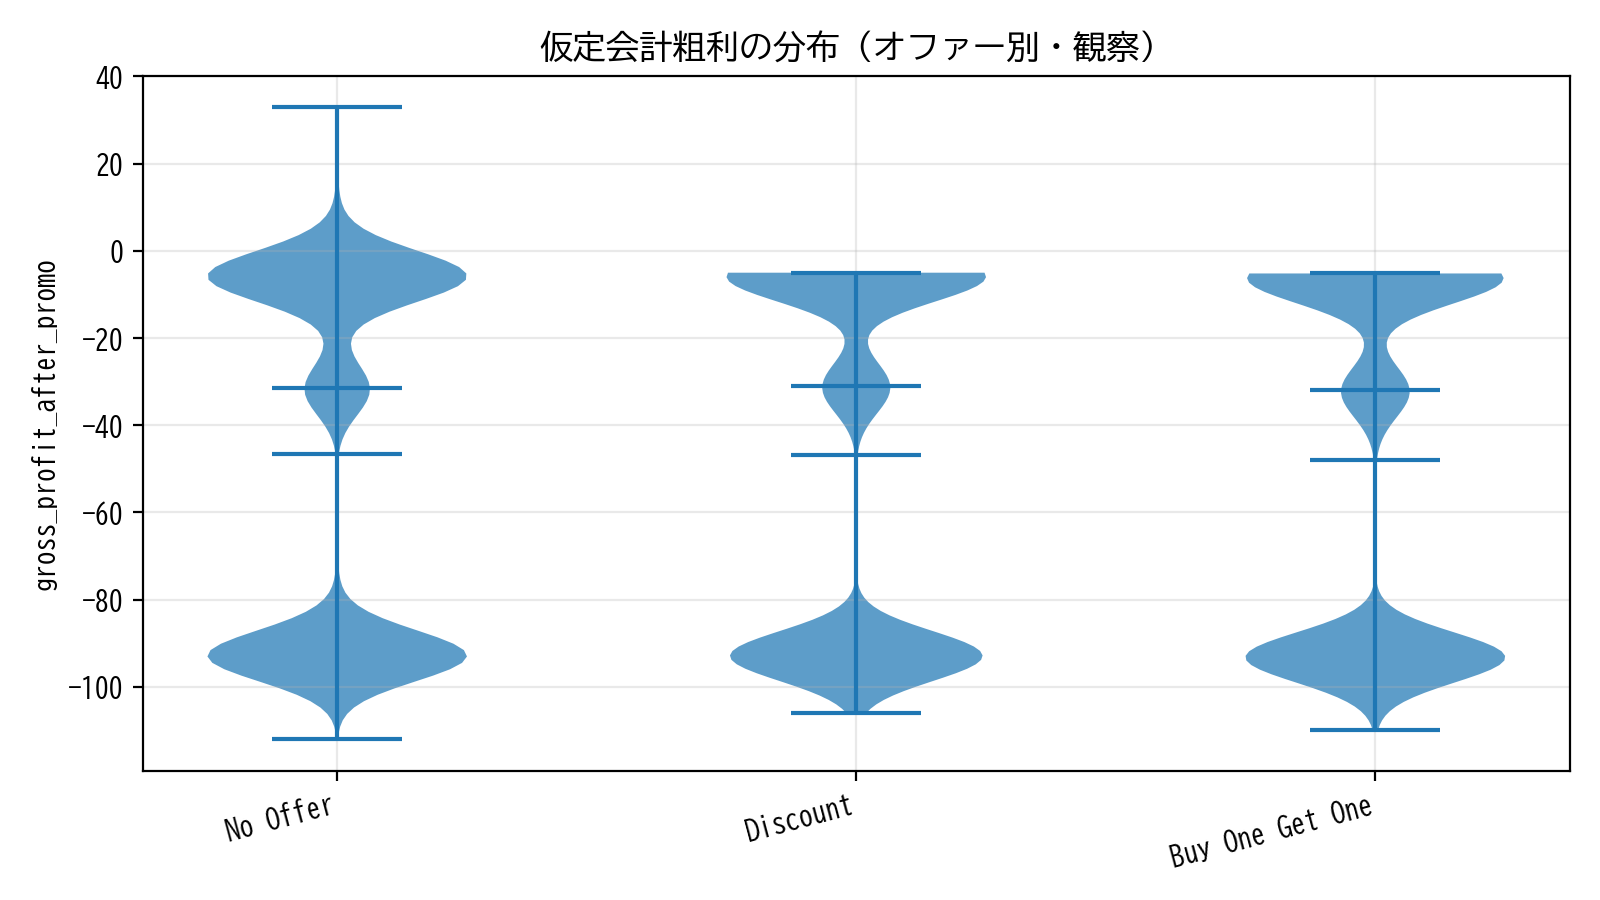
\includegraphics[width=\linewidth]{../figures/appendix/fig_gp_violin_by_offer.png}
    \caption{同・仮定会計での利益分布（バイオリン）。}
    \label{fig:app-gp-violin}
  \end{subfigure}
  \caption{仮定会計におけるオファー別の水準と分布}
\end{figure}

\begin{figure}[!htbp]
  \centering
  \begin{subfigure}[t]{0.49\linewidth}
    \centering
    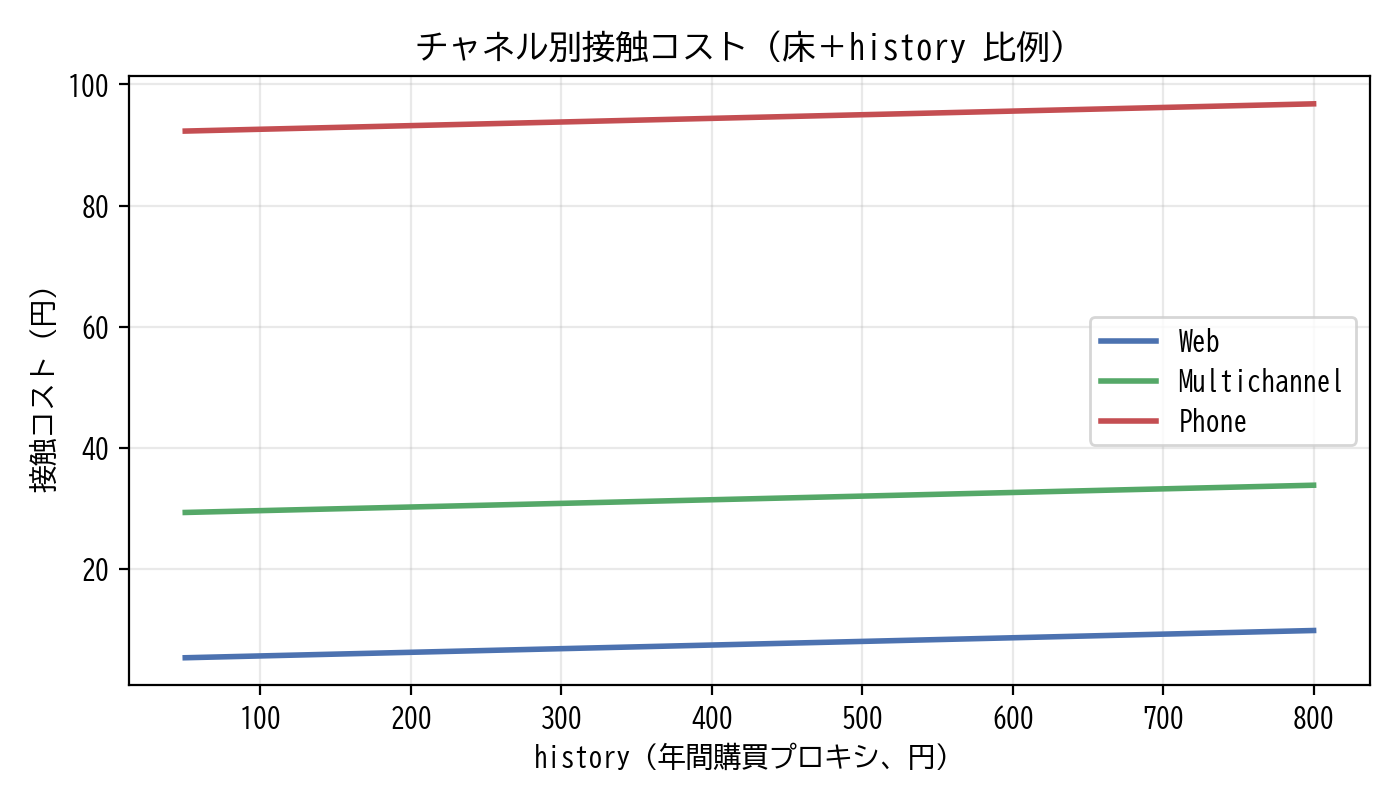
\includegraphics[width=\linewidth]{../figures/appendix/fig_contact_cost_by_channel.png}
    \caption{チャネル別の接触コスト曲線（床＋history比例）。}
    \label{fig:app-contact}
  \end{subfigure}\hfill
  \begin{subfigure}[t]{0.49\linewidth}
    \centering
    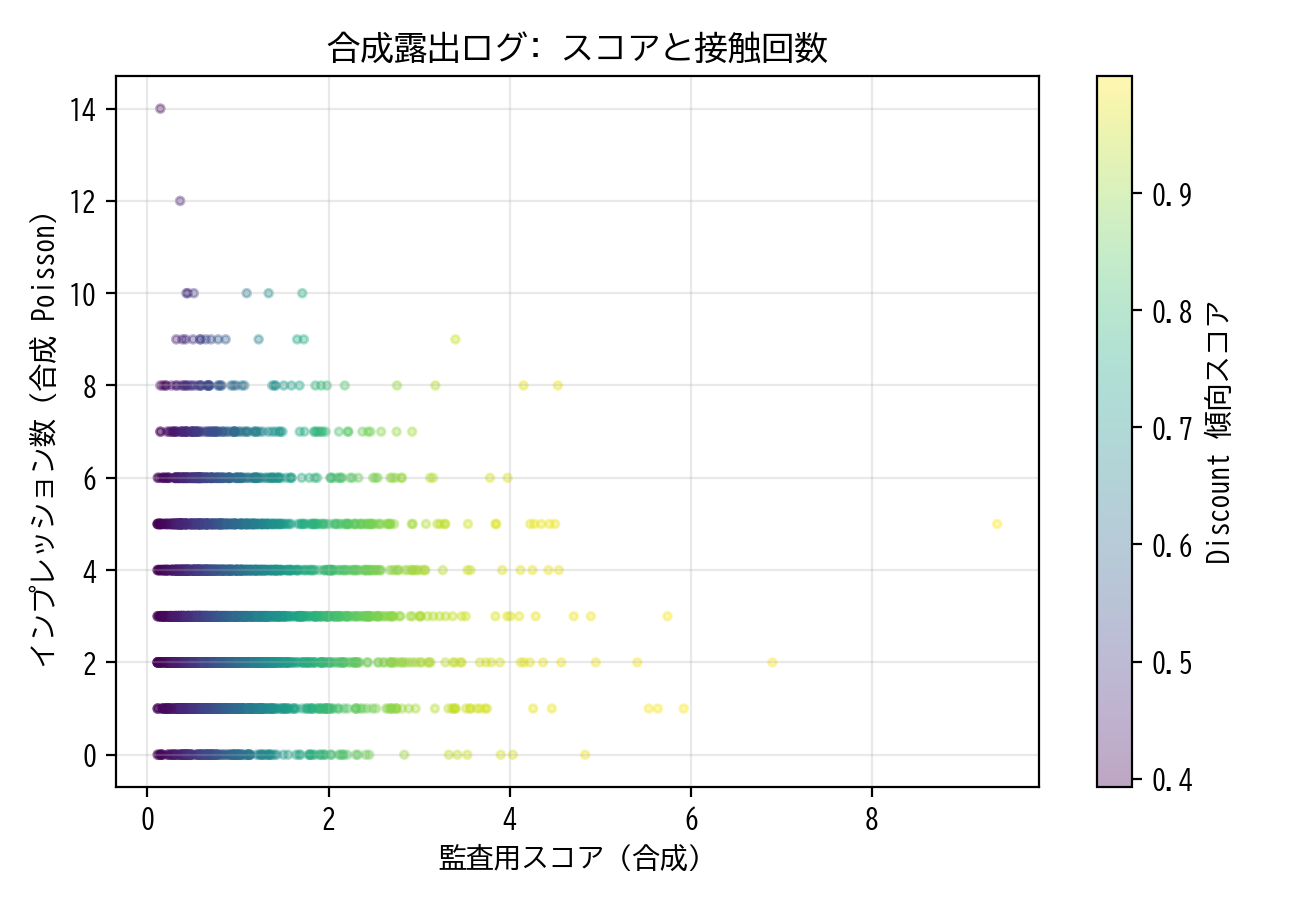
\includegraphics[width=\linewidth]{../figures/appendix/fig_exposure_scatter_audit.png}
    \caption{合成露出ログ：監査スコアとインプレッション数。}
    \label{fig:app-exposure}
  \end{subfigure}
  \caption{接触コストと合成露出}
\end{figure}

\begin{figure}[!htbp]
  \centering
  \begin{subfigure}[t]{0.49\linewidth}
    \centering
    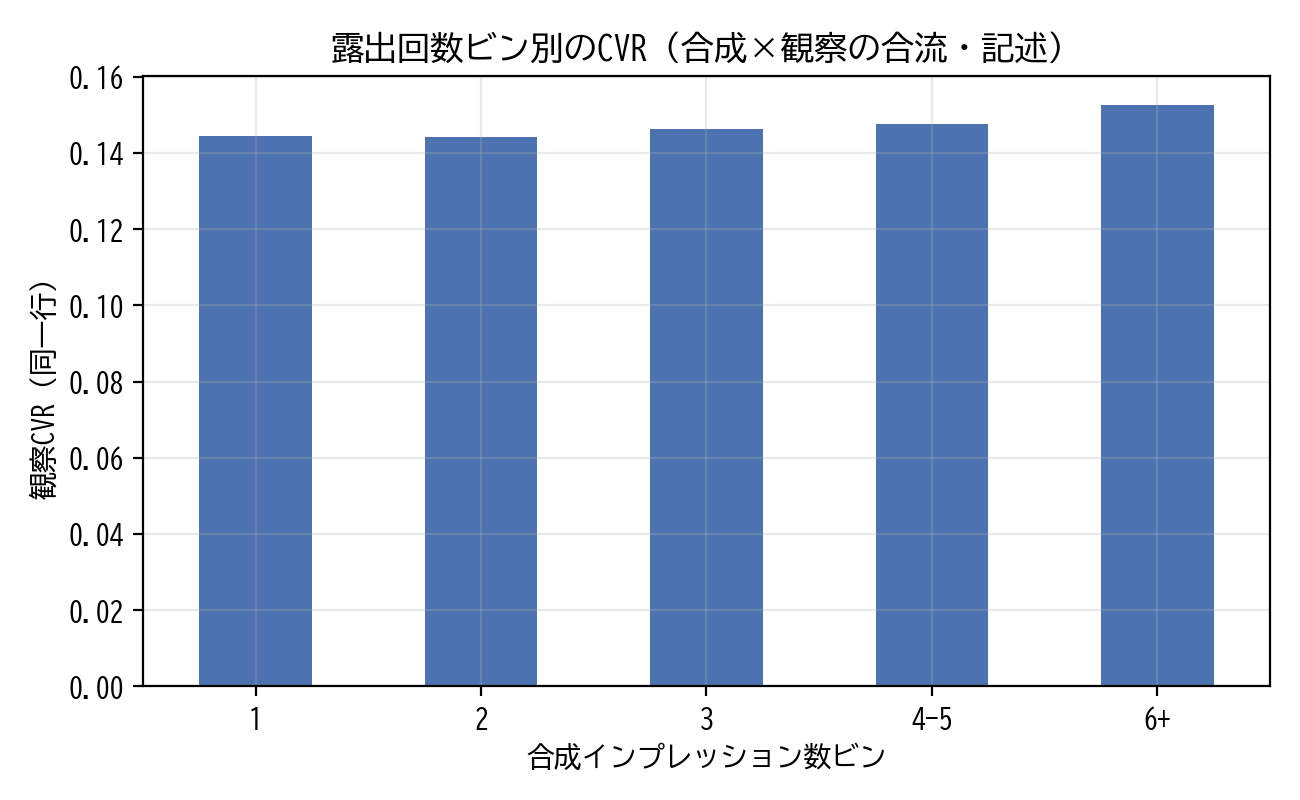
\includegraphics[width=\linewidth]{../figures/appendix/fig_cvr_by_impression_bin.png}
    \caption{インプレッション数ビン別の観察CVR（記述）。}
    \label{fig:app-cvr-imp}
  \end{subfigure}\hfill
  \begin{subfigure}[t]{0.49\linewidth}
    \centering
    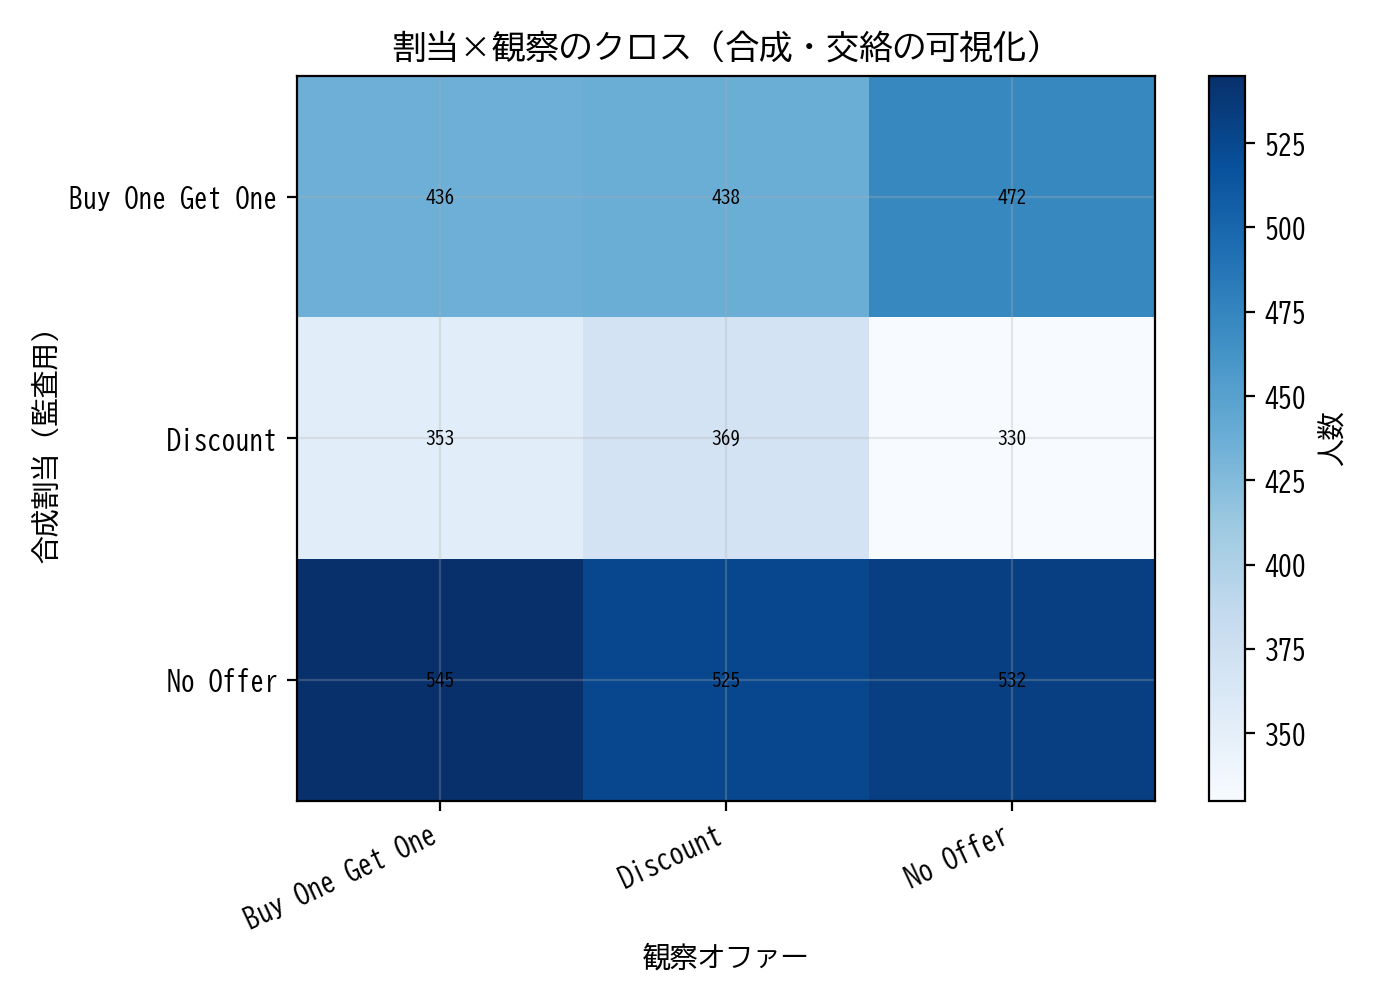
\includegraphics[width=\linewidth]{../figures/appendix/fig_assignment_cross_heatmap.png}
    \caption{合成割当と観察オファーのクロス。}
    \label{fig:app-assign-heat}
  \end{subfigure}
  \caption{合成ログに基づく記述（左：CVRビン、右：割当クロス）}
\end{figure}

\begin{figure}[!htbp]
  \centering
  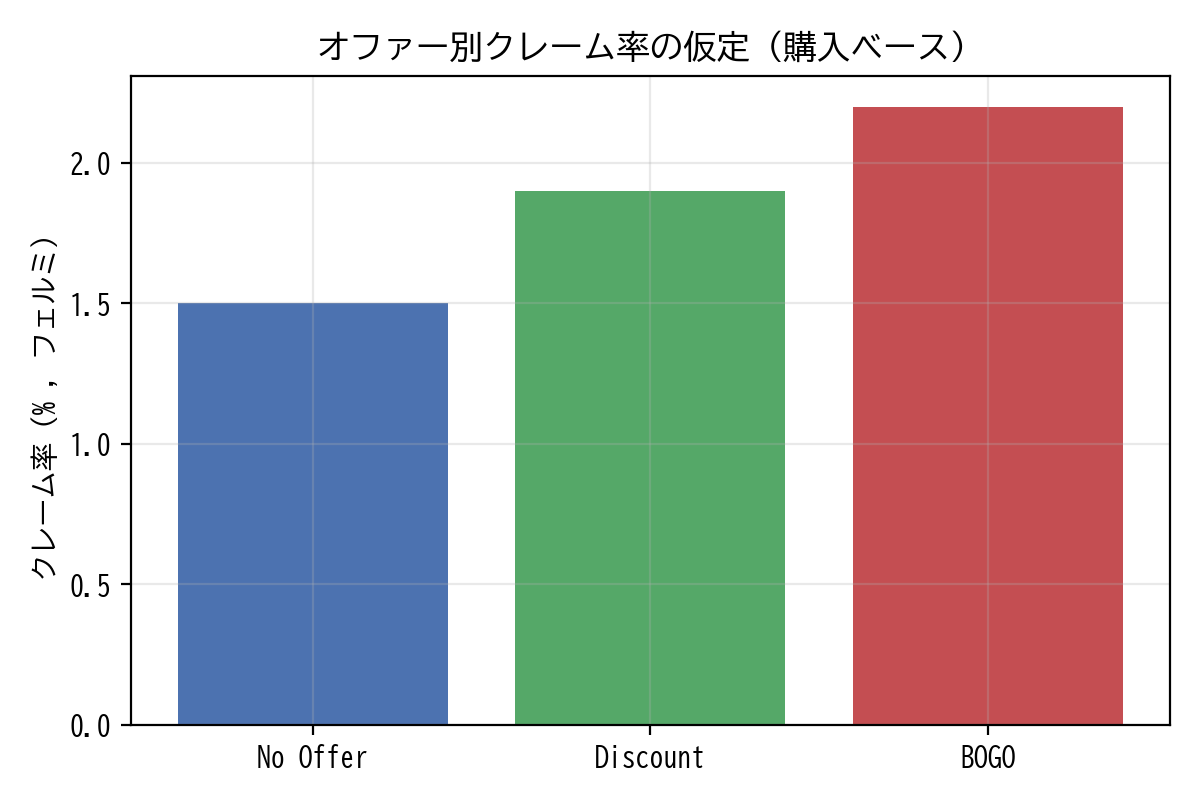
\includegraphics[width=0.92\linewidth]{../figures/appendix/fig_claims_rate_by_offer.png}
  \caption{オファー別クレーム率のフェルミ仮定。}
  \label{fig:app-claims}
\end{figure}

\begin{figure}[!htbp]
  \centering
  \begin{subfigure}[t]{0.49\linewidth}
    \centering
    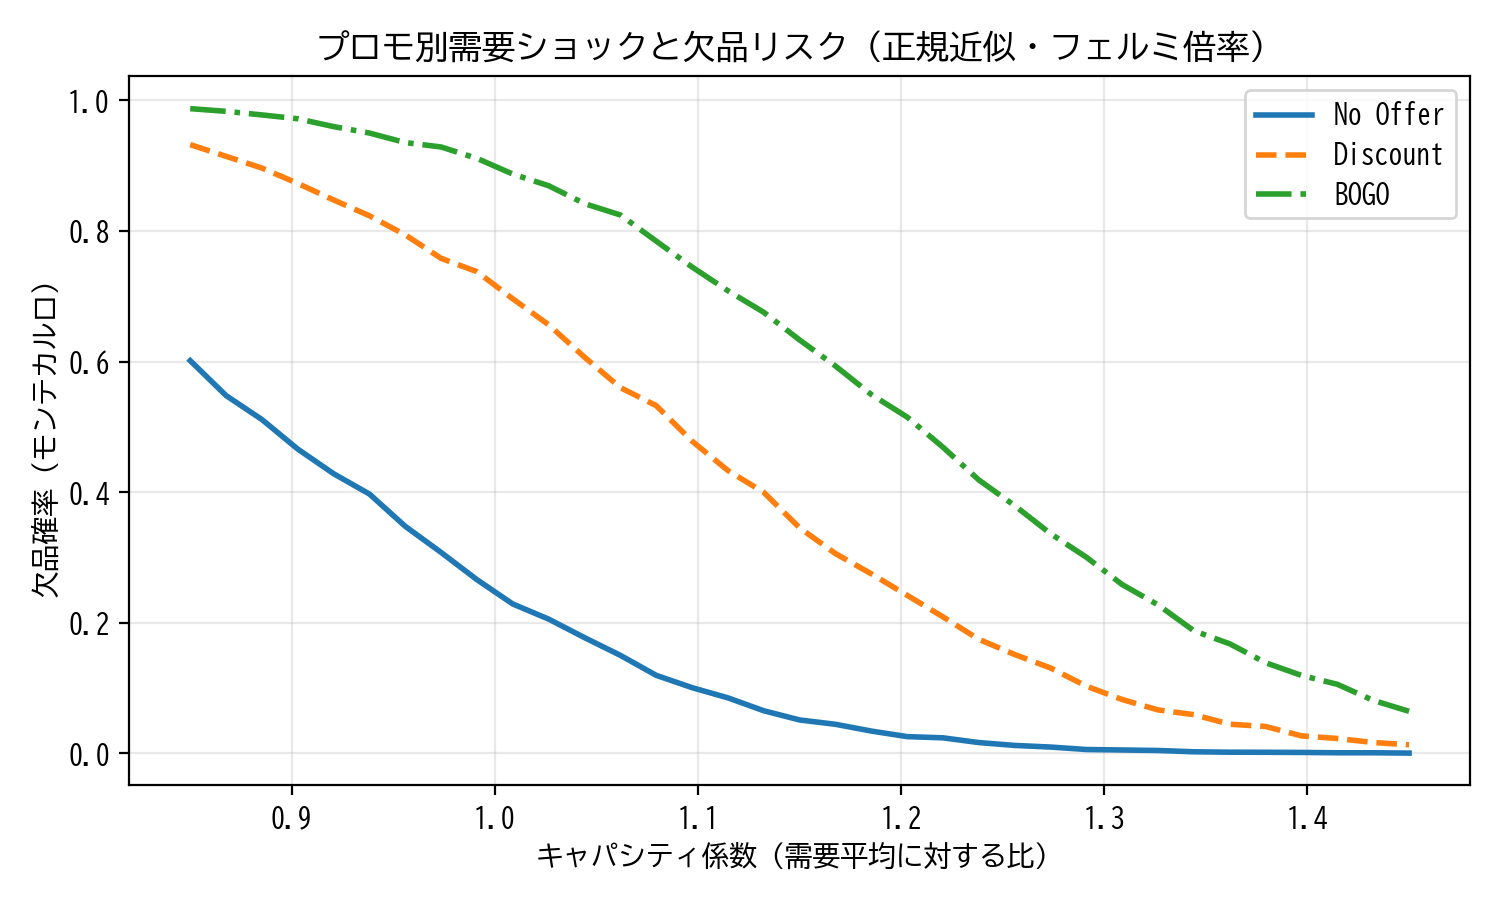
\includegraphics[width=\linewidth]{../figures/appendix/fig_inventory_stockout.png}
    \caption{需要ショックに対する欠品確率（モンテカルロ）。}
    \label{fig:app-inventory}
  \end{subfigure}\hfill
  \begin{subfigure}[t]{0.49\linewidth}
    \centering
    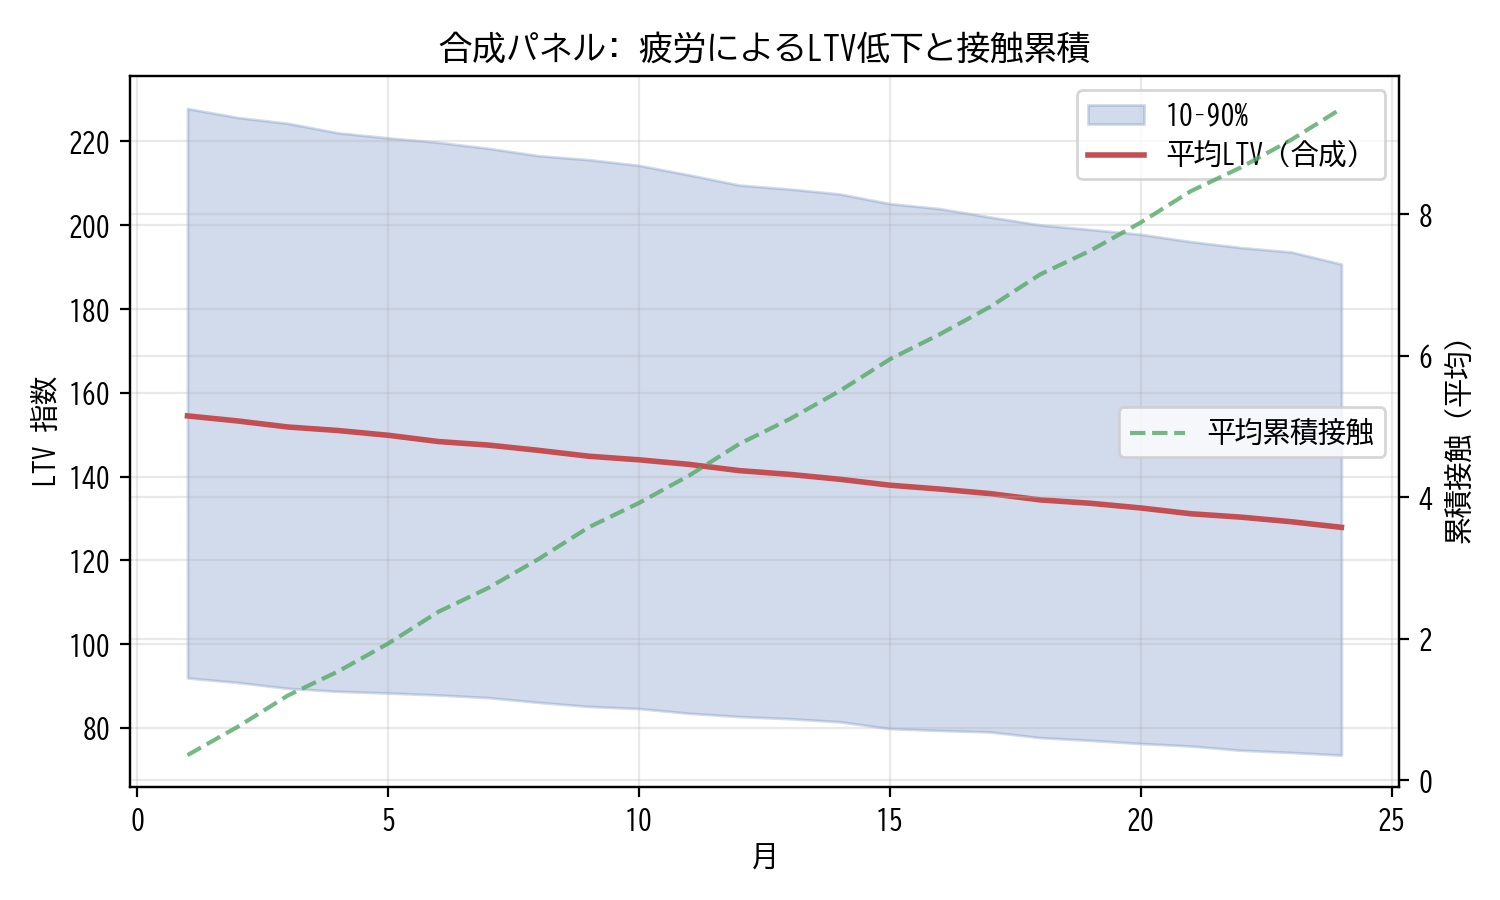
\includegraphics[width=\linewidth]{../figures/appendix/fig_panel_ltv_fatigue.png}
    \caption{合成パネル：LTVと累積接触（疲労）。}
    \label{fig:app-panel}
  \end{subfigure}
  \caption{在庫リスクと長期パネル（合成）}
\end{figure}

\begin{figure}[!htbp]
  \centering
  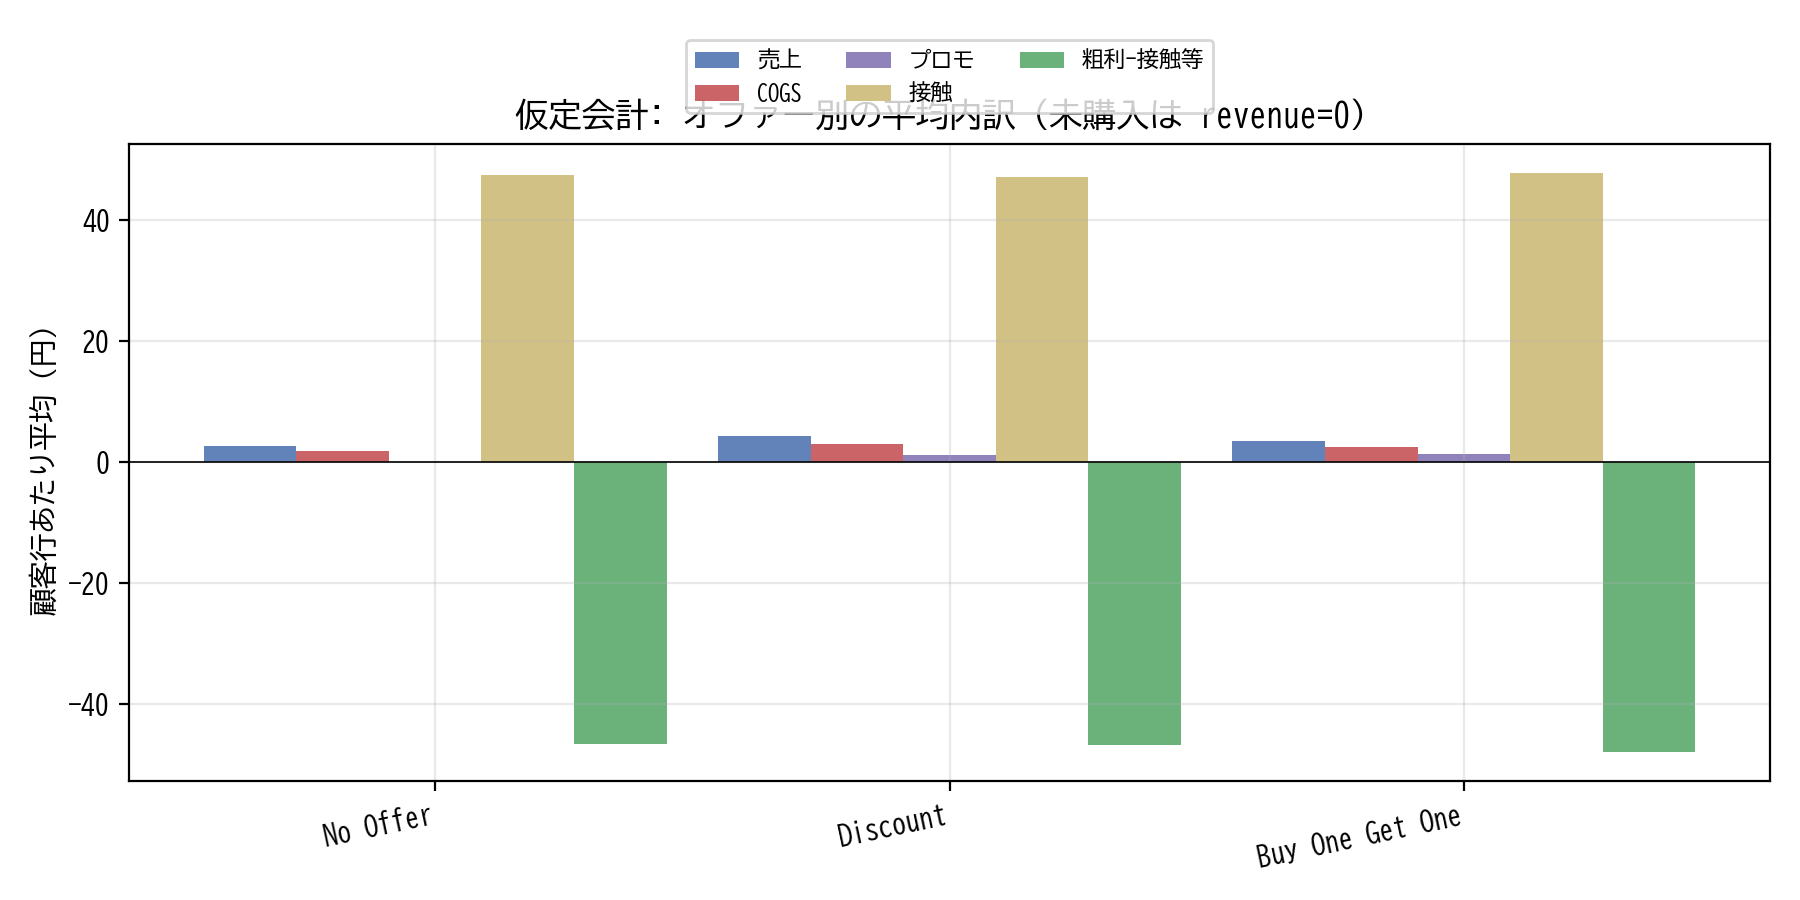
\includegraphics[width=0.92\linewidth]{../figures/appendix/fig_profit_components_grouped.png}
  \caption{仮定会計におけるオファー別の平均内訳（売上・COGS・プロモ・接触・粗利）。凡例は図内の棒グラフの下に配置。}
  \label{fig:app-profit-grouped}
\end{figure}


\subsection{仮定パラメータ（JSON）}
\noindent
パラメータの機械可読な一覧は \texttt{artifacts/assumed\_data\_fermi.json}（\texttt{python -m analytics.assumed\_supplementary\_analysis} で再生成）。本文の数値は円建て \texttt{history} との整合を前提とする。

\subsection{データセット抜粋（演習用 \texttt{exercise.csv}）}
\noindent
全件はリポジトリ直下の \texttt{exercise.csv}。
先頭500行は \texttt{artifacts/appendix\_exercise\_sample.csv}。以下は\textbf{先頭12行のみ}（全列）。

\lstinputlisting[
  caption={\texttt{appendix\_exercise\_sample.csv} 先頭12行},
  label={lst:exercise-sample},
  firstline=1,
  lastline=12,
]{../artifacts/appendix_exercise_sample.csv}

\subsection{合成露出ログ抜粋}
\lstinputlisting[
  caption={\texttt{synthetic\_exposure\_log\_sample.csv} 先頭10行},
  label={lst:exposure-sample},
  firstline=1,
  lastline=10,
]{../artifacts/synthetic_exposure_log_sample.csv}

\subsection{分析に用いた Python コード}
\noindent
\textbf{全文}は \texttt{analytics/assumed\_supplementary\_analysis.py}。再現は \texttt{python -m analytics.assumed\_supplementary\_analysis}。
以下は\textbf{モジュール先頭と \texttt{FermiAssumptions} 定義部の抜粋}（円建て \texttt{history} のコメント含む）。

\lstinputlisting[
  language=Python,
  caption={\texttt{assumed\_supplementary\_analysis.py} 抜粋（先頭58行・\texttt{FermiAssumptions} 途中まで）},
  label={lst:assumed-py},
  firstline=1,
  lastline=58,
]{../analytics/assumed_supplementary_analysis.py}

\end{document}
